\documentclass[twoside]{book}

% Packages required by doxygen
\usepackage{fixltx2e}
\usepackage{calc}
\usepackage{doxygen}
\usepackage[export]{adjustbox} % also loads graphicx
\usepackage{graphicx}
\usepackage[utf8]{inputenc}
\usepackage{makeidx}
\usepackage{multicol}
\usepackage{multirow}
\PassOptionsToPackage{warn}{textcomp}
\usepackage{textcomp}
\usepackage[nointegrals]{wasysym}
\usepackage[table]{xcolor}

% Font selection
\usepackage[T1]{fontenc}
\usepackage[scaled=.90]{helvet}
\usepackage{courier}
\usepackage{amssymb}
\usepackage{sectsty}
\renewcommand{\familydefault}{\sfdefault}
\allsectionsfont{%
  \fontseries{bc}\selectfont%
  \color{darkgray}%
}
\renewcommand{\DoxyLabelFont}{%
  \fontseries{bc}\selectfont%
  \color{darkgray}%
}
\newcommand{\+}{\discretionary{\mbox{\scriptsize$\hookleftarrow$}}{}{}}

% Page & text layout
\usepackage{geometry}
\geometry{%
  a4paper,%
  top=2.5cm,%
  bottom=2.5cm,%
  left=2.5cm,%
  right=2.5cm%
}
\tolerance=750
\hfuzz=15pt
\hbadness=750
\setlength{\emergencystretch}{15pt}
\setlength{\parindent}{0cm}
\setlength{\parskip}{3ex plus 2ex minus 2ex}
\makeatletter
\renewcommand{\paragraph}{%
  \@startsection{paragraph}{4}{0ex}{-1.0ex}{1.0ex}{%
    \normalfont\normalsize\bfseries\SS@parafont%
  }%
}
\renewcommand{\subparagraph}{%
  \@startsection{subparagraph}{5}{0ex}{-1.0ex}{1.0ex}{%
    \normalfont\normalsize\bfseries\SS@subparafont%
  }%
}
\makeatother

% Headers & footers
\usepackage{fancyhdr}
\pagestyle{fancyplain}
\fancyhead[LE]{\fancyplain{}{\bfseries\thepage}}
\fancyhead[CE]{\fancyplain{}{}}
\fancyhead[RE]{\fancyplain{}{\bfseries\leftmark}}
\fancyhead[LO]{\fancyplain{}{\bfseries\rightmark}}
\fancyhead[CO]{\fancyplain{}{}}
\fancyhead[RO]{\fancyplain{}{\bfseries\thepage}}
\fancyfoot[LE]{\fancyplain{}{}}
\fancyfoot[CE]{\fancyplain{}{}}
\fancyfoot[RE]{\fancyplain{}{\bfseries\scriptsize Generated by Doxygen }}
\fancyfoot[LO]{\fancyplain{}{\bfseries\scriptsize Generated by Doxygen }}
\fancyfoot[CO]{\fancyplain{}{}}
\fancyfoot[RO]{\fancyplain{}{}}
\renewcommand{\footrulewidth}{0.4pt}
\renewcommand{\chaptermark}[1]{%
  \markboth{#1}{}%
}
\renewcommand{\sectionmark}[1]{%
  \markright{\thesection\ #1}%
}

% Indices & bibliography
\usepackage{natbib}
\usepackage[titles]{tocloft}
\setcounter{tocdepth}{3}
\setcounter{secnumdepth}{5}
\makeindex

% Hyperlinks (required, but should be loaded last)
\usepackage{ifpdf}
\ifpdf
  \usepackage[pdftex,pagebackref=true]{hyperref}
\else
  \usepackage[ps2pdf,pagebackref=true]{hyperref}
\fi
\hypersetup{%
  colorlinks=true,%
  linkcolor=blue,%
  citecolor=blue,%
  unicode%
}

% Custom commands
\newcommand{\clearemptydoublepage}{%
  \newpage{\pagestyle{empty}\cleardoublepage}%
}

\usepackage{caption}
\captionsetup{labelsep=space,justification=centering,font={bf},singlelinecheck=off,skip=4pt,position=top}

%===== C O N T E N T S =====

\begin{document}

% Titlepage & ToC
\hypersetup{pageanchor=false,
             bookmarksnumbered=true,
             pdfencoding=unicode
            }
\pagenumbering{roman}
\begin{titlepage}
\vspace*{7cm}
\begin{center}%
{\Large Wave\+Simulator }\\
\vspace*{1cm}
{\large Generated by Doxygen 1.8.11}\\
\end{center}
\end{titlepage}
\clearemptydoublepage
\tableofcontents
\clearemptydoublepage
\pagenumbering{arabic}
\hypersetup{pageanchor=true}

%--- Begin generated contents ---
\chapter{Wavepropagation-\/\+Simulation on Android-\/\+Systems}
\label{index}\hypertarget{index}{}\begin{DoxyAuthor}{Author}
Gregor, Martin and Sven
\end{DoxyAuthor}
\hypertarget{index_i}{}\section{Intro}\label{index_i}
This project uses the open-\/source S\+W\+E-\/implementation, to allow the user to set up any desired Tsunami scenario, placeable objects in an given domain of calmed water.\hypertarget{index_f}{}\section{Functions}\label{index_f}
\hypertarget{index_sf}{}\subsection{Creating Waves}\label{index_sf}
The user can create waves of variable height by tapping the domain. The height can be adjusted via the Wave-\/\+Hight-\/\+Slider below the water domain. \hypertarget{index_sf1}{}\subsection{Creating Obstacles}\label{index_sf1}
The user can create equally high obstacles by selecting the draw mode(brush Symbol in the top right corner). While pressing once in this mode will result in a circular obstacle, moving around allows for the creation of any desired shape. \hypertarget{index_Removing}{}\subsection{Obstacles}\label{index_Removing}
This can be done in the same fashion as the creation, as long as the Erase\+\_\+\+Mode is chosen(minus-\/symbol on top of the domain). Tapping once will activate the Erase\+\_\+\+Mode. Tapping again will change the mode back to normal. \hypertarget{index_Boundaries}{}\subsection{Boundaries}\label{index_Boundaries}
The domain-\/boundaries can be chosen to be reflective or open. This is done by tapping the \char`\"{}\+Reflective Boundaries\char`\"{} switch located below the domain. \hypertarget{index_Resetting}{}\subsection{Resetting}\label{index_Resetting}
The user can choose to reset only the waves or the whole domain. This is done by tapping the options button in the top right corner of the screen and then choosing the wanted option. 
\chapter{Deprecated List}
\label{deprecated}
\hypertarget{deprecated}{}

\begin{DoxyRefList}
\item[\label{deprecated__deprecated000001}%
\hypertarget{deprecated__deprecated000001}{}%
Member \hyperlink{help_8hh_aa10dc278c6ac60f9cd49955cbe16fbcb}{generate\+File\+Name} (std\+::string base\+Name, int time\+Step)]
\item[\label{deprecated__deprecated000003}%
\hypertarget{deprecated__deprecated000003}{}%
Member \hyperlink{help_8hh_ab05bce4e4d30d0b9fb85f81668f98f79}{generate\+File\+Name} (std\+::string base\+Name, int time\+Step, int block\+\_\+X, int block\+\_\+Y, std\+::string i\+\_\+file\+Extension=\char`\"{}.\+vts\char`\"{})]
\item[\label{deprecated__deprecated000002}%
\hypertarget{deprecated__deprecated000002}{}%
Member \hyperlink{help_8hh_a206f33ce37fa47f8635d02a1cfc9881f}{generate\+File\+Name} (std\+::string i\+\_\+base\+Name, int i\+\_\+block\+PositionX, int i\+\_\+block\+PositionY, std\+::string i\+\_\+file\+Extension=\char`\"{}.\+nc\char`\"{})]
\end{DoxyRefList}
\chapter{Namespace Index}
\section{Namespace List}
Here is a list of all namespaces with brief descriptions\+:\begin{DoxyCompactList}
\item\contentsline{section}{\hyperlink{namespaceInterface}{Interface} \\*The \hyperlink{namespaceInterface}{Interface} entails all classes dedicated to the visual representation and user interaction }{\pageref{namespaceInterface}}{}
\item\contentsline{section}{\hyperlink{namespacesolver}{solver} \\*This namespace defines code that defines the S\+WE framework }{\pageref{namespacesolver}}{}
\item\contentsline{section}{\hyperlink{namespaceSolver}{Solver} \\*The \hyperlink{namespaceSolver}{Solver} entails all classes dedicated to the mathematical backend of our implementation }{\pageref{namespaceSolver}}{}
\end{DoxyCompactList}

\chapter{Hierarchical Index}
\section{Class Hierarchy}
This inheritance list is sorted roughly, but not completely, alphabetically\+:\begin{DoxyCompactList}
\item \contentsline{section}{Solver.\+C\+P\+P\+Simulator}{\pageref{classSolver_1_1CPPSimulator}}{}
\item \contentsline{section}{Float1D}{\pageref{classFloat1D}}{}
\item \contentsline{section}{Float2D}{\pageref{classFloat2D}}{}
\item \contentsline{section}{Solver.\+Helper}{\pageref{classSolver_1_1Helper}}{}
\item On\+Double\+Tap\+Listener\begin{DoxyCompactList}
\item \contentsline{section}{Interface.\+Wave\+View\+Touch\+Listener}{\pageref{classInterface_1_1WaveViewTouchListener}}{}
\end{DoxyCompactList}
\item On\+Gesture\+Listener\begin{DoxyCompactList}
\item \contentsline{section}{Interface.\+Wave\+View\+Touch\+Listener}{\pageref{classInterface_1_1WaveViewTouchListener}}{}
\end{DoxyCompactList}
\item On\+Touch\+Listener\begin{DoxyCompactList}
\item \contentsline{section}{Interface.\+Wave\+View\+Touch\+Listener}{\pageref{classInterface_1_1WaveViewTouchListener}}{}
\end{DoxyCompactList}
\item \contentsline{section}{Solver.\+Simulation\+Runner}{\pageref{classSolver_1_1SimulationRunner}}{}
\item \contentsline{section}{S\+W\+E\+\_\+\+Block}{\pageref{classSWE__Block}}{}
\begin{DoxyCompactList}
\item \contentsline{section}{S\+W\+E\+\_\+\+Wave\+Propagation\+Block}{\pageref{classSWE__WavePropagationBlock}}{}
\end{DoxyCompactList}
\item \contentsline{section}{S\+W\+E\+\_\+\+Block1D}{\pageref{structSWE__Block1D}}{}
\item \contentsline{section}{S\+W\+E\+\_\+\+Scenario}{\pageref{classSWE__Scenario}}{}
\begin{DoxyCompactList}
\item \contentsline{section}{S\+W\+E\+\_\+\+Flat\+Scenario}{\pageref{classSWE__FlatScenario}}{}
\end{DoxyCompactList}
\item \contentsline{section}{Wave\+Propagation}{\pageref{classWavePropagation}}{}
\item \contentsline{section}{solver\+:\+:Wave\+Propagation$<$ T $>$}{\pageref{classsolver_1_1WavePropagation}}{}
\item App\+Compat\+Activity\begin{DoxyCompactList}
\item \contentsline{section}{Interface.\+Main\+Activity}{\pageref{classInterface_1_1MainActivity}}{}
\end{DoxyCompactList}
\item View\begin{DoxyCompactList}
\item \contentsline{section}{Interface.\+Wave\+View}{\pageref{classInterface_1_1WaveView}}{}
\end{DoxyCompactList}
\end{DoxyCompactList}

\chapter{Class Index}
\section{Class List}
Here are the classes, structs, unions and interfaces with brief descriptions\+:\begin{DoxyCompactList}
\item\contentsline{section}{\hyperlink{classSolver_1_1CPPSimulator}{Solver.\+C\+P\+P\+Simulator} }{\pageref{classSolver_1_1CPPSimulator}}{}
\item\contentsline{section}{\hyperlink{classSolver_1_1Helper}{Solver.\+Helper} }{\pageref{classSolver_1_1Helper}}{}
\item\contentsline{section}{\hyperlink{classwavesimulator_1_1MainActivity}{wavesimulator.\+Main\+Activity} }{\pageref{classwavesimulator_1_1MainActivity}}{}
\item\contentsline{section}{\hyperlink{classSolver_1_1SimulationRunner}{Solver.\+Simulation\+Runner} }{\pageref{classSolver_1_1SimulationRunner}}{}
\item\contentsline{section}{\hyperlink{classwavesimulator_1_1WaveView}{wavesimulator.\+Wave\+View} }{\pageref{classwavesimulator_1_1WaveView}}{}
\item\contentsline{section}{\hyperlink{classwavesimulator_1_1WaveViewTouchListener}{wavesimulator.\+Wave\+View\+Touch\+Listener} }{\pageref{classwavesimulator_1_1WaveViewTouchListener}}{}
\end{DoxyCompactList}

\chapter{File Index}
\section{File List}
Here is a list of all files with brief descriptions\+:\begin{DoxyCompactList}
\item\contentsline{section}{app/src/main/\hyperlink{DocMain_8cpp}{Doc\+Main.\+cpp} }{\pageref{DocMain_8cpp}}{}
\item\contentsline{section}{app/src/main/cpp/blocks/\hyperlink{SWE__Block_8cpp}{S\+W\+E\+\_\+\+Block.\+cpp} }{\pageref{SWE__Block_8cpp}}{}
\item\contentsline{section}{app/src/main/cpp/blocks/\hyperlink{SWE__Block_8hh}{S\+W\+E\+\_\+\+Block.\+hh} }{\pageref{SWE__Block_8hh}}{}
\item\contentsline{section}{app/src/main/cpp/blocks/\hyperlink{SWE__WavePropagationBlock_8cpp}{S\+W\+E\+\_\+\+Wave\+Propagation\+Block.\+cpp} }{\pageref{SWE__WavePropagationBlock_8cpp}}{}
\item\contentsline{section}{app/src/main/cpp/blocks/\hyperlink{SWE__WavePropagationBlock_8hh}{S\+W\+E\+\_\+\+Wave\+Propagation\+Block.\+hh} }{\pageref{SWE__WavePropagationBlock_8hh}}{}
\item\contentsline{section}{app/src/main/cpp/blocks/\hyperlink{WavePropagation_8cpp}{Wave\+Propagation.\+cpp} }{\pageref{WavePropagation_8cpp}}{}
\item\contentsline{section}{app/src/main/cpp/blocks/\hyperlink{WavePropagation_8hpp}{Wave\+Propagation.\+hpp} }{\pageref{WavePropagation_8hpp}}{}
\item\contentsline{section}{app/src/main/cpp/scenarios/\hyperlink{scenarios_2SWE__Scenario_8hh}{S\+W\+E\+\_\+\+Scenario.\+hh} }{\pageref{scenarios_2SWE__Scenario_8hh}}{}
\item\contentsline{section}{app/src/main/cpp/scenarios/\hyperlink{SWE__simple__scenarios_8hh}{S\+W\+E\+\_\+simple\+\_\+scenarios.\+hh} }{\pageref{SWE__simple__scenarios_8hh}}{}
\item\contentsline{section}{app/src/main/cpp/tools/\hyperlink{help_8hh}{help.\+hh} }{\pageref{help_8hh}}{}
\item\contentsline{section}{app/src/main/cpp/tools/\hyperlink{tools_2SWE__Scenario_8hh}{S\+W\+E\+\_\+\+Scenario.\+hh} }{\pageref{tools_2SWE__Scenario_8hh}}{}
\item\contentsline{section}{app/src/main/java/\+Solver/\hyperlink{CPPSimulator_8java}{C\+P\+P\+Simulator.\+java} }{\pageref{CPPSimulator_8java}}{}
\item\contentsline{section}{app/src/main/java/\+Solver/\hyperlink{Helper_8java}{Helper.\+java} }{\pageref{Helper_8java}}{}
\item\contentsline{section}{app/src/main/java/\+Solver/\hyperlink{SimulationRunner_8java}{Simulation\+Runner.\+java} }{\pageref{SimulationRunner_8java}}{}
\item\contentsline{section}{app/src/main/java/wavesimulator/\hyperlink{MainActivity_8java}{Main\+Activity.\+java} }{\pageref{MainActivity_8java}}{}
\item\contentsline{section}{app/src/main/java/wavesimulator/\hyperlink{WaveView_8java}{Wave\+View.\+java} }{\pageref{WaveView_8java}}{}
\item\contentsline{section}{app/src/main/java/wavesimulator/\hyperlink{WaveViewTouchListener_8java}{Wave\+View\+Touch\+Listener.\+java} }{\pageref{WaveViewTouchListener_8java}}{}
\end{DoxyCompactList}

\chapter{Namespace Documentation}
\hypertarget{namespacesolver}{}\section{solver Namespace Reference}
\label{namespacesolver}\index{solver@{solver}}


This namespace defines code that defines the S\+WE framework.  


\subsection*{Classes}
\begin{DoxyCompactItemize}
\item 
class \hyperlink{classsolver_1_1WavePropagation}{Wave\+Propagation}
\end{DoxyCompactItemize}


\subsection{Detailed Description}
This namespace defines code that defines the S\+WE framework. 

\hyperlink{WavePropagation_8hpp}{Wave\+Propagation.\+hpp}

Abstract wave propagation solver for the Shallow Water Equations.

Created on\+: Jan 03, 2012 Last Update\+: Jan 05, 2012

Author\+: Alexander Breuer Homepage\+: \href{http://www5.in.tum.de/wiki/index.php/Dipl.-Math._Alexander_Breuer}{\tt http\+://www5.\+in.\+tum.\+de/wiki/index.\+php/\+Dipl.-\/\+Math.\+\_\+\+Alexander\+\_\+\+Breuer} E-\/\+Mail\+: breuera AT in.\+tum.\+de 
\hypertarget{namespaceSolver}{}\section{Package Solver}
\label{namespaceSolver}\index{Solver@{Solver}}


a The \hyperlink{namespaceSolver}{Solver} entails all classes dedicated to the mathematical backend of our implementation  


\subsection*{Classes}
\begin{DoxyCompactItemize}
\item 
class \hyperlink{classSolver_1_1CPPSimulator}{C\+P\+P\+Simulator}
\begin{DoxyCompactList}\small\item\em This class interfaces with the S\+W\+E-\/\+Code(c++);. \end{DoxyCompactList}\item 
class \hyperlink{classSolver_1_1Helper}{Helper}
\begin{DoxyCompactList}\small\item\em This class contains a helper method that maps a number of the x domain onto the y domain via linearisation;. \end{DoxyCompactList}\item 
class \hyperlink{classSolver_1_1SimulationRunner}{Simulation\+Runner}
\begin{DoxyCompactList}\small\item\em This class handles the Threading of the Simulation. \end{DoxyCompactList}\end{DoxyCompactItemize}


\subsection{Detailed Description}
a The \hyperlink{namespaceSolver}{Solver} entails all classes dedicated to the mathematical backend of our implementation 
\chapter{Class Documentation}
\hypertarget{classSolver_1_1CPPSimulator}{}\section{Solver.\+C\+P\+P\+Simulator Class Reference}
\label{classSolver_1_1CPPSimulator}\index{Solver.\+C\+P\+P\+Simulator@{Solver.\+C\+P\+P\+Simulator}}


Collaboration diagram for Solver.\+C\+P\+P\+Simulator\+:

\hypertarget{classFloat1D}{}\section{Float1D Class Reference}
\label{classFloat1D}\index{Float1D@{Float1D}}


This class is part of S\+WE; It gives our representation of a one dimensional datatype for update calculations.  




{\ttfamily \#include $<$help.\+hh$>$}

\subsection*{Public Member Functions}
\begin{DoxyCompactItemize}
\item 
\hyperlink{classFloat1D_abac72fb922ec7c6d05818be856ede9a2}{Float1D} (float $\ast$\+\_\+elem, int \+\_\+rows, int \+\_\+stride=1)
\item 
\hyperlink{classFloat1D_a1ff981ee146356345deaf93070ca5664}{$\sim$\+Float1D} ()
\item 
float \& \hyperlink{classFloat1D_a4602b1598eaf2e130a55df93b9723e91}{operator\mbox{[}$\,$\mbox{]}} (int i)
\item 
const float \& \hyperlink{classFloat1D_af3356b364d5ff56f3740729724da0467}{operator\mbox{[}$\,$\mbox{]}} (int i) const 
\item 
float $\ast$ \hyperlink{classFloat1D_a2e7889e514588f539a8dc47c75e70601}{elem\+Vector} ()
\item 
int \hyperlink{classFloat1D_a247a2e783f7300467c55fa2e7b19aa43}{get\+Size} () const 
\end{DoxyCompactItemize}


\subsection{Detailed Description}
This class is part of S\+WE; It gives our representation of a one dimensional datatype for update calculations. 

class \hyperlink{classFloat1D}{Float1D} is a proxy class that can represent, for example, a column or row vector of a \hyperlink{classFloat2D}{Float2D} array, where row (sub-\/)arrays are stored with a respective stride. Besides constructor/deconstructor, the class provides overloading of the \mbox{[}\mbox{]}-\/operator, such that elements can be accessed as v\mbox{[}i\mbox{]} (independent of the stride). The class will never allocate separate memory for the vectors, but point to the interior data structure of \hyperlink{classFloat2D}{Float2D} (or other \char`\"{}host\char`\"{} data structures). 

Definition at line 49 of file help.\+hh.



\subsection{Constructor \& Destructor Documentation}
\index{Float1D@{Float1D}!Float1D@{Float1D}}
\index{Float1D@{Float1D}!Float1D@{Float1D}}
\subsubsection[{\texorpdfstring{Float1\+D(float $\ast$\+\_\+elem, int \+\_\+rows, int \+\_\+stride=1)}{Float1D(float *_elem, int _rows, int _stride=1)}}]{\setlength{\rightskip}{0pt plus 5cm}Float1\+D\+::\+Float1D (
\begin{DoxyParamCaption}
\item[{float $\ast$}]{\+\_\+elem, }
\item[{int}]{\+\_\+rows, }
\item[{int}]{\+\_\+stride = {\ttfamily 1}}
\end{DoxyParamCaption}
)\hspace{0.3cm}{\ttfamily [inline]}}\hypertarget{classFloat1D_abac72fb922ec7c6d05818be856ede9a2}{}\label{classFloat1D_abac72fb922ec7c6d05818be856ede9a2}


Definition at line 52 of file help.\+hh.

\index{Float1D@{Float1D}!````~Float1D@{$\sim$\+Float1D}}
\index{````~Float1D@{$\sim$\+Float1D}!Float1D@{Float1D}}
\subsubsection[{\texorpdfstring{$\sim$\+Float1\+D()}{~Float1D()}}]{\setlength{\rightskip}{0pt plus 5cm}Float1\+D\+::$\sim$\+Float1D (
\begin{DoxyParamCaption}
{}
\end{DoxyParamCaption}
)\hspace{0.3cm}{\ttfamily [inline]}}\hypertarget{classFloat1D_a1ff981ee146356345deaf93070ca5664}{}\label{classFloat1D_a1ff981ee146356345deaf93070ca5664}


Definition at line 57 of file help.\+hh.



\subsection{Member Function Documentation}
\index{Float1D@{Float1D}!elem\+Vector@{elem\+Vector}}
\index{elem\+Vector@{elem\+Vector}!Float1D@{Float1D}}
\subsubsection[{\texorpdfstring{elem\+Vector()}{elemVector()}}]{\setlength{\rightskip}{0pt plus 5cm}float$\ast$ Float1\+D\+::elem\+Vector (
\begin{DoxyParamCaption}
{}
\end{DoxyParamCaption}
)\hspace{0.3cm}{\ttfamily [inline]}}\hypertarget{classFloat1D_a2e7889e514588f539a8dc47c75e70601}{}\label{classFloat1D_a2e7889e514588f539a8dc47c75e70601}


Definition at line 69 of file help.\+hh.

\index{Float1D@{Float1D}!get\+Size@{get\+Size}}
\index{get\+Size@{get\+Size}!Float1D@{Float1D}}
\subsubsection[{\texorpdfstring{get\+Size() const }{getSize() const }}]{\setlength{\rightskip}{0pt plus 5cm}int Float1\+D\+::get\+Size (
\begin{DoxyParamCaption}
{}
\end{DoxyParamCaption}
) const\hspace{0.3cm}{\ttfamily [inline]}}\hypertarget{classFloat1D_a247a2e783f7300467c55fa2e7b19aa43}{}\label{classFloat1D_a247a2e783f7300467c55fa2e7b19aa43}


Definition at line 73 of file help.\+hh.

\index{Float1D@{Float1D}!operator\mbox{[}$\,$\mbox{]}@{operator[]}}
\index{operator\mbox{[}$\,$\mbox{]}@{operator[]}!Float1D@{Float1D}}
\subsubsection[{\texorpdfstring{operator[](int i)}{operator[](int i)}}]{\setlength{\rightskip}{0pt plus 5cm}float\& Float1\+D\+::operator\mbox{[}$\,$\mbox{]} (
\begin{DoxyParamCaption}
\item[{int}]{i}
\end{DoxyParamCaption}
)\hspace{0.3cm}{\ttfamily [inline]}}\hypertarget{classFloat1D_a4602b1598eaf2e130a55df93b9723e91}{}\label{classFloat1D_a4602b1598eaf2e130a55df93b9723e91}


Definition at line 61 of file help.\+hh.

\index{Float1D@{Float1D}!operator\mbox{[}$\,$\mbox{]}@{operator[]}}
\index{operator\mbox{[}$\,$\mbox{]}@{operator[]}!Float1D@{Float1D}}
\subsubsection[{\texorpdfstring{operator[](int i) const }{operator[](int i) const }}]{\setlength{\rightskip}{0pt plus 5cm}const float\& Float1\+D\+::operator\mbox{[}$\,$\mbox{]} (
\begin{DoxyParamCaption}
\item[{int}]{i}
\end{DoxyParamCaption}
) const\hspace{0.3cm}{\ttfamily [inline]}}\hypertarget{classFloat1D_af3356b364d5ff56f3740729724da0467}{}\label{classFloat1D_af3356b364d5ff56f3740729724da0467}


Definition at line 65 of file help.\+hh.



The documentation for this class was generated from the following file\+:\begin{DoxyCompactItemize}
\item 
app/src/main/cpp/tools/\hyperlink{help_8hh}{help.\+hh}\end{DoxyCompactItemize}

\hypertarget{classFloat2D}{}\section{Float2D Class Reference}
\label{classFloat2D}\index{Float2D@{Float2D}}


This class is part of S\+WE; It gives our representation of atwo dimensional datatype for update calculations.  




{\ttfamily \#include $<$help.\+hh$>$}

\subsection*{Public Member Functions}
\begin{DoxyCompactItemize}
\item 
\hyperlink{classFloat2D_aceac75782e5db5cb644a893de73f7933}{Float2D} (int \+\_\+cols, int \+\_\+rows, bool \+\_\+allocate\+Memory=true)
\item 
\hyperlink{classFloat2D_a51ccca3defa8be28c89f63f1768a79b0}{Float2D} (int \+\_\+cols, int \+\_\+rows, float $\ast$\+\_\+elem)
\item 
\hyperlink{classFloat2D_aa4c91cf3f61da6180d2d3e92699d7c92}{Float2D} (\hyperlink{classFloat2D}{Float2D} \&\+\_\+elem, bool shallow\+Copy)
\item 
\hyperlink{classFloat2D_a61217491656d4b9df8146f77e083f215}{$\sim$\+Float2D} ()
\item 
float $\ast$ \hyperlink{classFloat2D_a0c514deed419976c1de95a476148edb7}{operator\mbox{[}$\,$\mbox{]}} (int i)
\item 
float const $\ast$ \hyperlink{classFloat2D_a2890be398d2b6381253169f26225e93b}{operator\mbox{[}$\,$\mbox{]}} (int i) const 
\item 
float $\ast$ \hyperlink{classFloat2D_ab7ea635b12555d35bae9c4ef87024b07}{elem\+Vector} ()
\item 
int \hyperlink{classFloat2D_a9f523397af4e14fb2006ad4484f95380}{get\+Rows} () const 
\item 
int \hyperlink{classFloat2D_af029eb7eb99dc96e95095796d7ea93fa}{get\+Cols} () const 
\item 
\hyperlink{classFloat1D}{Float1D} \hyperlink{classFloat2D_abea4f5de8e07341d0564a87065af6091}{get\+Col\+Proxy} (int i)
\item 
\hyperlink{classFloat1D}{Float1D} \hyperlink{classFloat2D_a6c3329adba1854ea3e9589fd7271765b}{get\+Row\+Proxy} (int j)
\end{DoxyCompactItemize}


\subsection{Detailed Description}
This class is part of S\+WE; It gives our representation of atwo dimensional datatype for update calculations. 

class \hyperlink{classFloat2D}{Float2D} is a very basic helper class to deal with 2D float arrays\+: indices represent columns (1st index, \char`\"{}horizontal\char`\"{}/x-\/coordinate) and rows (2nd index, \char`\"{}vertical\char`\"{}/y-\/coordinate) of a 2D grid; values are sequentially ordered in memory using \char`\"{}column major\char`\"{} order. Besides constructor/deconstructor, the class provides overloading of the \mbox{[}\mbox{]}-\/operator, such that elements can be accessed as a\mbox{[}i\mbox{]}\mbox{[}j\mbox{]}. 

Definition at line 90 of file help.\+hh.



\subsection{Constructor \& Destructor Documentation}
\index{Float2D@{Float2D}!Float2D@{Float2D}}
\index{Float2D@{Float2D}!Float2D@{Float2D}}
\subsubsection[{\texorpdfstring{Float2\+D(int \+\_\+cols, int \+\_\+rows, bool \+\_\+allocate\+Memory=true)}{Float2D(int _cols, int _rows, bool _allocateMemory=true)}}]{\setlength{\rightskip}{0pt plus 5cm}Float2\+D\+::\+Float2D (
\begin{DoxyParamCaption}
\item[{int}]{\+\_\+cols, }
\item[{int}]{\+\_\+rows, }
\item[{bool}]{\+\_\+allocate\+Memory = {\ttfamily true}}
\end{DoxyParamCaption}
)\hspace{0.3cm}{\ttfamily [inline]}}\hypertarget{classFloat2D_aceac75782e5db5cb644a893de73f7933}{}\label{classFloat2D_aceac75782e5db5cb644a893de73f7933}
Constructor\+: takes size of the 2D array as parameters and creates a respective \hyperlink{classFloat2D}{Float2D} object; allocates memory for the array, but does not initialise value. 
\begin{DoxyParams}{Parameters}
{\em \+\_\+cols} & number of columns (i.\+e., elements in horizontal direction) \\
\hline
{\em \+\_\+rows} & rumber of rows (i.\+e., elements in vertical directions) \\
\hline
\end{DoxyParams}


Definition at line 99 of file help.\+hh.

\index{Float2D@{Float2D}!Float2D@{Float2D}}
\index{Float2D@{Float2D}!Float2D@{Float2D}}
\subsubsection[{\texorpdfstring{Float2\+D(int \+\_\+cols, int \+\_\+rows, float $\ast$\+\_\+elem)}{Float2D(int _cols, int _rows, float *_elem)}}]{\setlength{\rightskip}{0pt plus 5cm}Float2\+D\+::\+Float2D (
\begin{DoxyParamCaption}
\item[{int}]{\+\_\+cols, }
\item[{int}]{\+\_\+rows, }
\item[{float $\ast$}]{\+\_\+elem}
\end{DoxyParamCaption}
)\hspace{0.3cm}{\ttfamily [inline]}}\hypertarget{classFloat2D_a51ccca3defa8be28c89f63f1768a79b0}{}\label{classFloat2D_a51ccca3defa8be28c89f63f1768a79b0}
Constructor\+: takes size of the 2D array as parameters and creates a respective \hyperlink{classFloat2D}{Float2D} object; this constructor does not allocate memory for the array, but uses the allocated memory provided via the respective variable \#\+\_\+elem 
\begin{DoxyParams}{Parameters}
{\em \+\_\+cols} & number of columns (i.\+e., elements in horizontal direction) \\
\hline
{\em \+\_\+rows} & rumber of rows (i.\+e., elements in vertical directions) \\
\hline
{\em \+\_\+elem} & pointer to a suitably allocated region of memory to be used for thew array elements \\
\hline
\end{DoxyParams}


Definition at line 117 of file help.\+hh.

\index{Float2D@{Float2D}!Float2D@{Float2D}}
\index{Float2D@{Float2D}!Float2D@{Float2D}}
\subsubsection[{\texorpdfstring{Float2\+D(\+Float2\+D \&\+\_\+elem, bool shallow\+Copy)}{Float2D(Float2D &_elem, bool shallowCopy)}}]{\setlength{\rightskip}{0pt plus 5cm}Float2\+D\+::\+Float2D (
\begin{DoxyParamCaption}
\item[{{\bf Float2D} \&}]{\+\_\+elem, }
\item[{bool}]{shallow\+Copy}
\end{DoxyParamCaption}
)\hspace{0.3cm}{\ttfamily [inline]}}\hypertarget{classFloat2D_aa4c91cf3f61da6180d2d3e92699d7c92}{}\label{classFloat2D_aa4c91cf3f61da6180d2d3e92699d7c92}
Constructor\+: takes size of the 2D array as parameters and creates a respective \hyperlink{classFloat2D}{Float2D} object; this constructor does not allocate memory for the array, but uses the allocated memory provided via the respective variable \#\+\_\+elem 
\begin{DoxyParams}{Parameters}
{\em \+\_\+cols} & number of columns (i.\+e., elements in horizontal direction) \\
\hline
{\em \+\_\+rows} & rumber of rows (i.\+e., elements in vertical directions) \\
\hline
{\em \+\_\+elem} & pointer to a suitably allocated region of memory to be used for thew array elements \\
\hline
\end{DoxyParams}


Definition at line 134 of file help.\+hh.

\index{Float2D@{Float2D}!````~Float2D@{$\sim$\+Float2D}}
\index{````~Float2D@{$\sim$\+Float2D}!Float2D@{Float2D}}
\subsubsection[{\texorpdfstring{$\sim$\+Float2\+D()}{~Float2D()}}]{\setlength{\rightskip}{0pt plus 5cm}Float2\+D\+::$\sim$\+Float2D (
\begin{DoxyParamCaption}
{}
\end{DoxyParamCaption}
)\hspace{0.3cm}{\ttfamily [inline]}}\hypertarget{classFloat2D_a61217491656d4b9df8146f77e083f215}{}\label{classFloat2D_a61217491656d4b9df8146f77e083f215}


Definition at line 151 of file help.\+hh.



\subsection{Member Function Documentation}
\index{Float2D@{Float2D}!elem\+Vector@{elem\+Vector}}
\index{elem\+Vector@{elem\+Vector}!Float2D@{Float2D}}
\subsubsection[{\texorpdfstring{elem\+Vector()}{elemVector()}}]{\setlength{\rightskip}{0pt plus 5cm}float$\ast$ Float2\+D\+::elem\+Vector (
\begin{DoxyParamCaption}
{}
\end{DoxyParamCaption}
)\hspace{0.3cm}{\ttfamily [inline]}}\hypertarget{classFloat2D_ab7ea635b12555d35bae9c4ef87024b07}{}\label{classFloat2D_ab7ea635b12555d35bae9c4ef87024b07}


Definition at line 165 of file help.\+hh.

\index{Float2D@{Float2D}!get\+Col\+Proxy@{get\+Col\+Proxy}}
\index{get\+Col\+Proxy@{get\+Col\+Proxy}!Float2D@{Float2D}}
\subsubsection[{\texorpdfstring{get\+Col\+Proxy(int i)}{getColProxy(int i)}}]{\setlength{\rightskip}{0pt plus 5cm}{\bf Float1D} Float2\+D\+::get\+Col\+Proxy (
\begin{DoxyParamCaption}
\item[{int}]{i}
\end{DoxyParamCaption}
)\hspace{0.3cm}{\ttfamily [inline]}}\hypertarget{classFloat2D_abea4f5de8e07341d0564a87065af6091}{}\label{classFloat2D_abea4f5de8e07341d0564a87065af6091}


Definition at line 172 of file help.\+hh.

\index{Float2D@{Float2D}!get\+Cols@{get\+Cols}}
\index{get\+Cols@{get\+Cols}!Float2D@{Float2D}}
\subsubsection[{\texorpdfstring{get\+Cols() const }{getCols() const }}]{\setlength{\rightskip}{0pt plus 5cm}int Float2\+D\+::get\+Cols (
\begin{DoxyParamCaption}
{}
\end{DoxyParamCaption}
) const\hspace{0.3cm}{\ttfamily [inline]}}\hypertarget{classFloat2D_af029eb7eb99dc96e95095796d7ea93fa}{}\label{classFloat2D_af029eb7eb99dc96e95095796d7ea93fa}


Definition at line 170 of file help.\+hh.

\index{Float2D@{Float2D}!get\+Row\+Proxy@{get\+Row\+Proxy}}
\index{get\+Row\+Proxy@{get\+Row\+Proxy}!Float2D@{Float2D}}
\subsubsection[{\texorpdfstring{get\+Row\+Proxy(int j)}{getRowProxy(int j)}}]{\setlength{\rightskip}{0pt plus 5cm}{\bf Float1D} Float2\+D\+::get\+Row\+Proxy (
\begin{DoxyParamCaption}
\item[{int}]{j}
\end{DoxyParamCaption}
)\hspace{0.3cm}{\ttfamily [inline]}}\hypertarget{classFloat2D_a6c3329adba1854ea3e9589fd7271765b}{}\label{classFloat2D_a6c3329adba1854ea3e9589fd7271765b}


Definition at line 178 of file help.\+hh.

\index{Float2D@{Float2D}!get\+Rows@{get\+Rows}}
\index{get\+Rows@{get\+Rows}!Float2D@{Float2D}}
\subsubsection[{\texorpdfstring{get\+Rows() const }{getRows() const }}]{\setlength{\rightskip}{0pt plus 5cm}int Float2\+D\+::get\+Rows (
\begin{DoxyParamCaption}
{}
\end{DoxyParamCaption}
) const\hspace{0.3cm}{\ttfamily [inline]}}\hypertarget{classFloat2D_a9f523397af4e14fb2006ad4484f95380}{}\label{classFloat2D_a9f523397af4e14fb2006ad4484f95380}


Definition at line 169 of file help.\+hh.

\index{Float2D@{Float2D}!operator\mbox{[}$\,$\mbox{]}@{operator[]}}
\index{operator\mbox{[}$\,$\mbox{]}@{operator[]}!Float2D@{Float2D}}
\subsubsection[{\texorpdfstring{operator[](int i)}{operator[](int i)}}]{\setlength{\rightskip}{0pt plus 5cm}float$\ast$ Float2\+D\+::operator\mbox{[}$\,$\mbox{]} (
\begin{DoxyParamCaption}
\item[{int}]{i}
\end{DoxyParamCaption}
)\hspace{0.3cm}{\ttfamily [inline]}}\hypertarget{classFloat2D_a0c514deed419976c1de95a476148edb7}{}\label{classFloat2D_a0c514deed419976c1de95a476148edb7}


Definition at line 157 of file help.\+hh.

\index{Float2D@{Float2D}!operator\mbox{[}$\,$\mbox{]}@{operator[]}}
\index{operator\mbox{[}$\,$\mbox{]}@{operator[]}!Float2D@{Float2D}}
\subsubsection[{\texorpdfstring{operator[](int i) const }{operator[](int i) const }}]{\setlength{\rightskip}{0pt plus 5cm}float const$\ast$ Float2\+D\+::operator\mbox{[}$\,$\mbox{]} (
\begin{DoxyParamCaption}
\item[{int}]{i}
\end{DoxyParamCaption}
) const\hspace{0.3cm}{\ttfamily [inline]}}\hypertarget{classFloat2D_a2890be398d2b6381253169f26225e93b}{}\label{classFloat2D_a2890be398d2b6381253169f26225e93b}


Definition at line 161 of file help.\+hh.



The documentation for this class was generated from the following file\+:\begin{DoxyCompactItemize}
\item 
app/src/main/cpp/tools/\hyperlink{help_8hh}{help.\+hh}\end{DoxyCompactItemize}

\hypertarget{classSolver_1_1Helper}{}\section{Solver.\+Helper Class Reference}
\label{classSolver_1_1Helper}\index{Solver.\+Helper@{Solver.\+Helper}}


This class contains a helper method that maps a number of the x domain onto the y domain via linearisation;.  


\subsection*{Static Public Member Functions}
\begin{DoxyCompactItemize}
\item 
static float \hyperlink{classSolver_1_1Helper_ab4e2ecd76f5062902111a42657f748af}{linear\+\_\+map} (float x1, float y1, float x2, float y2, float number)
\end{DoxyCompactItemize}


\subsection{Detailed Description}
This class contains a helper method that maps a number of the x domain onto the y domain via linearisation;. 

Definition at line 3 of file Helper.\+java.



\subsection{Member Function Documentation}
\index{Solver\+::\+Helper@{Solver\+::\+Helper}!linear\+\_\+map@{linear\+\_\+map}}
\index{linear\+\_\+map@{linear\+\_\+map}!Solver\+::\+Helper@{Solver\+::\+Helper}}
\subsubsection[{\texorpdfstring{linear\+\_\+map(float x1, float y1, float x2, float y2, float number)}{linear_map(float x1, float y1, float x2, float y2, float number)}}]{\setlength{\rightskip}{0pt plus 5cm}static float Solver.\+Helper.\+linear\+\_\+map (
\begin{DoxyParamCaption}
\item[{float}]{x1, }
\item[{float}]{y1, }
\item[{float}]{x2, }
\item[{float}]{y2, }
\item[{float}]{number}
\end{DoxyParamCaption}
)\hspace{0.3cm}{\ttfamily [inline]}, {\ttfamily [static]}}\hypertarget{classSolver_1_1Helper_ab4e2ecd76f5062902111a42657f748af}{}\label{classSolver_1_1Helper_ab4e2ecd76f5062902111a42657f748af}


Definition at line 5 of file Helper.\+java.



The documentation for this class was generated from the following file\+:\begin{DoxyCompactItemize}
\item 
app/src/main/java/\+Solver/\hyperlink{Helper_8java}{Helper.\+java}\end{DoxyCompactItemize}

\hypertarget{classSolver_1_1SimulationRunner}{}\section{Solver.\+Simulation\+Runner Class Reference}
\label{classSolver_1_1SimulationRunner}\index{Solver.\+Simulation\+Runner@{Solver.\+Simulation\+Runner}}
\subsection*{Public Member Functions}
\begin{DoxyCompactItemize}
\item 
\mbox{\Hypertarget{classSolver_1_1SimulationRunner_a58f6020d625c60b8a04329eced280ca9}\label{classSolver_1_1SimulationRunner_a58f6020d625c60b8a04329eced280ca9}} 
{\bfseries Simulation\+Runner} (\hyperlink{classwavesimulator_1_1MainActivity}{Main\+Activity} current\+Activity)
\item 
\mbox{\Hypertarget{classSolver_1_1SimulationRunner_ab34c984e38253223884911c042175426}\label{classSolver_1_1SimulationRunner_ab34c984e38253223884911c042175426}} 
void {\bfseries start} ()
\item 
\mbox{\Hypertarget{classSolver_1_1SimulationRunner_ab44a9a2edd9aec16fe26bb05fa0f1115}\label{classSolver_1_1SimulationRunner_ab44a9a2edd9aec16fe26bb05fa0f1115}} 
void {\bfseries change\+Activity} (\hyperlink{classwavesimulator_1_1MainActivity}{Main\+Activity} a)
\item 
\mbox{\Hypertarget{classSolver_1_1SimulationRunner_a9b9b7707ac2d73e32cc86d3d0a609dde}\label{classSolver_1_1SimulationRunner_a9b9b7707ac2d73e32cc86d3d0a609dde}} 
void {\bfseries stop} ()
\item 
\mbox{\Hypertarget{classSolver_1_1SimulationRunner_a6b7b251488a9854ee2221e3fd37e4c26}\label{classSolver_1_1SimulationRunner_a6b7b251488a9854ee2221e3fd37e4c26}} 
boolean {\bfseries is\+Started} ()
\end{DoxyCompactItemize}


The documentation for this class was generated from the following file\+:\begin{DoxyCompactItemize}
\item 
app/src/main/java/\+Solver/Simulation\+Runner.\+java\end{DoxyCompactItemize}

\hypertarget{classSWE__Block}{}\section{S\+W\+E\+\_\+\+Block Class Reference}
\label{classSWE__Block}\index{S\+W\+E\+\_\+\+Block@{S\+W\+E\+\_\+\+Block}}


This file is part of S\+WE.  




{\ttfamily \#include $<$S\+W\+E\+\_\+\+Block.\+hh$>$}



Inheritance diagram for S\+W\+E\+\_\+\+Block\+:\nopagebreak
\begin{figure}[H]
\begin{center}
\leavevmode
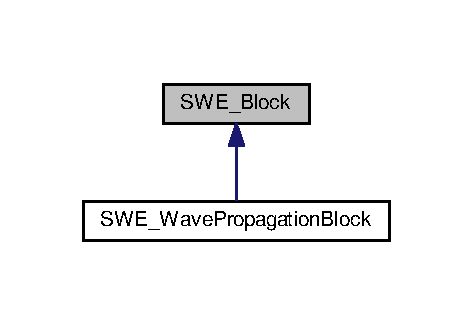
\includegraphics[width=227pt]{classSWE__Block__inherit__graph}
\end{center}
\end{figure}


Collaboration diagram for S\+W\+E\+\_\+\+Block\+:\nopagebreak
\begin{figure}[H]
\begin{center}
\leavevmode
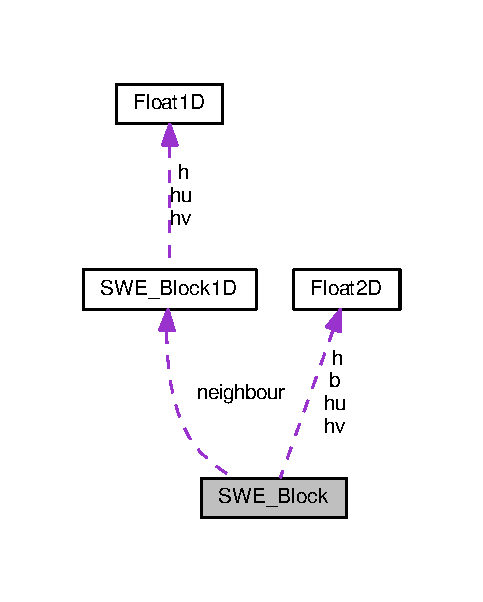
\includegraphics[width=232pt]{classSWE__Block__coll__graph}
\end{center}
\end{figure}
\subsection*{Public Member Functions}
\begin{DoxyCompactItemize}
\item 
void \hyperlink{classSWE__Block_a46b715c584468a5daa975ec1eb1ab947}{init\+Scenario} (float \+\_\+offsetX, float \+\_\+offsetY, \hyperlink{classSWE__Scenario}{S\+W\+E\+\_\+\+Scenario} \&i\+\_\+scenario, const bool i\+\_\+multiple\+Blocks=false)
\begin{DoxyCompactList}\small\item\em initialise unknowns to a specific scenario\+: \end{DoxyCompactList}\item 
void \hyperlink{classSWE__Block_a6481ce1c80a219fbefefdcbd13ed3688}{set\+Water\+Height} (float($\ast$\+\_\+h)(float, float))
\begin{DoxyCompactList}\small\item\em set the water height according to a given function \end{DoxyCompactList}\item 
void \hyperlink{classSWE__Block_a245332c325fd0ff6a7e9c2d3d9454970}{set\+Discharge} (float($\ast$\+\_\+u)(float, float), float($\ast$\+\_\+v)(float, float))
\begin{DoxyCompactList}\small\item\em set the momentum/discharge according to the provided functions \end{DoxyCompactList}\item 
void \hyperlink{classSWE__Block_af2ab34b138a14f2c295849f3b2acc5f3}{set\+Bathymetry} (float \+\_\+b)
\begin{DoxyCompactList}\small\item\em set the bathymetry to a uniform value \end{DoxyCompactList}\item 
void \hyperlink{classSWE__Block_ad4214fcfd102a4c167d274ad87d9dd90}{set\+Bathymetry} (float($\ast$\+\_\+b)(float, float))
\begin{DoxyCompactList}\small\item\em set the bathymetry according to a given function \end{DoxyCompactList}\item 
void \hyperlink{classSWE__Block_a215c50ff1bf0038cbeb90569593c5aa9}{set\+Water\+Height\+XY} (int x, int y, float h\+\_\+set)
\begin{DoxyCompactList}\small\item\em set a aditional wave with radius r and height h at x,y \end{DoxyCompactList}\item 
void \hyperlink{classSWE__Block_ab07678606e4d6e0331d91c014b4c0ad5}{set\+Bathymetry\+XY} (int x, int y, float h\+\_\+set)
\item 
void \hyperlink{classSWE__Block_ae9e24854137790c1e773ce7e08c8ccc9}{set\+Hu\+XY} (int x, int y, float h\+\_\+set)
\item 
void \hyperlink{classSWE__Block_a65153d7aeea996cc42045d28b0d05b5f}{set\+Hv\+XY} (int x, int y, float h\+\_\+set)
\item 
const \hyperlink{classFloat2D}{Float2D} \& \hyperlink{classSWE__Block_ab1aea4294403c194180c3dc107339fd7}{get\+Water\+Height} ()
\begin{DoxyCompactList}\small\item\em provides read access to the water height array \end{DoxyCompactList}\item 
const \hyperlink{classFloat2D}{Float2D} \& \hyperlink{classSWE__Block_ae5e766626a1e3fee89625610e2c67f1f}{get\+Discharge\+\_\+hu} ()
\begin{DoxyCompactList}\small\item\em provides read access to the momentum/discharge array (x-\/component) \end{DoxyCompactList}\item 
const \hyperlink{classFloat2D}{Float2D} \& \hyperlink{classSWE__Block_aece9e8dc3f9b8ab27420e537c76daf7c}{get\+Discharge\+\_\+hv} ()
\begin{DoxyCompactList}\small\item\em provides read access to the momentum/discharge array (y-\/component) \end{DoxyCompactList}\item 
const \hyperlink{classFloat2D}{Float2D} \& \hyperlink{classSWE__Block_a98e2c99a335d11d09a1489d6873b5615}{get\+Bathymetry} ()
\begin{DoxyCompactList}\small\item\em provides read access to the bathymetry data \end{DoxyCompactList}\item 
void \hyperlink{classSWE__Block_aa220b93e43b10f56c72a44d7363645c1}{set\+Boundary\+Type} (\hyperlink{scenarios_2SWE__Scenario_8hh_aa5e01e3f7df312f7b9b0d02521141fcc}{Boundary\+Edge} edge, \hyperlink{scenarios_2SWE__Scenario_8hh_af75d5dd7322fa39ed0af4e7839e600f8}{Boundary\+Type} boundtype, const \hyperlink{structSWE__Block1D}{S\+W\+E\+\_\+\+Block1D} $\ast$inflow=N\+U\+LL)
\begin{DoxyCompactList}\small\item\em set type of boundary condition for the specified boundary \end{DoxyCompactList}\item 
virtual \hyperlink{structSWE__Block1D}{S\+W\+E\+\_\+\+Block1D} $\ast$ \hyperlink{classSWE__Block_a827ee5c61dc9c1b472ac8b4e1c19956a}{register\+Copy\+Layer} (\hyperlink{scenarios_2SWE__Scenario_8hh_aa5e01e3f7df312f7b9b0d02521141fcc}{Boundary\+Edge} edge)
\begin{DoxyCompactList}\small\item\em return a pointer to proxy class to access the copy layer \end{DoxyCompactList}\item 
virtual \hyperlink{structSWE__Block1D}{S\+W\+E\+\_\+\+Block1D} $\ast$ \hyperlink{classSWE__Block_a9a96c59444645e237d098803009158a3}{grab\+Ghost\+Layer} (\hyperlink{scenarios_2SWE__Scenario_8hh_aa5e01e3f7df312f7b9b0d02521141fcc}{Boundary\+Edge} edge)
\begin{DoxyCompactList}\small\item\em \char`\"{}grab\char`\"{} the ghost layer in order to set these values externally \end{DoxyCompactList}\item 
void \hyperlink{classSWE__Block_afd17334abee3145e27cc3c9b7b935da2}{set\+Ghost\+Layer} ()
\begin{DoxyCompactList}\small\item\em set values in ghost layers \end{DoxyCompactList}\item 
float \hyperlink{classSWE__Block_a74da1eb712e639e47b5b848081b2afad}{get\+Max\+Timestep} ()
\begin{DoxyCompactList}\small\item\em return maximum size of the time step to ensure stability of the method \end{DoxyCompactList}\item 
void \hyperlink{classSWE__Block_acf2ff6617cbc0d3d837f0e618039cfe2}{compute\+Max\+Timestep} (const float i\+\_\+dry\+Tol=0.\+1, const float i\+\_\+cfl\+Number=0.\+4)
\item 
virtual void \hyperlink{classSWE__Block_add6908e1ceb261a0a1f3ebc262cc5f11}{simulate\+Timestep} (float dt)
\begin{DoxyCompactList}\small\item\em execute a single time step (with fixed time step size) of the simulation \end{DoxyCompactList}\item 
virtual float \hyperlink{classSWE__Block_a69784e2be2d09035fb2af9d306768f07}{simulate} (float t\+Start, float t\+End)
\item 
virtual void \hyperlink{classSWE__Block_a94dcf2c6ae31731e4586e45628b0c00e}{compute\+Numerical\+Fluxes} ()=0
\begin{DoxyCompactList}\small\item\em compute the numerical fluxes for each edge of the Cartesian grid \end{DoxyCompactList}\item 
virtual void \hyperlink{classSWE__Block_ab2b4b659f23d5d45413dece8d2da3298}{update\+Unknowns} (float dt)=0
\begin{DoxyCompactList}\small\item\em compute the new values of the unknowns h, hu, and hv in all grid cells \end{DoxyCompactList}\item 
int \hyperlink{classSWE__Block_aa27028fa4bc13bb2d9251b09e0fdfce6}{get\+Nx} ()
\begin{DoxyCompactList}\small\item\em returns \hyperlink{classSWE__Block_a46ec0dc1157997bd255fb39924f1e2bb}{nx}, i.\+e. the grid size in x-\/direction \end{DoxyCompactList}\item 
int \hyperlink{classSWE__Block_a4b65557b6f73ffb6454dad3dbf86e9ad}{get\+Ny} ()
\begin{DoxyCompactList}\small\item\em returns \hyperlink{classSWE__Block_a3f139630d12423eb4bd7df3e45c7f5da}{ny}, i.\+e. the grid size in y-\/direction \end{DoxyCompactList}\end{DoxyCompactItemize}
\subsection*{Static Public Attributes}
\begin{DoxyCompactItemize}
\item 
static const float \hyperlink{classSWE__Block_a073ca743ff4077a7e456906be704958f}{g} = 9.\+81f
\begin{DoxyCompactList}\small\item\em static variable that holds the gravity constant (g = 9.\+81 m/s$^\wedge$2)\+: \end{DoxyCompactList}\end{DoxyCompactItemize}
\subsection*{Protected Member Functions}
\begin{DoxyCompactItemize}
\item 
\hyperlink{classSWE__Block_a114ed3bb6a8a2c482e5f94f768543b82}{S\+W\+E\+\_\+\+Block} (int l\+\_\+nx, int l\+\_\+ny, float l\+\_\+dx, float l\+\_\+dy)
\item 
virtual \hyperlink{classSWE__Block_a2ddff1c284663ba514985a3574def1b0}{$\sim$\+S\+W\+E\+\_\+\+Block} ()
\item 
void \hyperlink{classSWE__Block_a6beb68dacde9c8479647c25c6a5cbcf5}{set\+Boundary\+Bathymetry} ()
\item 
virtual void \hyperlink{classSWE__Block_ae914f9bf6d4ef8f974f9f005114985e7}{synch\+After\+Write} ()
\item 
virtual void \hyperlink{classSWE__Block_aa2924833e29a795d8c04fb79bfe794de}{synch\+Water\+Height\+After\+Write} ()
\item 
virtual void \hyperlink{classSWE__Block_a94c34030153178c9d94f3f14be174eaf}{synch\+Discharge\+After\+Write} ()
\item 
virtual void \hyperlink{classSWE__Block_a4bece8aa90f67e55c40b91aab900febb}{synch\+Bathymetry\+After\+Write} ()
\item 
virtual void \hyperlink{classSWE__Block_a4657993ebdb5f0132b077e63790d0b2b}{synch\+Ghost\+Layer\+After\+Write} ()
\item 
virtual void \hyperlink{classSWE__Block_a23d936cb9a4367092e5b2515f81fe819}{synch\+Before\+Read} ()
\item 
virtual void \hyperlink{classSWE__Block_a07c85681ab29106c3b164db969899ace}{synch\+Water\+Height\+Before\+Read} ()
\item 
virtual void \hyperlink{classSWE__Block_a3773dcb194212fb8cb40ab8465575aa1}{synch\+Discharge\+Before\+Read} ()
\item 
virtual void \hyperlink{classSWE__Block_a7c8258c6949518ca44f4e9ce89d33b09}{synch\+Bathymetry\+Before\+Read} ()
\item 
virtual void \hyperlink{classSWE__Block_a13c90d5a6596336013c41e73c8795f83}{synch\+Copy\+Layer\+Before\+Read} ()
\item 
virtual void \hyperlink{classSWE__Block_a379807f0bf932b40aeb42065633fce60}{set\+Boundary\+Conditions} ()
\begin{DoxyCompactList}\small\item\em set boundary conditions in ghost layers (set boundary conditions) \end{DoxyCompactList}\end{DoxyCompactItemize}
\subsection*{Protected Attributes}
\begin{DoxyCompactItemize}
\item 
int \hyperlink{classSWE__Block_a46ec0dc1157997bd255fb39924f1e2bb}{nx}
\begin{DoxyCompactList}\small\item\em size of Cartesian arrays in x-\/direction \end{DoxyCompactList}\item 
int \hyperlink{classSWE__Block_a3f139630d12423eb4bd7df3e45c7f5da}{ny}
\begin{DoxyCompactList}\small\item\em size of Cartesian arrays in y-\/direction \end{DoxyCompactList}\item 
float \hyperlink{classSWE__Block_af2262b1cce6834d939c5a2315dae49b1}{dx}
\begin{DoxyCompactList}\small\item\em mesh size of the Cartesian grid in x-\/direction \end{DoxyCompactList}\item 
float \hyperlink{classSWE__Block_a9feb988748d792bca0ca0508e43bd87f}{dy}
\begin{DoxyCompactList}\small\item\em mesh size of the Cartesian grid in y-\/direction \end{DoxyCompactList}\item 
\hyperlink{classFloat2D}{Float2D} \hyperlink{classSWE__Block_a64a0f8f437f38b5f3b8ec5b4abdb864e}{h}
\begin{DoxyCompactList}\small\item\em array that holds the water height for each element \end{DoxyCompactList}\item 
\hyperlink{classFloat2D}{Float2D} \hyperlink{classSWE__Block_aec2c1278fdb23f083216d8d397f26060}{hu}
\begin{DoxyCompactList}\small\item\em array that holds the x-\/component of the momentum for each element (water height h multiplied by velocity in x-\/direction) \end{DoxyCompactList}\item 
\hyperlink{classFloat2D}{Float2D} \hyperlink{classSWE__Block_a0897aa3c2d78749f209c95e08196d831}{hv}
\begin{DoxyCompactList}\small\item\em array that holds the y-\/component of the momentum for each element (water height h multiplied by velocity in y-\/direction) \end{DoxyCompactList}\item 
\hyperlink{classFloat2D}{Float2D} \hyperlink{classSWE__Block_af7487209129f40b26ea171762754a261}{b}
\begin{DoxyCompactList}\small\item\em array that holds the bathymetry data (sea floor elevation) for each element \end{DoxyCompactList}\item 
\hyperlink{scenarios_2SWE__Scenario_8hh_af75d5dd7322fa39ed0af4e7839e600f8}{Boundary\+Type} \hyperlink{classSWE__Block_a0e56d0cad169abd4f5de95d9f96c7a73}{boundary} \mbox{[}4\mbox{]}
\begin{DoxyCompactList}\small\item\em type of boundary conditions at L\+E\+FT, R\+I\+G\+HT, T\+OP, and B\+O\+T\+T\+OM boundary \end{DoxyCompactList}\item 
const \hyperlink{structSWE__Block1D}{S\+W\+E\+\_\+\+Block1D} $\ast$ \hyperlink{classSWE__Block_a5ea4ea4815af9eb66c51de9ad9b8d148}{neighbour} \mbox{[}4\mbox{]}
\begin{DoxyCompactList}\small\item\em for C\+O\+N\+N\+E\+CT boundaries\+: pointer to connected neighbour block \end{DoxyCompactList}\item 
float \hyperlink{classSWE__Block_a05cbc9b40e0483bf73dbc2bdeae7dee3}{max\+Timestep}
\begin{DoxyCompactList}\small\item\em maximum time step allowed to ensure stability of the method \end{DoxyCompactList}\item 
float \hyperlink{classSWE__Block_aa9e9b1fa797c133c4989e4c54f09b542}{offsetX}
\begin{DoxyCompactList}\small\item\em x-\/coordinate of the origin (left-\/bottom corner) of the Cartesian grid \end{DoxyCompactList}\item 
float \hyperlink{classSWE__Block_aa05241101a66f0f0548eba6dbbaa1bbb}{offsetY}
\begin{DoxyCompactList}\small\item\em y-\/coordinate of the origin (left-\/bottom corner) of the Cartesian grid \end{DoxyCompactList}\end{DoxyCompactItemize}


\subsection{Detailed Description}
This file is part of S\+WE. 

\hyperlink{classSWE__Block}{S\+W\+E\+\_\+\+Block} is the main data structure to compute our shallow water model on a single Cartesian grid block\+: \hyperlink{classSWE__Block}{S\+W\+E\+\_\+\+Block} is an abstract class (and interface) that should be extended by respective implementation classes.

\paragraph*{Cartesian Grid for Discretization\+:}

S\+W\+E\+\_\+\+Blocks uses a regular Cartesian grid of size \hyperlink{classSWE__Block_a46ec0dc1157997bd255fb39924f1e2bb}{nx} by \hyperlink{classSWE__Block_a3f139630d12423eb4bd7df3e45c7f5da}{ny}, where each grid cell carries three unknowns\+:
\begin{DoxyItemize}
\item the water level \hyperlink{classSWE__Block_a64a0f8f437f38b5f3b8ec5b4abdb864e}{h}
\item the momentum components \hyperlink{classSWE__Block_aec2c1278fdb23f083216d8d397f26060}{hu} and \hyperlink{classSWE__Block_a0897aa3c2d78749f209c95e08196d831}{hv} (in x-\/ and y-\/ direction, resp.)
\item the bathymetry \hyperlink{classSWE__Block_af7487209129f40b26ea171762754a261}{b}
\end{DoxyItemize}

Each of the components is stored as a 2D array, implemented as a \hyperlink{classFloat2D}{Float2D} object, and are defined on grid indices \mbox{[}0,..,\hyperlink{classSWE__Block_a46ec0dc1157997bd255fb39924f1e2bb}{nx}+1\mbox{]}$\ast$\mbox{[}0,..,\hyperlink{classSWE__Block_a3f139630d12423eb4bd7df3e45c7f5da}{ny}+1\mbox{]}. The computational domain is indexed with \mbox{[}1,..,\hyperlink{classSWE__Block_a46ec0dc1157997bd255fb39924f1e2bb}{nx}\mbox{]}$\ast$\mbox{[}1,..,\hyperlink{classSWE__Block_a3f139630d12423eb4bd7df3e45c7f5da}{ny}\mbox{]}.

The mesh sizes of the grid in x-\/ and y-\/direction are stored in static variables \hyperlink{classSWE__Block_af2262b1cce6834d939c5a2315dae49b1}{dx} and \hyperlink{classSWE__Block_a9feb988748d792bca0ca0508e43bd87f}{dy}. The position of the Cartesian grid in space is stored via the coordinates of the left-\/bottom corner of the grid, in the variables \hyperlink{classSWE__Block_aa9e9b1fa797c133c4989e4c54f09b542}{offsetX} and \hyperlink{classSWE__Block_aa05241101a66f0f0548eba6dbbaa1bbb}{offsetY}.

\paragraph*{Ghost layers\+:}

To implement the behaviour of the fluid at boundaries and for using multiple block in serial and parallel settings, \hyperlink{classSWE__Block}{S\+W\+E\+\_\+\+Block} adds an additional layer of so-\/called ghost cells to the Cartesian grid, as illustrated in the following figure. Cells in the ghost layer have indices 0 or \hyperlink{classSWE__Block_a46ec0dc1157997bd255fb39924f1e2bb}{nx}+1 / \hyperlink{classSWE__Block_a3f139630d12423eb4bd7df3e45c7f5da}{ny}+1.



\paragraph*{Memory Model\+:}

The variables \hyperlink{classSWE__Block_a64a0f8f437f38b5f3b8ec5b4abdb864e}{h}, \hyperlink{classSWE__Block_aec2c1278fdb23f083216d8d397f26060}{hu}, \hyperlink{classSWE__Block_a0897aa3c2d78749f209c95e08196d831}{hv} for water height and momentum will typically be updated by classes derived from \hyperlink{classSWE__Block}{S\+W\+E\+\_\+\+Block}. However, it is not assumed that such and updated will be performed in every time step. Instead, subclasses are welcome to update \hyperlink{classSWE__Block_a64a0f8f437f38b5f3b8ec5b4abdb864e}{h}, \hyperlink{classSWE__Block_aec2c1278fdb23f083216d8d397f26060}{hu}, and \hyperlink{classSWE__Block_a0897aa3c2d78749f209c95e08196d831}{hv} in a lazy fashion, and keep data in faster memory (incl. local memory of acceleration hardware, such as G\+P\+G\+P\+Us), instead.

It is assumed that the bathymetry data \hyperlink{classSWE__Block_af7487209129f40b26ea171762754a261}{b} is not changed during the algorithm (up to the exceptions mentioned in the following).

To force a synchronization of the respective data structures, the following methods are provided as part of \hyperlink{classSWE__Block}{S\+W\+E\+\_\+\+Block}\+:
\begin{DoxyItemize}
\item \hyperlink{classSWE__Block_ae914f9bf6d4ef8f974f9f005114985e7}{synch\+After\+Write()} to synchronize \hyperlink{classSWE__Block_a64a0f8f437f38b5f3b8ec5b4abdb864e}{h}, \hyperlink{classSWE__Block_aec2c1278fdb23f083216d8d397f26060}{hu}, \hyperlink{classSWE__Block_a0897aa3c2d78749f209c95e08196d831}{hv}, and \hyperlink{classSWE__Block_af7487209129f40b26ea171762754a261}{b} after an external update (reading a file, e.\+g.);
\item \hyperlink{classSWE__Block_aa2924833e29a795d8c04fb79bfe794de}{synch\+Water\+Height\+After\+Write()}, \hyperlink{classSWE__Block_a94c34030153178c9d94f3f14be174eaf}{synch\+Discharge\+After\+Write()}, \hyperlink{classSWE__Block_a4bece8aa90f67e55c40b91aab900febb}{synch\+Bathymetry\+After\+Write()}\+: to synchronize only \hyperlink{classSWE__Block_a64a0f8f437f38b5f3b8ec5b4abdb864e}{h} or momentum (\hyperlink{classSWE__Block_aec2c1278fdb23f083216d8d397f26060}{hu} and \hyperlink{classSWE__Block_a0897aa3c2d78749f209c95e08196d831}{hv}) or bathymetry \hyperlink{classSWE__Block_af7487209129f40b26ea171762754a261}{b};
\item \hyperlink{classSWE__Block_a4657993ebdb5f0132b077e63790d0b2b}{synch\+Ghost\+Layer\+After\+Write()} to synchronize only the ghost layers
\item \hyperlink{classSWE__Block_a23d936cb9a4367092e5b2515f81fe819}{synch\+Before\+Read()} to synchronize \hyperlink{classSWE__Block_a64a0f8f437f38b5f3b8ec5b4abdb864e}{h}, \hyperlink{classSWE__Block_aec2c1278fdb23f083216d8d397f26060}{hu}, \hyperlink{classSWE__Block_a0897aa3c2d78749f209c95e08196d831}{hv}, and \hyperlink{classSWE__Block_af7487209129f40b26ea171762754a261}{b} before an output of the variables (writing a visualization file, e.\+g.)
\item \hyperlink{classSWE__Block_a07c85681ab29106c3b164db969899ace}{synch\+Water\+Height\+Before\+Read()}, \hyperlink{classSWE__Block_a3773dcb194212fb8cb40ab8465575aa1}{synch\+Discharge\+Before\+Read()}, \hyperlink{classSWE__Block_a7c8258c6949518ca44f4e9ce89d33b09}{synch\+Bathymetry\+Before\+Read()}\+: as \hyperlink{classSWE__Block_a23d936cb9a4367092e5b2515f81fe819}{synch\+Before\+Read()}, but only for the specified variables
\item \hyperlink{classSWE__Block_a13c90d5a6596336013c41e73c8795f83}{synch\+Copy\+Layer\+Before\+Read()}\+: synchronizes the copy layer only (i.\+e., a layer that is to be replicated in a neighbouring \hyperlink{classSWE__Block}{S\+W\+E\+\_\+\+Block}.
\end{DoxyItemize}

\paragraph*{Derived Classes}

As \hyperlink{classSWE__Block}{S\+W\+E\+\_\+\+Block} just provides an abstract base class together with the most important data structures, the implementation of concrete models is the job of respective derived classes (see the class diagram at the top of this page). Similar, parallel implementations that are based on a specific parallel programming model (such as Open\+MP) or parallel architecture (such as G\+P\+U/\+C\+U\+DA) should form subclasses of their own. Please refer to the documentation of these classes for more details on the model and on the parallelisation approach. 

Definition at line 115 of file S\+W\+E\+\_\+\+Block.\+hh.



\subsection{Constructor \& Destructor Documentation}
\index{S\+W\+E\+\_\+\+Block@{S\+W\+E\+\_\+\+Block}!S\+W\+E\+\_\+\+Block@{S\+W\+E\+\_\+\+Block}}
\index{S\+W\+E\+\_\+\+Block@{S\+W\+E\+\_\+\+Block}!S\+W\+E\+\_\+\+Block@{S\+W\+E\+\_\+\+Block}}
\subsubsection[{\texorpdfstring{S\+W\+E\+\_\+\+Block(int l\+\_\+nx, int l\+\_\+ny, float l\+\_\+dx, float l\+\_\+dy)}{SWE_Block(int l_nx, int l_ny, float l_dx, float l_dy)}}]{\setlength{\rightskip}{0pt plus 5cm}S\+W\+E\+\_\+\+Block\+::\+S\+W\+E\+\_\+\+Block (
\begin{DoxyParamCaption}
\item[{int}]{l\+\_\+nx, }
\item[{int}]{l\+\_\+ny, }
\item[{float}]{l\+\_\+dx, }
\item[{float}]{l\+\_\+dy}
\end{DoxyParamCaption}
)\hspace{0.3cm}{\ttfamily [protected]}}\hypertarget{classSWE__Block_a114ed3bb6a8a2c482e5f94f768543b82}{}\label{classSWE__Block_a114ed3bb6a8a2c482e5f94f768543b82}
Constructor\+: allocate variables for simulation

unknowns h (water height), hu,hv (discharge in x-\/ and y-\/direction), and b (bathymetry) are defined on grid indices \mbox{[}0,..,nx+1\mbox{]}$\ast$\mbox{[}0,..,ny+1\mbox{]} -\/$>$ computational domain is \mbox{[}1,..,nx\mbox{]}$\ast$\mbox{[}1,..,ny\mbox{]} -\/$>$ plus ghost cell layer

The constructor is protected\+: no instances of \hyperlink{classSWE__Block}{S\+W\+E\+\_\+\+Block} can be generated. 

Definition at line 52 of file S\+W\+E\+\_\+\+Block.\+cpp.

\index{S\+W\+E\+\_\+\+Block@{S\+W\+E\+\_\+\+Block}!````~S\+W\+E\+\_\+\+Block@{$\sim$\+S\+W\+E\+\_\+\+Block}}
\index{````~S\+W\+E\+\_\+\+Block@{$\sim$\+S\+W\+E\+\_\+\+Block}!S\+W\+E\+\_\+\+Block@{S\+W\+E\+\_\+\+Block}}
\subsubsection[{\texorpdfstring{$\sim$\+S\+W\+E\+\_\+\+Block()}{~SWE_Block()}}]{\setlength{\rightskip}{0pt plus 5cm}S\+W\+E\+\_\+\+Block\+::$\sim$\+S\+W\+E\+\_\+\+Block (
\begin{DoxyParamCaption}
{}
\end{DoxyParamCaption}
)\hspace{0.3cm}{\ttfamily [protected]}, {\ttfamily [virtual]}}\hypertarget{classSWE__Block_a2ddff1c284663ba514985a3574def1b0}{}\label{classSWE__Block_a2ddff1c284663ba514985a3574def1b0}
Destructor\+: de-\/allocate all variables 

Definition at line 70 of file S\+W\+E\+\_\+\+Block.\+cpp.



\subsection{Member Function Documentation}
\index{S\+W\+E\+\_\+\+Block@{S\+W\+E\+\_\+\+Block}!compute\+Max\+Timestep@{compute\+Max\+Timestep}}
\index{compute\+Max\+Timestep@{compute\+Max\+Timestep}!S\+W\+E\+\_\+\+Block@{S\+W\+E\+\_\+\+Block}}
\subsubsection[{\texorpdfstring{compute\+Max\+Timestep(const float i\+\_\+dry\+Tol=0.\+1, const float i\+\_\+cfl\+Number=0.\+4)}{computeMaxTimestep(const float i_dryTol=0.1, const float i_cflNumber=0.4)}}]{\setlength{\rightskip}{0pt plus 5cm}void S\+W\+E\+\_\+\+Block\+::compute\+Max\+Timestep (
\begin{DoxyParamCaption}
\item[{const float}]{i\+\_\+dry\+Tol = {\ttfamily 0.1}, }
\item[{const float}]{i\+\_\+cfl\+Number = {\ttfamily 0.4}}
\end{DoxyParamCaption}
)}\hypertarget{classSWE__Block_acf2ff6617cbc0d3d837f0e618039cfe2}{}\label{classSWE__Block_acf2ff6617cbc0d3d837f0e618039cfe2}
Compute the largest allowed time step for the current grid block (reference implementation) depending on the current values of variables h, hu, and hv, and store this time step size in member variable max\+Timestep.


\begin{DoxyParams}{Parameters}
{\em i\+\_\+dry\+Tol} & dry tolerance (dry cells do not affect the time step). \\
\hline
{\em i\+\_\+cfl\+Number} & C\+FL number of the used method. \\
\hline
\end{DoxyParams}


Definition at line 490 of file S\+W\+E\+\_\+\+Block.\+cpp.

\index{S\+W\+E\+\_\+\+Block@{S\+W\+E\+\_\+\+Block}!compute\+Numerical\+Fluxes@{compute\+Numerical\+Fluxes}}
\index{compute\+Numerical\+Fluxes@{compute\+Numerical\+Fluxes}!S\+W\+E\+\_\+\+Block@{S\+W\+E\+\_\+\+Block}}
\subsubsection[{\texorpdfstring{compute\+Numerical\+Fluxes()=0}{computeNumericalFluxes()=0}}]{\setlength{\rightskip}{0pt plus 5cm}virtual void S\+W\+E\+\_\+\+Block\+::compute\+Numerical\+Fluxes (
\begin{DoxyParamCaption}
{}
\end{DoxyParamCaption}
)\hspace{0.3cm}{\ttfamily [pure virtual]}}\hypertarget{classSWE__Block_a94dcf2c6ae31731e4586e45628b0c00e}{}\label{classSWE__Block_a94dcf2c6ae31731e4586e45628b0c00e}


compute the numerical fluxes for each edge of the Cartesian grid 

The computation of fluxes strongly depends on the chosen numerical method. Hence, this purely virtual function has to be implemented in the respective derived classes. 

Implemented in \hyperlink{classSWE__WavePropagationBlock_a5f6335a38fb3cf38623326959f06baf4}{S\+W\+E\+\_\+\+Wave\+Propagation\+Block}.

\index{S\+W\+E\+\_\+\+Block@{S\+W\+E\+\_\+\+Block}!get\+Bathymetry@{get\+Bathymetry}}
\index{get\+Bathymetry@{get\+Bathymetry}!S\+W\+E\+\_\+\+Block@{S\+W\+E\+\_\+\+Block}}
\subsubsection[{\texorpdfstring{get\+Bathymetry()}{getBathymetry()}}]{\setlength{\rightskip}{0pt plus 5cm}const {\bf Float2D} \& S\+W\+E\+\_\+\+Block\+::get\+Bathymetry (
\begin{DoxyParamCaption}
{}
\end{DoxyParamCaption}
)}\hypertarget{classSWE__Block_a98e2c99a335d11d09a1489d6873b5615}{}\label{classSWE__Block_a98e2c99a335d11d09a1489d6873b5615}


provides read access to the bathymetry data 

return reference to bathymetry unknown b 

Definition at line 259 of file S\+W\+E\+\_\+\+Block.\+cpp.

\index{S\+W\+E\+\_\+\+Block@{S\+W\+E\+\_\+\+Block}!get\+Discharge\+\_\+hu@{get\+Discharge\+\_\+hu}}
\index{get\+Discharge\+\_\+hu@{get\+Discharge\+\_\+hu}!S\+W\+E\+\_\+\+Block@{S\+W\+E\+\_\+\+Block}}
\subsubsection[{\texorpdfstring{get\+Discharge\+\_\+hu()}{getDischarge_hu()}}]{\setlength{\rightskip}{0pt plus 5cm}const {\bf Float2D} \& S\+W\+E\+\_\+\+Block\+::get\+Discharge\+\_\+hu (
\begin{DoxyParamCaption}
{}
\end{DoxyParamCaption}
)}\hypertarget{classSWE__Block_ae5e766626a1e3fee89625610e2c67f1f}{}\label{classSWE__Block_ae5e766626a1e3fee89625610e2c67f1f}


provides read access to the momentum/discharge array (x-\/component) 

return reference to discharge unknown hu 

Definition at line 243 of file S\+W\+E\+\_\+\+Block.\+cpp.

\index{S\+W\+E\+\_\+\+Block@{S\+W\+E\+\_\+\+Block}!get\+Discharge\+\_\+hv@{get\+Discharge\+\_\+hv}}
\index{get\+Discharge\+\_\+hv@{get\+Discharge\+\_\+hv}!S\+W\+E\+\_\+\+Block@{S\+W\+E\+\_\+\+Block}}
\subsubsection[{\texorpdfstring{get\+Discharge\+\_\+hv()}{getDischarge_hv()}}]{\setlength{\rightskip}{0pt plus 5cm}const {\bf Float2D} \& S\+W\+E\+\_\+\+Block\+::get\+Discharge\+\_\+hv (
\begin{DoxyParamCaption}
{}
\end{DoxyParamCaption}
)}\hypertarget{classSWE__Block_aece9e8dc3f9b8ab27420e537c76daf7c}{}\label{classSWE__Block_aece9e8dc3f9b8ab27420e537c76daf7c}


provides read access to the momentum/discharge array (y-\/component) 

return reference to discharge unknown hv 

Definition at line 251 of file S\+W\+E\+\_\+\+Block.\+cpp.

\index{S\+W\+E\+\_\+\+Block@{S\+W\+E\+\_\+\+Block}!get\+Max\+Timestep@{get\+Max\+Timestep}}
\index{get\+Max\+Timestep@{get\+Max\+Timestep}!S\+W\+E\+\_\+\+Block@{S\+W\+E\+\_\+\+Block}}
\subsubsection[{\texorpdfstring{get\+Max\+Timestep()}{getMaxTimestep()}}]{\setlength{\rightskip}{0pt plus 5cm}float S\+W\+E\+\_\+\+Block\+::get\+Max\+Timestep (
\begin{DoxyParamCaption}
{}
\end{DoxyParamCaption}
)\hspace{0.3cm}{\ttfamily [inline]}}\hypertarget{classSWE__Block_a74da1eb712e639e47b5b848081b2afad}{}\label{classSWE__Block_a74da1eb712e639e47b5b848081b2afad}


return maximum size of the time step to ensure stability of the method 

\begin{DoxyReturn}{Returns}
current value of the member variable \hyperlink{classSWE__Block_a05cbc9b40e0483bf73dbc2bdeae7dee3}{max\+Timestep} 
\end{DoxyReturn}


Definition at line 166 of file S\+W\+E\+\_\+\+Block.\+hh.

\index{S\+W\+E\+\_\+\+Block@{S\+W\+E\+\_\+\+Block}!get\+Nx@{get\+Nx}}
\index{get\+Nx@{get\+Nx}!S\+W\+E\+\_\+\+Block@{S\+W\+E\+\_\+\+Block}}
\subsubsection[{\texorpdfstring{get\+Nx()}{getNx()}}]{\setlength{\rightskip}{0pt plus 5cm}int S\+W\+E\+\_\+\+Block\+::get\+Nx (
\begin{DoxyParamCaption}
{}
\end{DoxyParamCaption}
)\hspace{0.3cm}{\ttfamily [inline]}}\hypertarget{classSWE__Block_aa27028fa4bc13bb2d9251b09e0fdfce6}{}\label{classSWE__Block_aa27028fa4bc13bb2d9251b09e0fdfce6}


returns \hyperlink{classSWE__Block_a46ec0dc1157997bd255fb39924f1e2bb}{nx}, i.\+e. the grid size in x-\/direction 



Definition at line 199 of file S\+W\+E\+\_\+\+Block.\+hh.

\index{S\+W\+E\+\_\+\+Block@{S\+W\+E\+\_\+\+Block}!get\+Ny@{get\+Ny}}
\index{get\+Ny@{get\+Ny}!S\+W\+E\+\_\+\+Block@{S\+W\+E\+\_\+\+Block}}
\subsubsection[{\texorpdfstring{get\+Ny()}{getNy()}}]{\setlength{\rightskip}{0pt plus 5cm}int S\+W\+E\+\_\+\+Block\+::get\+Ny (
\begin{DoxyParamCaption}
{}
\end{DoxyParamCaption}
)\hspace{0.3cm}{\ttfamily [inline]}}\hypertarget{classSWE__Block_a4b65557b6f73ffb6454dad3dbf86e9ad}{}\label{classSWE__Block_a4b65557b6f73ffb6454dad3dbf86e9ad}


returns \hyperlink{classSWE__Block_a3f139630d12423eb4bd7df3e45c7f5da}{ny}, i.\+e. the grid size in y-\/direction 



Definition at line 201 of file S\+W\+E\+\_\+\+Block.\+hh.

\index{S\+W\+E\+\_\+\+Block@{S\+W\+E\+\_\+\+Block}!get\+Water\+Height@{get\+Water\+Height}}
\index{get\+Water\+Height@{get\+Water\+Height}!S\+W\+E\+\_\+\+Block@{S\+W\+E\+\_\+\+Block}}
\subsubsection[{\texorpdfstring{get\+Water\+Height()}{getWaterHeight()}}]{\setlength{\rightskip}{0pt plus 5cm}const {\bf Float2D} \& S\+W\+E\+\_\+\+Block\+::get\+Water\+Height (
\begin{DoxyParamCaption}
{}
\end{DoxyParamCaption}
)}\hypertarget{classSWE__Block_ab1aea4294403c194180c3dc107339fd7}{}\label{classSWE__Block_ab1aea4294403c194180c3dc107339fd7}


provides read access to the water height array 

Restores values for h, v, and u from file data 
\begin{DoxyParams}{Parameters}
{\em \+\_\+b} & array holding b-\/values in sequence return reference to water height unknown h \\
\hline
\end{DoxyParams}


Definition at line 235 of file S\+W\+E\+\_\+\+Block.\+cpp.

\index{S\+W\+E\+\_\+\+Block@{S\+W\+E\+\_\+\+Block}!grab\+Ghost\+Layer@{grab\+Ghost\+Layer}}
\index{grab\+Ghost\+Layer@{grab\+Ghost\+Layer}!S\+W\+E\+\_\+\+Block@{S\+W\+E\+\_\+\+Block}}
\subsubsection[{\texorpdfstring{grab\+Ghost\+Layer(\+Boundary\+Edge edge)}{grabGhostLayer(BoundaryEdge edge)}}]{\setlength{\rightskip}{0pt plus 5cm}{\bf S\+W\+E\+\_\+\+Block1D} $\ast$ S\+W\+E\+\_\+\+Block\+::grab\+Ghost\+Layer (
\begin{DoxyParamCaption}
\item[{{\bf Boundary\+Edge}}]{edge}
\end{DoxyParamCaption}
)\hspace{0.3cm}{\ttfamily [virtual]}}\hypertarget{classSWE__Block_a9a96c59444645e237d098803009158a3}{}\label{classSWE__Block_a9a96c59444645e237d098803009158a3}


\char`\"{}grab\char`\"{} the ghost layer in order to set these values externally 

\char`\"{}grab\char`\"{} the ghost layer at the specific boundary in order to set boundary values in this ghost layer externally. The boundary conditions at the respective ghost layer is set to P\+A\+S\+S\+I\+VE, such that the grabbing program component is responsible to provide correct values in the ghost layer, for example by receiving data from a remote copy layer via M\+PI communication. 
\begin{DoxyParams}{Parameters}
{\em specified} & edge \\
\hline
\end{DoxyParams}
\begin{DoxyReturn}{Returns}
a \hyperlink{structSWE__Block1D}{S\+W\+E\+\_\+\+Block1D} object that contains row variables h, hu, and hv 
\end{DoxyReturn}


Definition at line 398 of file S\+W\+E\+\_\+\+Block.\+cpp.

\index{S\+W\+E\+\_\+\+Block@{S\+W\+E\+\_\+\+Block}!init\+Scenario@{init\+Scenario}}
\index{init\+Scenario@{init\+Scenario}!S\+W\+E\+\_\+\+Block@{S\+W\+E\+\_\+\+Block}}
\subsubsection[{\texorpdfstring{init\+Scenario(float \+\_\+offset\+X, float \+\_\+offset\+Y, S\+W\+E\+\_\+\+Scenario \&i\+\_\+scenario, const bool i\+\_\+multiple\+Blocks=false)}{initScenario(float _offsetX, float _offsetY, SWE_Scenario &i_scenario, const bool i_multipleBlocks=false)}}]{\setlength{\rightskip}{0pt plus 5cm}void S\+W\+E\+\_\+\+Block\+::init\+Scenario (
\begin{DoxyParamCaption}
\item[{float}]{\+\_\+offsetX, }
\item[{float}]{\+\_\+offsetY, }
\item[{{\bf S\+W\+E\+\_\+\+Scenario} \&}]{i\+\_\+scenario, }
\item[{const bool}]{i\+\_\+multiple\+Blocks = {\ttfamily false}}
\end{DoxyParamCaption}
)}\hypertarget{classSWE__Block_a46b715c584468a5daa975ec1eb1ab947}{}\label{classSWE__Block_a46b715c584468a5daa975ec1eb1ab947}


initialise unknowns to a specific scenario\+: 

Initializes the unknowns and bathymetry in all grid cells according to the given \hyperlink{classSWE__Scenario}{S\+W\+E\+\_\+\+Scenario}.

In the case of multiple S\+W\+E\+\_\+\+Blocks at this point, it is not clear how the boundary conditions should be set. This is because an isolated \hyperlink{classSWE__Block}{S\+W\+E\+\_\+\+Block} doesn\textquotesingle{}t have any in information about the grid. Therefore the calling routine, which has the information about multiple blocks, has to take care about setting the right boundary conditions.


\begin{DoxyParams}{Parameters}
{\em i\+\_\+scenario} & scenario, which is used during the setup. \\
\hline
{\em i\+\_\+multiple\+Blocks} & are the multiple S\+W\+E\+\_\+blocks? \\
\hline
\end{DoxyParams}


Definition at line 90 of file S\+W\+E\+\_\+\+Block.\+cpp.

\index{S\+W\+E\+\_\+\+Block@{S\+W\+E\+\_\+\+Block}!register\+Copy\+Layer@{register\+Copy\+Layer}}
\index{register\+Copy\+Layer@{register\+Copy\+Layer}!S\+W\+E\+\_\+\+Block@{S\+W\+E\+\_\+\+Block}}
\subsubsection[{\texorpdfstring{register\+Copy\+Layer(\+Boundary\+Edge edge)}{registerCopyLayer(BoundaryEdge edge)}}]{\setlength{\rightskip}{0pt plus 5cm}{\bf S\+W\+E\+\_\+\+Block1D} $\ast$ S\+W\+E\+\_\+\+Block\+::register\+Copy\+Layer (
\begin{DoxyParamCaption}
\item[{{\bf Boundary\+Edge}}]{edge}
\end{DoxyParamCaption}
)\hspace{0.3cm}{\ttfamily [virtual]}}\hypertarget{classSWE__Block_a827ee5c61dc9c1b472ac8b4e1c19956a}{}\label{classSWE__Block_a827ee5c61dc9c1b472ac8b4e1c19956a}


return a pointer to proxy class to access the copy layer 

register the row or column layer next to a boundary as a \char`\"{}copy layer\char`\"{}, from which values will be copied into the ghost layer or a neighbour; \begin{DoxyReturn}{Returns}
a \hyperlink{structSWE__Block1D}{S\+W\+E\+\_\+\+Block1D} object that contains row variables h, hu, and hv 
\end{DoxyReturn}


Definition at line 373 of file S\+W\+E\+\_\+\+Block.\+cpp.

\index{S\+W\+E\+\_\+\+Block@{S\+W\+E\+\_\+\+Block}!set\+Bathymetry@{set\+Bathymetry}}
\index{set\+Bathymetry@{set\+Bathymetry}!S\+W\+E\+\_\+\+Block@{S\+W\+E\+\_\+\+Block}}
\subsubsection[{\texorpdfstring{set\+Bathymetry(float \+\_\+b)}{setBathymetry(float _b)}}]{\setlength{\rightskip}{0pt plus 5cm}void S\+W\+E\+\_\+\+Block\+::set\+Bathymetry (
\begin{DoxyParamCaption}
\item[{float}]{\+\_\+b}
\end{DoxyParamCaption}
)}\hypertarget{classSWE__Block_af2ab34b138a14f2c295849f3b2acc5f3}{}\label{classSWE__Block_af2ab34b138a14f2c295849f3b2acc5f3}


set the bathymetry to a uniform value 

set Bathymetry b in all grid cells (incl. ghost/boundary layers) to a uniform value bathymetry source terms are re-\/computed 

Definition at line 179 of file S\+W\+E\+\_\+\+Block.\+cpp.

\index{S\+W\+E\+\_\+\+Block@{S\+W\+E\+\_\+\+Block}!set\+Bathymetry@{set\+Bathymetry}}
\index{set\+Bathymetry@{set\+Bathymetry}!S\+W\+E\+\_\+\+Block@{S\+W\+E\+\_\+\+Block}}
\subsubsection[{\texorpdfstring{set\+Bathymetry(float($\ast$\+\_\+b)(float, float))}{setBathymetry(float(*_b)(float, float))}}]{\setlength{\rightskip}{0pt plus 5cm}void S\+W\+E\+\_\+\+Block\+::set\+Bathymetry (
\begin{DoxyParamCaption}
\item[{float($\ast$)(float, float)}]{\+\_\+b}
\end{DoxyParamCaption}
)}\hypertarget{classSWE__Block_ad4214fcfd102a4c167d274ad87d9dd90}{}\label{classSWE__Block_ad4214fcfd102a4c167d274ad87d9dd90}


set the bathymetry according to a given function 

set Bathymetry b in all grid cells (incl. ghost/boundary layers) using the specified bathymetry function; bathymetry source terms are re-\/computed 

Definition at line 193 of file S\+W\+E\+\_\+\+Block.\+cpp.

\index{S\+W\+E\+\_\+\+Block@{S\+W\+E\+\_\+\+Block}!set\+Bathymetry\+XY@{set\+Bathymetry\+XY}}
\index{set\+Bathymetry\+XY@{set\+Bathymetry\+XY}!S\+W\+E\+\_\+\+Block@{S\+W\+E\+\_\+\+Block}}
\subsubsection[{\texorpdfstring{set\+Bathymetry\+X\+Y(int x, int y, float h\+\_\+set)}{setBathymetryXY(int x, int y, float h_set)}}]{\setlength{\rightskip}{0pt plus 5cm}void S\+W\+E\+\_\+\+Block\+::set\+Bathymetry\+XY (
\begin{DoxyParamCaption}
\item[{int}]{x, }
\item[{int}]{y, }
\item[{float}]{h\+\_\+set}
\end{DoxyParamCaption}
)}\hypertarget{classSWE__Block_ab07678606e4d6e0331d91c014b4c0ad5}{}\label{classSWE__Block_ab07678606e4d6e0331d91c014b4c0ad5}


Definition at line 131 of file S\+W\+E\+\_\+\+Block.\+cpp.

\index{S\+W\+E\+\_\+\+Block@{S\+W\+E\+\_\+\+Block}!set\+Boundary\+Bathymetry@{set\+Boundary\+Bathymetry}}
\index{set\+Boundary\+Bathymetry@{set\+Boundary\+Bathymetry}!S\+W\+E\+\_\+\+Block@{S\+W\+E\+\_\+\+Block}}
\subsubsection[{\texorpdfstring{set\+Boundary\+Bathymetry()}{setBoundaryBathymetry()}}]{\setlength{\rightskip}{0pt plus 5cm}void S\+W\+E\+\_\+\+Block\+::set\+Boundary\+Bathymetry (
\begin{DoxyParamCaption}
{}
\end{DoxyParamCaption}
)\hspace{0.3cm}{\ttfamily [protected]}}\hypertarget{classSWE__Block_a6beb68dacde9c8479647c25c6a5cbcf5}{}\label{classSWE__Block_a6beb68dacde9c8479647c25c6a5cbcf5}
Sets the bathymetry on O\+U\+T\+F\+L\+OW or W\+A\+LL boundaries. Should be called very time a boundary is changed to a O\+U\+T\+F\+L\+OW or W\+A\+LL boundary {\bfseries or} the bathymetry changes. 

Definition at line 337 of file S\+W\+E\+\_\+\+Block.\+cpp.

\index{S\+W\+E\+\_\+\+Block@{S\+W\+E\+\_\+\+Block}!set\+Boundary\+Conditions@{set\+Boundary\+Conditions}}
\index{set\+Boundary\+Conditions@{set\+Boundary\+Conditions}!S\+W\+E\+\_\+\+Block@{S\+W\+E\+\_\+\+Block}}
\subsubsection[{\texorpdfstring{set\+Boundary\+Conditions()}{setBoundaryConditions()}}]{\setlength{\rightskip}{0pt plus 5cm}void S\+W\+E\+\_\+\+Block\+::set\+Boundary\+Conditions (
\begin{DoxyParamCaption}
{}
\end{DoxyParamCaption}
)\hspace{0.3cm}{\ttfamily [protected]}, {\ttfamily [virtual]}}\hypertarget{classSWE__Block_a379807f0bf932b40aeb42065633fce60}{}\label{classSWE__Block_a379807f0bf932b40aeb42065633fce60}


set boundary conditions in ghost layers (set boundary conditions) 

set the values of all ghost cells depending on the specifed boundary conditions
\begin{DoxyItemize}
\item set boundary conditions for typs W\+A\+LL and O\+U\+T\+F\+L\+OW
\item derived classes need to transfer ghost layers 
\end{DoxyItemize}

Definition at line 534 of file S\+W\+E\+\_\+\+Block.\+cpp.

\index{S\+W\+E\+\_\+\+Block@{S\+W\+E\+\_\+\+Block}!set\+Boundary\+Type@{set\+Boundary\+Type}}
\index{set\+Boundary\+Type@{set\+Boundary\+Type}!S\+W\+E\+\_\+\+Block@{S\+W\+E\+\_\+\+Block}}
\subsubsection[{\texorpdfstring{set\+Boundary\+Type(\+Boundary\+Edge edge, Boundary\+Type boundtype, const S\+W\+E\+\_\+\+Block1\+D $\ast$inflow=\+N\+U\+L\+L)}{setBoundaryType(BoundaryEdge edge, BoundaryType boundtype, const SWE_Block1D *inflow=NULL)}}]{\setlength{\rightskip}{0pt plus 5cm}void S\+W\+E\+\_\+\+Block\+::set\+Boundary\+Type (
\begin{DoxyParamCaption}
\item[{{\bf Boundary\+Edge}}]{edge, }
\item[{{\bf Boundary\+Type}}]{boundtype, }
\item[{const {\bf S\+W\+E\+\_\+\+Block1D} $\ast$}]{i\+\_\+inflow = {\ttfamily NULL}}
\end{DoxyParamCaption}
)}\hypertarget{classSWE__Block_aa220b93e43b10f56c72a44d7363645c1}{}\label{classSWE__Block_aa220b93e43b10f56c72a44d7363645c1}


set type of boundary condition for the specified boundary 

Set the boundary type for specific block boundary.


\begin{DoxyParams}{Parameters}
{\em i\+\_\+edge} & location of the edge relative to the S\+W\+E\+\_\+block. \\
\hline
{\em i\+\_\+boundary\+Type} & type of the boundary condition. \\
\hline
{\em i\+\_\+inflow} & pointer to an \hyperlink{structSWE__Block1D}{S\+W\+E\+\_\+\+Block1D}, which specifies the inflow (should be N\+U\+LL for W\+A\+LL or O\+U\+T\+F\+L\+OW boundary) \\
\hline
\end{DoxyParams}


Definition at line 320 of file S\+W\+E\+\_\+\+Block.\+cpp.

\index{S\+W\+E\+\_\+\+Block@{S\+W\+E\+\_\+\+Block}!set\+Discharge@{set\+Discharge}}
\index{set\+Discharge@{set\+Discharge}!S\+W\+E\+\_\+\+Block@{S\+W\+E\+\_\+\+Block}}
\subsubsection[{\texorpdfstring{set\+Discharge(float($\ast$\+\_\+u)(float, float), float($\ast$\+\_\+v)(float, float))}{setDischarge(float(*_u)(float, float), float(*_v)(float, float))}}]{\setlength{\rightskip}{0pt plus 5cm}void S\+W\+E\+\_\+\+Block\+::set\+Discharge (
\begin{DoxyParamCaption}
\item[{float($\ast$)(float, float)}]{\+\_\+u, }
\item[{float($\ast$)(float, float)}]{\+\_\+v}
\end{DoxyParamCaption}
)}\hypertarget{classSWE__Block_a245332c325fd0ff6a7e9c2d3d9454970}{}\label{classSWE__Block_a245332c325fd0ff6a7e9c2d3d9454970}


set the momentum/discharge according to the provided functions 

set discharge in all interior grid cells (i.\+e. except ghost layer) to values specified by parameter functions Note\+: unknowns hu and hv represent momentum, while parameters u and v are velocities! 

Definition at line 161 of file S\+W\+E\+\_\+\+Block.\+cpp.

\index{S\+W\+E\+\_\+\+Block@{S\+W\+E\+\_\+\+Block}!set\+Ghost\+Layer@{set\+Ghost\+Layer}}
\index{set\+Ghost\+Layer@{set\+Ghost\+Layer}!S\+W\+E\+\_\+\+Block@{S\+W\+E\+\_\+\+Block}}
\subsubsection[{\texorpdfstring{set\+Ghost\+Layer()}{setGhostLayer()}}]{\setlength{\rightskip}{0pt plus 5cm}void S\+W\+E\+\_\+\+Block\+::set\+Ghost\+Layer (
\begin{DoxyParamCaption}
{}
\end{DoxyParamCaption}
)}\hypertarget{classSWE__Block_afd17334abee3145e27cc3c9b7b935da2}{}\label{classSWE__Block_afd17334abee3145e27cc3c9b7b935da2}


set values in ghost layers 

set the values of all ghost cells depending on the specifed boundary conditions; if the ghost layer replicates the variables of a remote \hyperlink{classSWE__Block}{S\+W\+E\+\_\+\+Block}, the values are copied 

Definition at line 421 of file S\+W\+E\+\_\+\+Block.\+cpp.

\index{S\+W\+E\+\_\+\+Block@{S\+W\+E\+\_\+\+Block}!set\+Hu\+XY@{set\+Hu\+XY}}
\index{set\+Hu\+XY@{set\+Hu\+XY}!S\+W\+E\+\_\+\+Block@{S\+W\+E\+\_\+\+Block}}
\subsubsection[{\texorpdfstring{set\+Hu\+X\+Y(int x, int y, float h\+\_\+set)}{setHuXY(int x, int y, float h_set)}}]{\setlength{\rightskip}{0pt plus 5cm}void S\+W\+E\+\_\+\+Block\+::set\+Hu\+XY (
\begin{DoxyParamCaption}
\item[{int}]{x, }
\item[{int}]{y, }
\item[{float}]{h\+\_\+set}
\end{DoxyParamCaption}
)}\hypertarget{classSWE__Block_ae9e24854137790c1e773ce7e08c8ccc9}{}\label{classSWE__Block_ae9e24854137790c1e773ce7e08c8ccc9}


Definition at line 135 of file S\+W\+E\+\_\+\+Block.\+cpp.

\index{S\+W\+E\+\_\+\+Block@{S\+W\+E\+\_\+\+Block}!set\+Hv\+XY@{set\+Hv\+XY}}
\index{set\+Hv\+XY@{set\+Hv\+XY}!S\+W\+E\+\_\+\+Block@{S\+W\+E\+\_\+\+Block}}
\subsubsection[{\texorpdfstring{set\+Hv\+X\+Y(int x, int y, float h\+\_\+set)}{setHvXY(int x, int y, float h_set)}}]{\setlength{\rightskip}{0pt plus 5cm}void S\+W\+E\+\_\+\+Block\+::set\+Hv\+XY (
\begin{DoxyParamCaption}
\item[{int}]{x, }
\item[{int}]{y, }
\item[{float}]{h\+\_\+set}
\end{DoxyParamCaption}
)}\hypertarget{classSWE__Block_a65153d7aeea996cc42045d28b0d05b5f}{}\label{classSWE__Block_a65153d7aeea996cc42045d28b0d05b5f}


Definition at line 139 of file S\+W\+E\+\_\+\+Block.\+cpp.

\index{S\+W\+E\+\_\+\+Block@{S\+W\+E\+\_\+\+Block}!set\+Water\+Height@{set\+Water\+Height}}
\index{set\+Water\+Height@{set\+Water\+Height}!S\+W\+E\+\_\+\+Block@{S\+W\+E\+\_\+\+Block}}
\subsubsection[{\texorpdfstring{set\+Water\+Height(float($\ast$\+\_\+h)(float, float))}{setWaterHeight(float(*_h)(float, float))}}]{\setlength{\rightskip}{0pt plus 5cm}void S\+W\+E\+\_\+\+Block\+::set\+Water\+Height (
\begin{DoxyParamCaption}
\item[{float($\ast$)(float, float)}]{\+\_\+h}
\end{DoxyParamCaption}
)}\hypertarget{classSWE__Block_a6481ce1c80a219fbefefdcbd13ed3688}{}\label{classSWE__Block_a6481ce1c80a219fbefefdcbd13ed3688}


set the water height according to a given function 

set water height h in all interior grid cells (i.\+e. except ghost layer) to values specified by parameter function \+\_\+h 

Definition at line 147 of file S\+W\+E\+\_\+\+Block.\+cpp.

\index{S\+W\+E\+\_\+\+Block@{S\+W\+E\+\_\+\+Block}!set\+Water\+Height\+XY@{set\+Water\+Height\+XY}}
\index{set\+Water\+Height\+XY@{set\+Water\+Height\+XY}!S\+W\+E\+\_\+\+Block@{S\+W\+E\+\_\+\+Block}}
\subsubsection[{\texorpdfstring{set\+Water\+Height\+X\+Y(int x, int y, float h\+\_\+set)}{setWaterHeightXY(int x, int y, float h_set)}}]{\setlength{\rightskip}{0pt plus 5cm}void S\+W\+E\+\_\+\+Block\+::set\+Water\+Height\+XY (
\begin{DoxyParamCaption}
\item[{int}]{x, }
\item[{int}]{y, }
\item[{float}]{h\+\_\+set}
\end{DoxyParamCaption}
)}\hypertarget{classSWE__Block_a215c50ff1bf0038cbeb90569593c5aa9}{}\label{classSWE__Block_a215c50ff1bf0038cbeb90569593c5aa9}


set a aditional wave with radius r and height h at x,y 



Definition at line 127 of file S\+W\+E\+\_\+\+Block.\+cpp.

\index{S\+W\+E\+\_\+\+Block@{S\+W\+E\+\_\+\+Block}!simulate@{simulate}}
\index{simulate@{simulate}!S\+W\+E\+\_\+\+Block@{S\+W\+E\+\_\+\+Block}}
\subsubsection[{\texorpdfstring{simulate(float t\+Start, float t\+End)}{simulate(float tStart, float tEnd)}}]{\setlength{\rightskip}{0pt plus 5cm}float S\+W\+E\+\_\+\+Block\+::simulate (
\begin{DoxyParamCaption}
\item[{float}]{i\+\_\+t\+Start, }
\item[{float}]{i\+\_\+t\+End}
\end{DoxyParamCaption}
)\hspace{0.3cm}{\ttfamily [virtual]}}\hypertarget{classSWE__Block_a69784e2be2d09035fb2af9d306768f07}{}\label{classSWE__Block_a69784e2be2d09035fb2af9d306768f07}
perform the simulation starting with simulation time t\+Start, until simulation time t\+End is reached

simulate implements the main simulation loop between two checkpoints; Note\+: this implementation can only be used, if you only use a single \hyperlink{classSWE__Block}{S\+W\+E\+\_\+\+Block} and only apply simple boundary conditions! In particular, \hyperlink{classSWE__Block_a69784e2be2d09035fb2af9d306768f07}{S\+W\+E\+\_\+\+Block\+::simulate} can not trigger calls to exchange values of copy and ghost layers between blocks! 
\begin{DoxyParams}{Parameters}
{\em t\+Start} & time where the simulation is started \\
\hline
{\em t\+End} & time of the next checkpoint \\
\hline
\end{DoxyParams}
\begin{DoxyReturn}{Returns}
actual end time reached 
\end{DoxyReturn}


Definition at line 293 of file S\+W\+E\+\_\+\+Block.\+cpp.

\index{S\+W\+E\+\_\+\+Block@{S\+W\+E\+\_\+\+Block}!simulate\+Timestep@{simulate\+Timestep}}
\index{simulate\+Timestep@{simulate\+Timestep}!S\+W\+E\+\_\+\+Block@{S\+W\+E\+\_\+\+Block}}
\subsubsection[{\texorpdfstring{simulate\+Timestep(float dt)}{simulateTimestep(float dt)}}]{\setlength{\rightskip}{0pt plus 5cm}void S\+W\+E\+\_\+\+Block\+::simulate\+Timestep (
\begin{DoxyParamCaption}
\item[{float}]{dt}
\end{DoxyParamCaption}
)\hspace{0.3cm}{\ttfamily [virtual]}}\hypertarget{classSWE__Block_add6908e1ceb261a0a1f3ebc262cc5f11}{}\label{classSWE__Block_add6908e1ceb261a0a1f3ebc262cc5f11}


execute a single time step (with fixed time step size) of the simulation 

Executes a single timestep with fixed time step size
\begin{DoxyItemize}
\item compute net updates for every edge
\item update cell values with the net updates
\end{DoxyItemize}


\begin{DoxyParams}{Parameters}
{\em dt} & time step width of the update \\
\hline
\end{DoxyParams}


Definition at line 276 of file S\+W\+E\+\_\+\+Block.\+cpp.

\index{S\+W\+E\+\_\+\+Block@{S\+W\+E\+\_\+\+Block}!synch\+After\+Write@{synch\+After\+Write}}
\index{synch\+After\+Write@{synch\+After\+Write}!S\+W\+E\+\_\+\+Block@{S\+W\+E\+\_\+\+Block}}
\subsubsection[{\texorpdfstring{synch\+After\+Write()}{synchAfterWrite()}}]{\setlength{\rightskip}{0pt plus 5cm}void S\+W\+E\+\_\+\+Block\+::synch\+After\+Write (
\begin{DoxyParamCaption}
{}
\end{DoxyParamCaption}
)\hspace{0.3cm}{\ttfamily [protected]}, {\ttfamily [virtual]}}\hypertarget{classSWE__Block_ae914f9bf6d4ef8f974f9f005114985e7}{}\label{classSWE__Block_ae914f9bf6d4ef8f974f9f005114985e7}
Update all temporary and non-\/local (for heterogeneous computing) variables after an external update of the main variables h, hu, hv, and b. 

Definition at line 708 of file S\+W\+E\+\_\+\+Block.\+cpp.

\index{S\+W\+E\+\_\+\+Block@{S\+W\+E\+\_\+\+Block}!synch\+Bathymetry\+After\+Write@{synch\+Bathymetry\+After\+Write}}
\index{synch\+Bathymetry\+After\+Write@{synch\+Bathymetry\+After\+Write}!S\+W\+E\+\_\+\+Block@{S\+W\+E\+\_\+\+Block}}
\subsubsection[{\texorpdfstring{synch\+Bathymetry\+After\+Write()}{synchBathymetryAfterWrite()}}]{\setlength{\rightskip}{0pt plus 5cm}void S\+W\+E\+\_\+\+Block\+::synch\+Bathymetry\+After\+Write (
\begin{DoxyParamCaption}
{}
\end{DoxyParamCaption}
)\hspace{0.3cm}{\ttfamily [protected]}, {\ttfamily [virtual]}}\hypertarget{classSWE__Block_a4bece8aa90f67e55c40b91aab900febb}{}\label{classSWE__Block_a4bece8aa90f67e55c40b91aab900febb}
Update temporary and non-\/local (for heterogeneous computing) variables after an external update of the bathymetry b 

Definition at line 730 of file S\+W\+E\+\_\+\+Block.\+cpp.

\index{S\+W\+E\+\_\+\+Block@{S\+W\+E\+\_\+\+Block}!synch\+Bathymetry\+Before\+Read@{synch\+Bathymetry\+Before\+Read}}
\index{synch\+Bathymetry\+Before\+Read@{synch\+Bathymetry\+Before\+Read}!S\+W\+E\+\_\+\+Block@{S\+W\+E\+\_\+\+Block}}
\subsubsection[{\texorpdfstring{synch\+Bathymetry\+Before\+Read()}{synchBathymetryBeforeRead()}}]{\setlength{\rightskip}{0pt plus 5cm}void S\+W\+E\+\_\+\+Block\+::synch\+Bathymetry\+Before\+Read (
\begin{DoxyParamCaption}
{}
\end{DoxyParamCaption}
)\hspace{0.3cm}{\ttfamily [protected]}, {\ttfamily [virtual]}}\hypertarget{classSWE__Block_a7c8258c6949518ca44f4e9ce89d33b09}{}\label{classSWE__Block_a7c8258c6949518ca44f4e9ce89d33b09}
Update temporary and non-\/local (for heterogeneous computing) variables before an external access to the bathymetry b 

Definition at line 765 of file S\+W\+E\+\_\+\+Block.\+cpp.

\index{S\+W\+E\+\_\+\+Block@{S\+W\+E\+\_\+\+Block}!synch\+Before\+Read@{synch\+Before\+Read}}
\index{synch\+Before\+Read@{synch\+Before\+Read}!S\+W\+E\+\_\+\+Block@{S\+W\+E\+\_\+\+Block}}
\subsubsection[{\texorpdfstring{synch\+Before\+Read()}{synchBeforeRead()}}]{\setlength{\rightskip}{0pt plus 5cm}void S\+W\+E\+\_\+\+Block\+::synch\+Before\+Read (
\begin{DoxyParamCaption}
{}
\end{DoxyParamCaption}
)\hspace{0.3cm}{\ttfamily [protected]}, {\ttfamily [virtual]}}\hypertarget{classSWE__Block_a23d936cb9a4367092e5b2515f81fe819}{}\label{classSWE__Block_a23d936cb9a4367092e5b2515f81fe819}
Update all temporary and non-\/local (for heterogeneous computing) variables before an external access to the main variables h, hu, hv, and b. 

Definition at line 743 of file S\+W\+E\+\_\+\+Block.\+cpp.

\index{S\+W\+E\+\_\+\+Block@{S\+W\+E\+\_\+\+Block}!synch\+Copy\+Layer\+Before\+Read@{synch\+Copy\+Layer\+Before\+Read}}
\index{synch\+Copy\+Layer\+Before\+Read@{synch\+Copy\+Layer\+Before\+Read}!S\+W\+E\+\_\+\+Block@{S\+W\+E\+\_\+\+Block}}
\subsubsection[{\texorpdfstring{synch\+Copy\+Layer\+Before\+Read()}{synchCopyLayerBeforeRead()}}]{\setlength{\rightskip}{0pt plus 5cm}void S\+W\+E\+\_\+\+Block\+::synch\+Copy\+Layer\+Before\+Read (
\begin{DoxyParamCaption}
{}
\end{DoxyParamCaption}
)\hspace{0.3cm}{\ttfamily [protected]}, {\ttfamily [virtual]}}\hypertarget{classSWE__Block_a13c90d5a6596336013c41e73c8795f83}{}\label{classSWE__Block_a13c90d5a6596336013c41e73c8795f83}
Update (for heterogeneous computing) variables in copy layers before an external access to the unknowns 

Definition at line 771 of file S\+W\+E\+\_\+\+Block.\+cpp.

\index{S\+W\+E\+\_\+\+Block@{S\+W\+E\+\_\+\+Block}!synch\+Discharge\+After\+Write@{synch\+Discharge\+After\+Write}}
\index{synch\+Discharge\+After\+Write@{synch\+Discharge\+After\+Write}!S\+W\+E\+\_\+\+Block@{S\+W\+E\+\_\+\+Block}}
\subsubsection[{\texorpdfstring{synch\+Discharge\+After\+Write()}{synchDischargeAfterWrite()}}]{\setlength{\rightskip}{0pt plus 5cm}void S\+W\+E\+\_\+\+Block\+::synch\+Discharge\+After\+Write (
\begin{DoxyParamCaption}
{}
\end{DoxyParamCaption}
)\hspace{0.3cm}{\ttfamily [protected]}, {\ttfamily [virtual]}}\hypertarget{classSWE__Block_a94c34030153178c9d94f3f14be174eaf}{}\label{classSWE__Block_a94c34030153178c9d94f3f14be174eaf}
Update temporary and non-\/local (for heterogeneous computing) variables after an external update of the discharge variables hu and hv 

Definition at line 724 of file S\+W\+E\+\_\+\+Block.\+cpp.

\index{S\+W\+E\+\_\+\+Block@{S\+W\+E\+\_\+\+Block}!synch\+Discharge\+Before\+Read@{synch\+Discharge\+Before\+Read}}
\index{synch\+Discharge\+Before\+Read@{synch\+Discharge\+Before\+Read}!S\+W\+E\+\_\+\+Block@{S\+W\+E\+\_\+\+Block}}
\subsubsection[{\texorpdfstring{synch\+Discharge\+Before\+Read()}{synchDischargeBeforeRead()}}]{\setlength{\rightskip}{0pt plus 5cm}void S\+W\+E\+\_\+\+Block\+::synch\+Discharge\+Before\+Read (
\begin{DoxyParamCaption}
{}
\end{DoxyParamCaption}
)\hspace{0.3cm}{\ttfamily [protected]}, {\ttfamily [virtual]}}\hypertarget{classSWE__Block_a3773dcb194212fb8cb40ab8465575aa1}{}\label{classSWE__Block_a3773dcb194212fb8cb40ab8465575aa1}
Update temporary and non-\/local (for heterogeneous computing) variables before an external access to the discharge variables hu and hv 

Definition at line 759 of file S\+W\+E\+\_\+\+Block.\+cpp.

\index{S\+W\+E\+\_\+\+Block@{S\+W\+E\+\_\+\+Block}!synch\+Ghost\+Layer\+After\+Write@{synch\+Ghost\+Layer\+After\+Write}}
\index{synch\+Ghost\+Layer\+After\+Write@{synch\+Ghost\+Layer\+After\+Write}!S\+W\+E\+\_\+\+Block@{S\+W\+E\+\_\+\+Block}}
\subsubsection[{\texorpdfstring{synch\+Ghost\+Layer\+After\+Write()}{synchGhostLayerAfterWrite()}}]{\setlength{\rightskip}{0pt plus 5cm}void S\+W\+E\+\_\+\+Block\+::synch\+Ghost\+Layer\+After\+Write (
\begin{DoxyParamCaption}
{}
\end{DoxyParamCaption}
)\hspace{0.3cm}{\ttfamily [protected]}, {\ttfamily [virtual]}}\hypertarget{classSWE__Block_a4657993ebdb5f0132b077e63790d0b2b}{}\label{classSWE__Block_a4657993ebdb5f0132b077e63790d0b2b}
Update the ghost layers (only for C\+O\+N\+N\+E\+CT and P\+A\+S\+S\+I\+VE boundary conditions) after an external update of the main variables h, hu, hv, and b in the ghost layer. 

Definition at line 737 of file S\+W\+E\+\_\+\+Block.\+cpp.

\index{S\+W\+E\+\_\+\+Block@{S\+W\+E\+\_\+\+Block}!synch\+Water\+Height\+After\+Write@{synch\+Water\+Height\+After\+Write}}
\index{synch\+Water\+Height\+After\+Write@{synch\+Water\+Height\+After\+Write}!S\+W\+E\+\_\+\+Block@{S\+W\+E\+\_\+\+Block}}
\subsubsection[{\texorpdfstring{synch\+Water\+Height\+After\+Write()}{synchWaterHeightAfterWrite()}}]{\setlength{\rightskip}{0pt plus 5cm}void S\+W\+E\+\_\+\+Block\+::synch\+Water\+Height\+After\+Write (
\begin{DoxyParamCaption}
{}
\end{DoxyParamCaption}
)\hspace{0.3cm}{\ttfamily [protected]}, {\ttfamily [virtual]}}\hypertarget{classSWE__Block_aa2924833e29a795d8c04fb79bfe794de}{}\label{classSWE__Block_aa2924833e29a795d8c04fb79bfe794de}
Update temporary and non-\/local (for heterogeneous computing) variables after an external update of the water height h 

Definition at line 718 of file S\+W\+E\+\_\+\+Block.\+cpp.

\index{S\+W\+E\+\_\+\+Block@{S\+W\+E\+\_\+\+Block}!synch\+Water\+Height\+Before\+Read@{synch\+Water\+Height\+Before\+Read}}
\index{synch\+Water\+Height\+Before\+Read@{synch\+Water\+Height\+Before\+Read}!S\+W\+E\+\_\+\+Block@{S\+W\+E\+\_\+\+Block}}
\subsubsection[{\texorpdfstring{synch\+Water\+Height\+Before\+Read()}{synchWaterHeightBeforeRead()}}]{\setlength{\rightskip}{0pt plus 5cm}void S\+W\+E\+\_\+\+Block\+::synch\+Water\+Height\+Before\+Read (
\begin{DoxyParamCaption}
{}
\end{DoxyParamCaption}
)\hspace{0.3cm}{\ttfamily [protected]}, {\ttfamily [virtual]}}\hypertarget{classSWE__Block_a07c85681ab29106c3b164db969899ace}{}\label{classSWE__Block_a07c85681ab29106c3b164db969899ace}
Update temporary and non-\/local (for heterogeneous computing) variables before an external access to the water height h 

Definition at line 753 of file S\+W\+E\+\_\+\+Block.\+cpp.

\index{S\+W\+E\+\_\+\+Block@{S\+W\+E\+\_\+\+Block}!update\+Unknowns@{update\+Unknowns}}
\index{update\+Unknowns@{update\+Unknowns}!S\+W\+E\+\_\+\+Block@{S\+W\+E\+\_\+\+Block}}
\subsubsection[{\texorpdfstring{update\+Unknowns(float dt)=0}{updateUnknowns(float dt)=0}}]{\setlength{\rightskip}{0pt plus 5cm}virtual void S\+W\+E\+\_\+\+Block\+::update\+Unknowns (
\begin{DoxyParamCaption}
\item[{float}]{dt}
\end{DoxyParamCaption}
)\hspace{0.3cm}{\ttfamily [pure virtual]}}\hypertarget{classSWE__Block_ab2b4b659f23d5d45413dece8d2da3298}{}\label{classSWE__Block_ab2b4b659f23d5d45413dece8d2da3298}


compute the new values of the unknowns h, hu, and hv in all grid cells 

based on the numerical fluxes (computed by compute\+Numerical\+Fluxes) and the specified time step size dt, an Euler time step is executed. As the computational fluxes will depend on the numerical method, this purely virtual function has to be implemented separately for each specific numerical model (and parallelisation approach). 
\begin{DoxyParams}{Parameters}
{\em dt} & size of the time step \\
\hline
\end{DoxyParams}


Implemented in \hyperlink{classSWE__WavePropagationBlock_a1b1422472a36602b34180e4ed27f6d8c}{S\+W\+E\+\_\+\+Wave\+Propagation\+Block}.



\subsection{Member Data Documentation}
\index{S\+W\+E\+\_\+\+Block@{S\+W\+E\+\_\+\+Block}!b@{b}}
\index{b@{b}!S\+W\+E\+\_\+\+Block@{S\+W\+E\+\_\+\+Block}}
\subsubsection[{\texorpdfstring{b}{b}}]{\setlength{\rightskip}{0pt plus 5cm}{\bf Float2D} S\+W\+E\+\_\+\+Block\+::b\hspace{0.3cm}{\ttfamily [protected]}}\hypertarget{classSWE__Block_af7487209129f40b26ea171762754a261}{}\label{classSWE__Block_af7487209129f40b26ea171762754a261}


array that holds the bathymetry data (sea floor elevation) for each element 



Definition at line 245 of file S\+W\+E\+\_\+\+Block.\+hh.

\index{S\+W\+E\+\_\+\+Block@{S\+W\+E\+\_\+\+Block}!boundary@{boundary}}
\index{boundary@{boundary}!S\+W\+E\+\_\+\+Block@{S\+W\+E\+\_\+\+Block}}
\subsubsection[{\texorpdfstring{boundary}{boundary}}]{\setlength{\rightskip}{0pt plus 5cm}{\bf Boundary\+Type} S\+W\+E\+\_\+\+Block\+::boundary\mbox{[}4\mbox{]}\hspace{0.3cm}{\ttfamily [protected]}}\hypertarget{classSWE__Block_a0e56d0cad169abd4f5de95d9f96c7a73}{}\label{classSWE__Block_a0e56d0cad169abd4f5de95d9f96c7a73}


type of boundary conditions at L\+E\+FT, R\+I\+G\+HT, T\+OP, and B\+O\+T\+T\+OM boundary 



Definition at line 248 of file S\+W\+E\+\_\+\+Block.\+hh.

\index{S\+W\+E\+\_\+\+Block@{S\+W\+E\+\_\+\+Block}!dx@{dx}}
\index{dx@{dx}!S\+W\+E\+\_\+\+Block@{S\+W\+E\+\_\+\+Block}}
\subsubsection[{\texorpdfstring{dx}{dx}}]{\setlength{\rightskip}{0pt plus 5cm}float S\+W\+E\+\_\+\+Block\+::dx\hspace{0.3cm}{\ttfamily [protected]}}\hypertarget{classSWE__Block_af2262b1cce6834d939c5a2315dae49b1}{}\label{classSWE__Block_af2262b1cce6834d939c5a2315dae49b1}


mesh size of the Cartesian grid in x-\/direction 



Definition at line 236 of file S\+W\+E\+\_\+\+Block.\+hh.

\index{S\+W\+E\+\_\+\+Block@{S\+W\+E\+\_\+\+Block}!dy@{dy}}
\index{dy@{dy}!S\+W\+E\+\_\+\+Block@{S\+W\+E\+\_\+\+Block}}
\subsubsection[{\texorpdfstring{dy}{dy}}]{\setlength{\rightskip}{0pt plus 5cm}float S\+W\+E\+\_\+\+Block\+::dy\hspace{0.3cm}{\ttfamily [protected]}}\hypertarget{classSWE__Block_a9feb988748d792bca0ca0508e43bd87f}{}\label{classSWE__Block_a9feb988748d792bca0ca0508e43bd87f}


mesh size of the Cartesian grid in y-\/direction 



Definition at line 237 of file S\+W\+E\+\_\+\+Block.\+hh.

\index{S\+W\+E\+\_\+\+Block@{S\+W\+E\+\_\+\+Block}!g@{g}}
\index{g@{g}!S\+W\+E\+\_\+\+Block@{S\+W\+E\+\_\+\+Block}}
\subsubsection[{\texorpdfstring{g}{g}}]{\setlength{\rightskip}{0pt plus 5cm}const float S\+W\+E\+\_\+\+Block\+::g = 9.\+81f\hspace{0.3cm}{\ttfamily [static]}}\hypertarget{classSWE__Block_a073ca743ff4077a7e456906be704958f}{}\label{classSWE__Block_a073ca743ff4077a7e456906be704958f}


static variable that holds the gravity constant (g = 9.\+81 m/s$^\wedge$2)\+: 



Definition at line 205 of file S\+W\+E\+\_\+\+Block.\+hh.

\index{S\+W\+E\+\_\+\+Block@{S\+W\+E\+\_\+\+Block}!h@{h}}
\index{h@{h}!S\+W\+E\+\_\+\+Block@{S\+W\+E\+\_\+\+Block}}
\subsubsection[{\texorpdfstring{h}{h}}]{\setlength{\rightskip}{0pt plus 5cm}{\bf Float2D} S\+W\+E\+\_\+\+Block\+::h\hspace{0.3cm}{\ttfamily [protected]}}\hypertarget{classSWE__Block_a64a0f8f437f38b5f3b8ec5b4abdb864e}{}\label{classSWE__Block_a64a0f8f437f38b5f3b8ec5b4abdb864e}


array that holds the water height for each element 



Definition at line 242 of file S\+W\+E\+\_\+\+Block.\+hh.

\index{S\+W\+E\+\_\+\+Block@{S\+W\+E\+\_\+\+Block}!hu@{hu}}
\index{hu@{hu}!S\+W\+E\+\_\+\+Block@{S\+W\+E\+\_\+\+Block}}
\subsubsection[{\texorpdfstring{hu}{hu}}]{\setlength{\rightskip}{0pt plus 5cm}{\bf Float2D} S\+W\+E\+\_\+\+Block\+::hu\hspace{0.3cm}{\ttfamily [protected]}}\hypertarget{classSWE__Block_aec2c1278fdb23f083216d8d397f26060}{}\label{classSWE__Block_aec2c1278fdb23f083216d8d397f26060}


array that holds the x-\/component of the momentum for each element (water height h multiplied by velocity in x-\/direction) 



Definition at line 243 of file S\+W\+E\+\_\+\+Block.\+hh.

\index{S\+W\+E\+\_\+\+Block@{S\+W\+E\+\_\+\+Block}!hv@{hv}}
\index{hv@{hv}!S\+W\+E\+\_\+\+Block@{S\+W\+E\+\_\+\+Block}}
\subsubsection[{\texorpdfstring{hv}{hv}}]{\setlength{\rightskip}{0pt plus 5cm}{\bf Float2D} S\+W\+E\+\_\+\+Block\+::hv\hspace{0.3cm}{\ttfamily [protected]}}\hypertarget{classSWE__Block_a0897aa3c2d78749f209c95e08196d831}{}\label{classSWE__Block_a0897aa3c2d78749f209c95e08196d831}


array that holds the y-\/component of the momentum for each element (water height h multiplied by velocity in y-\/direction) 



Definition at line 244 of file S\+W\+E\+\_\+\+Block.\+hh.

\index{S\+W\+E\+\_\+\+Block@{S\+W\+E\+\_\+\+Block}!max\+Timestep@{max\+Timestep}}
\index{max\+Timestep@{max\+Timestep}!S\+W\+E\+\_\+\+Block@{S\+W\+E\+\_\+\+Block}}
\subsubsection[{\texorpdfstring{max\+Timestep}{maxTimestep}}]{\setlength{\rightskip}{0pt plus 5cm}float S\+W\+E\+\_\+\+Block\+::max\+Timestep\hspace{0.3cm}{\ttfamily [protected]}}\hypertarget{classSWE__Block_a05cbc9b40e0483bf73dbc2bdeae7dee3}{}\label{classSWE__Block_a05cbc9b40e0483bf73dbc2bdeae7dee3}


maximum time step allowed to ensure stability of the method 

max\+Timestep can be updated as part of the methods compute\+Numerical\+Fluxes and update\+Unknowns (depending on the numerical method) 

Definition at line 257 of file S\+W\+E\+\_\+\+Block.\+hh.

\index{S\+W\+E\+\_\+\+Block@{S\+W\+E\+\_\+\+Block}!neighbour@{neighbour}}
\index{neighbour@{neighbour}!S\+W\+E\+\_\+\+Block@{S\+W\+E\+\_\+\+Block}}
\subsubsection[{\texorpdfstring{neighbour}{neighbour}}]{\setlength{\rightskip}{0pt plus 5cm}const {\bf S\+W\+E\+\_\+\+Block1D}$\ast$ S\+W\+E\+\_\+\+Block\+::neighbour\mbox{[}4\mbox{]}\hspace{0.3cm}{\ttfamily [protected]}}\hypertarget{classSWE__Block_a5ea4ea4815af9eb66c51de9ad9b8d148}{}\label{classSWE__Block_a5ea4ea4815af9eb66c51de9ad9b8d148}


for C\+O\+N\+N\+E\+CT boundaries\+: pointer to connected neighbour block 



Definition at line 250 of file S\+W\+E\+\_\+\+Block.\+hh.

\index{S\+W\+E\+\_\+\+Block@{S\+W\+E\+\_\+\+Block}!nx@{nx}}
\index{nx@{nx}!S\+W\+E\+\_\+\+Block@{S\+W\+E\+\_\+\+Block}}
\subsubsection[{\texorpdfstring{nx}{nx}}]{\setlength{\rightskip}{0pt plus 5cm}int S\+W\+E\+\_\+\+Block\+::nx\hspace{0.3cm}{\ttfamily [protected]}}\hypertarget{classSWE__Block_a46ec0dc1157997bd255fb39924f1e2bb}{}\label{classSWE__Block_a46ec0dc1157997bd255fb39924f1e2bb}


size of Cartesian arrays in x-\/direction 



Definition at line 233 of file S\+W\+E\+\_\+\+Block.\+hh.

\index{S\+W\+E\+\_\+\+Block@{S\+W\+E\+\_\+\+Block}!ny@{ny}}
\index{ny@{ny}!S\+W\+E\+\_\+\+Block@{S\+W\+E\+\_\+\+Block}}
\subsubsection[{\texorpdfstring{ny}{ny}}]{\setlength{\rightskip}{0pt plus 5cm}int S\+W\+E\+\_\+\+Block\+::ny\hspace{0.3cm}{\ttfamily [protected]}}\hypertarget{classSWE__Block_a3f139630d12423eb4bd7df3e45c7f5da}{}\label{classSWE__Block_a3f139630d12423eb4bd7df3e45c7f5da}


size of Cartesian arrays in y-\/direction 



Definition at line 234 of file S\+W\+E\+\_\+\+Block.\+hh.

\index{S\+W\+E\+\_\+\+Block@{S\+W\+E\+\_\+\+Block}!offsetX@{offsetX}}
\index{offsetX@{offsetX}!S\+W\+E\+\_\+\+Block@{S\+W\+E\+\_\+\+Block}}
\subsubsection[{\texorpdfstring{offsetX}{offsetX}}]{\setlength{\rightskip}{0pt plus 5cm}float S\+W\+E\+\_\+\+Block\+::offsetX\hspace{0.3cm}{\ttfamily [protected]}}\hypertarget{classSWE__Block_aa9e9b1fa797c133c4989e4c54f09b542}{}\label{classSWE__Block_aa9e9b1fa797c133c4989e4c54f09b542}


x-\/coordinate of the origin (left-\/bottom corner) of the Cartesian grid 



Definition at line 260 of file S\+W\+E\+\_\+\+Block.\+hh.

\index{S\+W\+E\+\_\+\+Block@{S\+W\+E\+\_\+\+Block}!offsetY@{offsetY}}
\index{offsetY@{offsetY}!S\+W\+E\+\_\+\+Block@{S\+W\+E\+\_\+\+Block}}
\subsubsection[{\texorpdfstring{offsetY}{offsetY}}]{\setlength{\rightskip}{0pt plus 5cm}float S\+W\+E\+\_\+\+Block\+::offsetY\hspace{0.3cm}{\ttfamily [protected]}}\hypertarget{classSWE__Block_aa05241101a66f0f0548eba6dbbaa1bbb}{}\label{classSWE__Block_aa05241101a66f0f0548eba6dbbaa1bbb}


y-\/coordinate of the origin (left-\/bottom corner) of the Cartesian grid 



Definition at line 261 of file S\+W\+E\+\_\+\+Block.\+hh.



The documentation for this class was generated from the following files\+:\begin{DoxyCompactItemize}
\item 
app/src/main/cpp/blocks/\hyperlink{SWE__Block_8hh}{S\+W\+E\+\_\+\+Block.\+hh}\item 
app/src/main/cpp/blocks/\hyperlink{SWE__Block_8cpp}{S\+W\+E\+\_\+\+Block.\+cpp}\end{DoxyCompactItemize}

\hypertarget{structSWE__Block1D}{}\section{S\+W\+E\+\_\+\+Block1D Class Reference}
\label{structSWE__Block1D}\index{S\+W\+E\+\_\+\+Block1D@{S\+W\+E\+\_\+\+Block1D}}


This file is part S\+WE.  




{\ttfamily \#include $<$S\+W\+E\+\_\+\+Block.\+hh$>$}



Collaboration diagram for S\+W\+E\+\_\+\+Block1D\+:\nopagebreak
\begin{figure}[H]
\begin{center}
\leavevmode
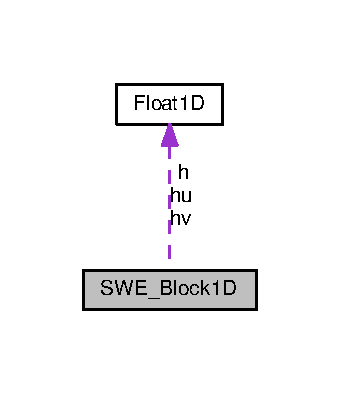
\includegraphics[width=163pt]{structSWE__Block1D__coll__graph}
\end{center}
\end{figure}
\subsection*{Public Member Functions}
\begin{DoxyCompactItemize}
\item 
\hyperlink{structSWE__Block1D_a29516674bf63c42f9fd99995c09f4d55}{S\+W\+E\+\_\+\+Block1D} (const \hyperlink{classFloat1D}{Float1D} \&\+\_\+h, const \hyperlink{classFloat1D}{Float1D} \&\+\_\+hu, const \hyperlink{classFloat1D}{Float1D} \&\+\_\+hv)
\item 
\hyperlink{structSWE__Block1D_a9b23e09458246ba4212a1fbfc52206cc}{S\+W\+E\+\_\+\+Block1D} (float $\ast$\+\_\+h, float $\ast$\+\_\+hu, float $\ast$\+\_\+hv, int \+\_\+size, int \+\_\+stride=1)
\end{DoxyCompactItemize}
\subsection*{Public Attributes}
\begin{DoxyCompactItemize}
\item 
\hyperlink{classFloat1D}{Float1D} \hyperlink{structSWE__Block1D_a7bea1da024ec63e77753fe32880fc5d2}{h}
\item 
\hyperlink{classFloat1D}{Float1D} \hyperlink{structSWE__Block1D_a8662233fe9b86ead9ef2a419103271e5}{hu}
\item 
\hyperlink{classFloat1D}{Float1D} \hyperlink{structSWE__Block1D_aa261d9fcdb400d7da349f41dfa6d5b4f}{hv}
\end{DoxyCompactItemize}


\subsection{Detailed Description}
This file is part S\+WE. 

\hyperlink{structSWE__Block1D}{S\+W\+E\+\_\+\+Block1D} is a simple struct that can represent a single line or row of \hyperlink{classSWE__Block}{S\+W\+E\+\_\+\+Block} unknowns (using the \hyperlink{classFloat1D}{Float1D} proxy class). It is intended to unify the implementation of inflow and periodic boundary conditions, as well as the ghost/copy-\/layer connection between several \hyperlink{classSWE__Block}{S\+W\+E\+\_\+\+Block} grids. 

Definition at line 271 of file S\+W\+E\+\_\+\+Block.\+hh.



\subsection{Constructor \& Destructor Documentation}
\index{S\+W\+E\+\_\+\+Block1D@{S\+W\+E\+\_\+\+Block1D}!S\+W\+E\+\_\+\+Block1D@{S\+W\+E\+\_\+\+Block1D}}
\index{S\+W\+E\+\_\+\+Block1D@{S\+W\+E\+\_\+\+Block1D}!S\+W\+E\+\_\+\+Block1D@{S\+W\+E\+\_\+\+Block1D}}
\subsubsection[{\texorpdfstring{S\+W\+E\+\_\+\+Block1\+D(const Float1\+D \&\+\_\+h, const Float1\+D \&\+\_\+hu, const Float1\+D \&\+\_\+hv)}{SWE_Block1D(const Float1D &_h, const Float1D &_hu, const Float1D &_hv)}}]{\setlength{\rightskip}{0pt plus 5cm}S\+W\+E\+\_\+\+Block1\+D\+::\+S\+W\+E\+\_\+\+Block1D (
\begin{DoxyParamCaption}
\item[{const {\bf Float1D} \&}]{\+\_\+h, }
\item[{const {\bf Float1D} \&}]{\+\_\+hu, }
\item[{const {\bf Float1D} \&}]{\+\_\+hv}
\end{DoxyParamCaption}
)\hspace{0.3cm}{\ttfamily [inline]}}\hypertarget{structSWE__Block1D_a29516674bf63c42f9fd99995c09f4d55}{}\label{structSWE__Block1D_a29516674bf63c42f9fd99995c09f4d55}


Definition at line 272 of file S\+W\+E\+\_\+\+Block.\+hh.

\index{S\+W\+E\+\_\+\+Block1D@{S\+W\+E\+\_\+\+Block1D}!S\+W\+E\+\_\+\+Block1D@{S\+W\+E\+\_\+\+Block1D}}
\index{S\+W\+E\+\_\+\+Block1D@{S\+W\+E\+\_\+\+Block1D}!S\+W\+E\+\_\+\+Block1D@{S\+W\+E\+\_\+\+Block1D}}
\subsubsection[{\texorpdfstring{S\+W\+E\+\_\+\+Block1\+D(float $\ast$\+\_\+h, float $\ast$\+\_\+hu, float $\ast$\+\_\+hv, int \+\_\+size, int \+\_\+stride=1)}{SWE_Block1D(float *_h, float *_hu, float *_hv, int _size, int _stride=1)}}]{\setlength{\rightskip}{0pt plus 5cm}S\+W\+E\+\_\+\+Block1\+D\+::\+S\+W\+E\+\_\+\+Block1D (
\begin{DoxyParamCaption}
\item[{float $\ast$}]{\+\_\+h, }
\item[{float $\ast$}]{\+\_\+hu, }
\item[{float $\ast$}]{\+\_\+hv, }
\item[{int}]{\+\_\+size, }
\item[{int}]{\+\_\+stride = {\ttfamily 1}}
\end{DoxyParamCaption}
)\hspace{0.3cm}{\ttfamily [inline]}}\hypertarget{structSWE__Block1D_a9b23e09458246ba4212a1fbfc52206cc}{}\label{structSWE__Block1D_a9b23e09458246ba4212a1fbfc52206cc}


Definition at line 274 of file S\+W\+E\+\_\+\+Block.\+hh.



\subsection{Member Data Documentation}
\index{S\+W\+E\+\_\+\+Block1D@{S\+W\+E\+\_\+\+Block1D}!h@{h}}
\index{h@{h}!S\+W\+E\+\_\+\+Block1D@{S\+W\+E\+\_\+\+Block1D}}
\subsubsection[{\texorpdfstring{h}{h}}]{\setlength{\rightskip}{0pt plus 5cm}{\bf Float1D} S\+W\+E\+\_\+\+Block1\+D\+::h}\hypertarget{structSWE__Block1D_a7bea1da024ec63e77753fe32880fc5d2}{}\label{structSWE__Block1D_a7bea1da024ec63e77753fe32880fc5d2}


Definition at line 275 of file S\+W\+E\+\_\+\+Block.\+hh.

\index{S\+W\+E\+\_\+\+Block1D@{S\+W\+E\+\_\+\+Block1D}!hu@{hu}}
\index{hu@{hu}!S\+W\+E\+\_\+\+Block1D@{S\+W\+E\+\_\+\+Block1D}}
\subsubsection[{\texorpdfstring{hu}{hu}}]{\setlength{\rightskip}{0pt plus 5cm}{\bf Float1D} S\+W\+E\+\_\+\+Block1\+D\+::hu}\hypertarget{structSWE__Block1D_a8662233fe9b86ead9ef2a419103271e5}{}\label{structSWE__Block1D_a8662233fe9b86ead9ef2a419103271e5}


Definition at line 278 of file S\+W\+E\+\_\+\+Block.\+hh.

\index{S\+W\+E\+\_\+\+Block1D@{S\+W\+E\+\_\+\+Block1D}!hv@{hv}}
\index{hv@{hv}!S\+W\+E\+\_\+\+Block1D@{S\+W\+E\+\_\+\+Block1D}}
\subsubsection[{\texorpdfstring{hv}{hv}}]{\setlength{\rightskip}{0pt plus 5cm}{\bf Float1D} S\+W\+E\+\_\+\+Block1\+D\+::hv}\hypertarget{structSWE__Block1D_aa261d9fcdb400d7da349f41dfa6d5b4f}{}\label{structSWE__Block1D_aa261d9fcdb400d7da349f41dfa6d5b4f}


Definition at line 279 of file S\+W\+E\+\_\+\+Block.\+hh.



The documentation for this class was generated from the following file\+:\begin{DoxyCompactItemize}
\item 
app/src/main/cpp/blocks/\hyperlink{SWE__Block_8hh}{S\+W\+E\+\_\+\+Block.\+hh}\end{DoxyCompactItemize}

\hypertarget{classSWE__FlatScenario}{}\section{S\+W\+E\+\_\+\+Flat\+Scenario Class Reference}
\label{classSWE__FlatScenario}\index{S\+W\+E\+\_\+\+Flat\+Scenario@{S\+W\+E\+\_\+\+Flat\+Scenario}}


scenario is a test environment that simulates a flat water-\/surface  




{\ttfamily \#include $<$S\+W\+E\+\_\+simple\+\_\+scenarios.\+hh$>$}



Inheritance diagram for S\+W\+E\+\_\+\+Flat\+Scenario\+:\nopagebreak
\begin{figure}[H]
\begin{center}
\leavevmode
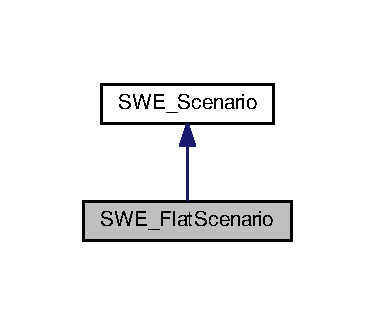
\includegraphics[width=180pt]{classSWE__FlatScenario__inherit__graph}
\end{center}
\end{figure}


Collaboration diagram for S\+W\+E\+\_\+\+Flat\+Scenario\+:\nopagebreak
\begin{figure}[H]
\begin{center}
\leavevmode
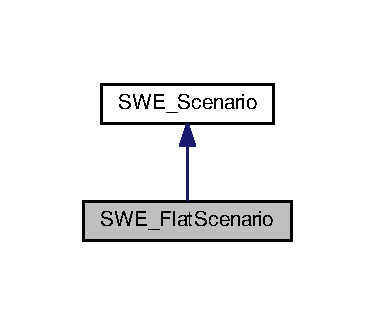
\includegraphics[width=180pt]{classSWE__FlatScenario__coll__graph}
\end{center}
\end{figure}
\subsection*{Public Member Functions}
\begin{DoxyCompactItemize}
\item 
float \hyperlink{classSWE__FlatScenario_a0e0bcfaa2ccacf0716df4e818e47ea75}{get\+Bathymetry} (float x, float y)
\item 
float \hyperlink{classSWE__FlatScenario_a8391be8368aa74a4439977328f42f1db}{get\+Water\+Height} (float x, float y)
\item 
virtual float \hyperlink{classSWE__FlatScenario_a639126b73114a940a4e1d3cfb1bd2050}{end\+Simulation} ()
\item 
virtual \hyperlink{scenarios_2SWE__Scenario_8hh_af75d5dd7322fa39ed0af4e7839e600f8}{Boundary\+Type} \hyperlink{classSWE__FlatScenario_ac290c261f5a73b4a42defdc71a70ec0e}{get\+Boundary\+Type} (\hyperlink{scenarios_2SWE__Scenario_8hh_aa5e01e3f7df312f7b9b0d02521141fcc}{Boundary\+Edge} edge)
\item 
float \hyperlink{classSWE__FlatScenario_a046d055ee2e6f20a0509801f5fbe7d58}{get\+Boundary\+Pos} (\hyperlink{scenarios_2SWE__Scenario_8hh_aa5e01e3f7df312f7b9b0d02521141fcc}{Boundary\+Edge} i\+\_\+edge)
\end{DoxyCompactItemize}


\subsection{Detailed Description}
scenario is a test environment that simulates a flat water-\/surface 

Scenario \char`\"{}\+Radial Dam Break\char`\"{}\+: elevated water in the center of the domain 

Definition at line 41 of file S\+W\+E\+\_\+simple\+\_\+scenarios.\+hh.



\subsection{Member Function Documentation}
\index{S\+W\+E\+\_\+\+Flat\+Scenario@{S\+W\+E\+\_\+\+Flat\+Scenario}!end\+Simulation@{end\+Simulation}}
\index{end\+Simulation@{end\+Simulation}!S\+W\+E\+\_\+\+Flat\+Scenario@{S\+W\+E\+\_\+\+Flat\+Scenario}}
\subsubsection[{\texorpdfstring{end\+Simulation()}{endSimulation()}}]{\setlength{\rightskip}{0pt plus 5cm}virtual float S\+W\+E\+\_\+\+Flat\+Scenario\+::end\+Simulation (
\begin{DoxyParamCaption}
{}
\end{DoxyParamCaption}
)\hspace{0.3cm}{\ttfamily [inline]}, {\ttfamily [virtual]}}\hypertarget{classSWE__FlatScenario_a639126b73114a940a4e1d3cfb1bd2050}{}\label{classSWE__FlatScenario_a639126b73114a940a4e1d3cfb1bd2050}


Reimplemented from \hyperlink{classSWE__Scenario_ae7ed72f584069e9885c33c4ca83f3ff5}{S\+W\+E\+\_\+\+Scenario}.



Definition at line 54 of file S\+W\+E\+\_\+simple\+\_\+scenarios.\+hh.

\index{S\+W\+E\+\_\+\+Flat\+Scenario@{S\+W\+E\+\_\+\+Flat\+Scenario}!get\+Bathymetry@{get\+Bathymetry}}
\index{get\+Bathymetry@{get\+Bathymetry}!S\+W\+E\+\_\+\+Flat\+Scenario@{S\+W\+E\+\_\+\+Flat\+Scenario}}
\subsubsection[{\texorpdfstring{get\+Bathymetry(float x, float y)}{getBathymetry(float x, float y)}}]{\setlength{\rightskip}{0pt plus 5cm}float S\+W\+E\+\_\+\+Flat\+Scenario\+::get\+Bathymetry (
\begin{DoxyParamCaption}
\item[{float}]{x, }
\item[{float}]{y}
\end{DoxyParamCaption}
)\hspace{0.3cm}{\ttfamily [inline]}, {\ttfamily [virtual]}}\hypertarget{classSWE__FlatScenario_a0e0bcfaa2ccacf0716df4e818e47ea75}{}\label{classSWE__FlatScenario_a0e0bcfaa2ccacf0716df4e818e47ea75}


Reimplemented from \hyperlink{classSWE__Scenario_afe09a1ba63304800651f25873570a348}{S\+W\+E\+\_\+\+Scenario}.



Definition at line 45 of file S\+W\+E\+\_\+simple\+\_\+scenarios.\+hh.

\index{S\+W\+E\+\_\+\+Flat\+Scenario@{S\+W\+E\+\_\+\+Flat\+Scenario}!get\+Boundary\+Pos@{get\+Boundary\+Pos}}
\index{get\+Boundary\+Pos@{get\+Boundary\+Pos}!S\+W\+E\+\_\+\+Flat\+Scenario@{S\+W\+E\+\_\+\+Flat\+Scenario}}
\subsubsection[{\texorpdfstring{get\+Boundary\+Pos(\+Boundary\+Edge i\+\_\+edge)}{getBoundaryPos(BoundaryEdge i_edge)}}]{\setlength{\rightskip}{0pt plus 5cm}float S\+W\+E\+\_\+\+Flat\+Scenario\+::get\+Boundary\+Pos (
\begin{DoxyParamCaption}
\item[{{\bf Boundary\+Edge}}]{i\+\_\+edge}
\end{DoxyParamCaption}
)\hspace{0.3cm}{\ttfamily [inline]}, {\ttfamily [virtual]}}\hypertarget{classSWE__FlatScenario_a046d055ee2e6f20a0509801f5fbe7d58}{}\label{classSWE__FlatScenario_a046d055ee2e6f20a0509801f5fbe7d58}
Get the boundary positions


\begin{DoxyParams}{Parameters}
{\em i\+\_\+edge} & which edge \\
\hline
\end{DoxyParams}
\begin{DoxyReturn}{Returns}
value in the corresponding dimension 
\end{DoxyReturn}


Reimplemented from \hyperlink{classSWE__Scenario_a1b01e953c2079b64f527c9bc5a0c86d7}{S\+W\+E\+\_\+\+Scenario}.



Definition at line 63 of file S\+W\+E\+\_\+simple\+\_\+scenarios.\+hh.

\index{S\+W\+E\+\_\+\+Flat\+Scenario@{S\+W\+E\+\_\+\+Flat\+Scenario}!get\+Boundary\+Type@{get\+Boundary\+Type}}
\index{get\+Boundary\+Type@{get\+Boundary\+Type}!S\+W\+E\+\_\+\+Flat\+Scenario@{S\+W\+E\+\_\+\+Flat\+Scenario}}
\subsubsection[{\texorpdfstring{get\+Boundary\+Type(\+Boundary\+Edge edge)}{getBoundaryType(BoundaryEdge edge)}}]{\setlength{\rightskip}{0pt plus 5cm}virtual {\bf Boundary\+Type} S\+W\+E\+\_\+\+Flat\+Scenario\+::get\+Boundary\+Type (
\begin{DoxyParamCaption}
\item[{{\bf Boundary\+Edge}}]{edge}
\end{DoxyParamCaption}
)\hspace{0.3cm}{\ttfamily [inline]}, {\ttfamily [virtual]}}\hypertarget{classSWE__FlatScenario_ac290c261f5a73b4a42defdc71a70ec0e}{}\label{classSWE__FlatScenario_ac290c261f5a73b4a42defdc71a70ec0e}


Reimplemented from \hyperlink{classSWE__Scenario_ab8fe7ce15d7758fb0c4e0e3887b34a5d}{S\+W\+E\+\_\+\+Scenario}.



Definition at line 56 of file S\+W\+E\+\_\+simple\+\_\+scenarios.\+hh.

\index{S\+W\+E\+\_\+\+Flat\+Scenario@{S\+W\+E\+\_\+\+Flat\+Scenario}!get\+Water\+Height@{get\+Water\+Height}}
\index{get\+Water\+Height@{get\+Water\+Height}!S\+W\+E\+\_\+\+Flat\+Scenario@{S\+W\+E\+\_\+\+Flat\+Scenario}}
\subsubsection[{\texorpdfstring{get\+Water\+Height(float x, float y)}{getWaterHeight(float x, float y)}}]{\setlength{\rightskip}{0pt plus 5cm}float S\+W\+E\+\_\+\+Flat\+Scenario\+::get\+Water\+Height (
\begin{DoxyParamCaption}
\item[{float}]{x, }
\item[{float}]{y}
\end{DoxyParamCaption}
)\hspace{0.3cm}{\ttfamily [inline]}, {\ttfamily [virtual]}}\hypertarget{classSWE__FlatScenario_a8391be8368aa74a4439977328f42f1db}{}\label{classSWE__FlatScenario_a8391be8368aa74a4439977328f42f1db}


Reimplemented from \hyperlink{classSWE__Scenario_ade6f356d60b1402c034611266462b88b}{S\+W\+E\+\_\+\+Scenario}.



Definition at line 49 of file S\+W\+E\+\_\+simple\+\_\+scenarios.\+hh.



The documentation for this class was generated from the following file\+:\begin{DoxyCompactItemize}
\item 
app/src/main/cpp/scenarios/\hyperlink{SWE__simple__scenarios_8hh}{S\+W\+E\+\_\+simple\+\_\+scenarios.\+hh}\end{DoxyCompactItemize}

\hypertarget{classSWE__Scenario}{}\section{S\+W\+E\+\_\+\+Scenario Class Reference}
\label{classSWE__Scenario}\index{S\+W\+E\+\_\+\+Scenario@{S\+W\+E\+\_\+\+Scenario}}


This class sets the standart layout for all simulateable scenarios.  




{\ttfamily \#include $<$S\+W\+E\+\_\+\+Scenario.\+hh$>$}



Inheritance diagram for S\+W\+E\+\_\+\+Scenario\+:\nopagebreak
\begin{figure}[H]
\begin{center}
\leavevmode
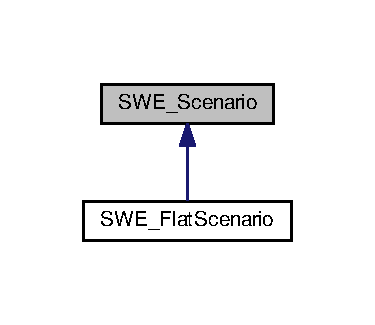
\includegraphics[width=238pt]{classSWE__Scenario__inherit__graph}
\end{center}
\end{figure}
\subsection*{Public Member Functions}
\begin{DoxyCompactItemize}
\item 
virtual float \hyperlink{classSWE__Scenario_ade6f356d60b1402c034611266462b88b}{get\+Water\+Height} (float x, float y)
\item 
virtual float \hyperlink{classSWE__Scenario_ab1d5e360c861df3c8c0ccd919bd7f495}{get\+Veloc\+\_\+u} (float x, float y)
\item 
virtual float \hyperlink{classSWE__Scenario_afeaf75872a1678ea64e6f7accd1e49c6}{get\+Veloc\+\_\+v} (float x, float y)
\item 
virtual float \hyperlink{classSWE__Scenario_afe09a1ba63304800651f25873570a348}{get\+Bathymetry} (float x, float y)
\item 
virtual float \hyperlink{classSWE__Scenario_a9de0f0f9fcc34dfe00c522b10c343d91}{water\+Height\+At\+Rest} ()
\item 
virtual float \hyperlink{classSWE__Scenario_ae7ed72f584069e9885c33c4ca83f3ff5}{end\+Simulation} ()
\item 
virtual \hyperlink{scenarios_2SWE__Scenario_8hh_af75d5dd7322fa39ed0af4e7839e600f8}{Boundary\+Type} \hyperlink{classSWE__Scenario_ab8fe7ce15d7758fb0c4e0e3887b34a5d}{get\+Boundary\+Type} (\hyperlink{scenarios_2SWE__Scenario_8hh_aa5e01e3f7df312f7b9b0d02521141fcc}{Boundary\+Edge} edge)
\item 
virtual float \hyperlink{classSWE__Scenario_a1b01e953c2079b64f527c9bc5a0c86d7}{get\+Boundary\+Pos} (\hyperlink{scenarios_2SWE__Scenario_8hh_aa5e01e3f7df312f7b9b0d02521141fcc}{Boundary\+Edge} edge)
\item 
virtual \hyperlink{classSWE__Scenario_a5e20e1061abfa36d814e0650a12a2e69}{$\sim$\+S\+W\+E\+\_\+\+Scenario} ()
\item 
virtual float \hyperlink{classSWE__Scenario_ade6f356d60b1402c034611266462b88b}{get\+Water\+Height} (float x, float y)
\item 
virtual float \hyperlink{classSWE__Scenario_ab1d5e360c861df3c8c0ccd919bd7f495}{get\+Veloc\+\_\+u} (float x, float y)
\item 
virtual float \hyperlink{classSWE__Scenario_afeaf75872a1678ea64e6f7accd1e49c6}{get\+Veloc\+\_\+v} (float x, float y)
\item 
virtual float \hyperlink{classSWE__Scenario_afe09a1ba63304800651f25873570a348}{get\+Bathymetry} (float x, float y)
\item 
virtual float \hyperlink{classSWE__Scenario_a9de0f0f9fcc34dfe00c522b10c343d91}{water\+Height\+At\+Rest} ()
\item 
virtual float \hyperlink{classSWE__Scenario_ae7ed72f584069e9885c33c4ca83f3ff5}{end\+Simulation} ()
\item 
virtual \hyperlink{scenarios_2SWE__Scenario_8hh_af75d5dd7322fa39ed0af4e7839e600f8}{Boundary\+Type} \hyperlink{classSWE__Scenario_ab8fe7ce15d7758fb0c4e0e3887b34a5d}{get\+Boundary\+Type} (\hyperlink{scenarios_2SWE__Scenario_8hh_aa5e01e3f7df312f7b9b0d02521141fcc}{Boundary\+Edge} edge)
\item 
virtual float \hyperlink{classSWE__Scenario_a1b01e953c2079b64f527c9bc5a0c86d7}{get\+Boundary\+Pos} (\hyperlink{scenarios_2SWE__Scenario_8hh_aa5e01e3f7df312f7b9b0d02521141fcc}{Boundary\+Edge} edge)
\item 
virtual \hyperlink{classSWE__Scenario_a5e20e1061abfa36d814e0650a12a2e69}{$\sim$\+S\+W\+E\+\_\+\+Scenario} ()
\end{DoxyCompactItemize}


\subsection{Detailed Description}
This class sets the standart layout for all simulateable scenarios. 

\hyperlink{classSWE__Scenario}{S\+W\+E\+\_\+\+Scenario} defines an interface to initialise the unknowns of a shallow water simulation -\/ i.\+e. to initialise water height, velocities, and bathymatry according to certain scenarios. \hyperlink{classSWE__Scenario}{S\+W\+E\+\_\+\+Scenario} can act as stand-\/alone scenario class, providing a very basic scenario (all functions are constant); however, the idea is to provide derived classes that implement the \hyperlink{classSWE__Scenario}{S\+W\+E\+\_\+\+Scenario} interface for more interesting scenarios. 

Definition at line 55 of file S\+W\+E\+\_\+\+Scenario.\+hh.



\subsection{Constructor \& Destructor Documentation}
\index{S\+W\+E\+\_\+\+Scenario@{S\+W\+E\+\_\+\+Scenario}!````~S\+W\+E\+\_\+\+Scenario@{$\sim$\+S\+W\+E\+\_\+\+Scenario}}
\index{````~S\+W\+E\+\_\+\+Scenario@{$\sim$\+S\+W\+E\+\_\+\+Scenario}!S\+W\+E\+\_\+\+Scenario@{S\+W\+E\+\_\+\+Scenario}}
\subsubsection[{\texorpdfstring{$\sim$\+S\+W\+E\+\_\+\+Scenario()}{~SWE_Scenario()}}]{\setlength{\rightskip}{0pt plus 5cm}virtual S\+W\+E\+\_\+\+Scenario\+::$\sim$\+S\+W\+E\+\_\+\+Scenario (
\begin{DoxyParamCaption}
{}
\end{DoxyParamCaption}
)\hspace{0.3cm}{\ttfamily [inline]}, {\ttfamily [virtual]}}\hypertarget{classSWE__Scenario_a5e20e1061abfa36d814e0650a12a2e69}{}\label{classSWE__Scenario_a5e20e1061abfa36d814e0650a12a2e69}


Definition at line 76 of file S\+W\+E\+\_\+\+Scenario.\+hh.

\index{S\+W\+E\+\_\+\+Scenario@{S\+W\+E\+\_\+\+Scenario}!````~S\+W\+E\+\_\+\+Scenario@{$\sim$\+S\+W\+E\+\_\+\+Scenario}}
\index{````~S\+W\+E\+\_\+\+Scenario@{$\sim$\+S\+W\+E\+\_\+\+Scenario}!S\+W\+E\+\_\+\+Scenario@{S\+W\+E\+\_\+\+Scenario}}
\subsubsection[{\texorpdfstring{$\sim$\+S\+W\+E\+\_\+\+Scenario()}{~SWE_Scenario()}}]{\setlength{\rightskip}{0pt plus 5cm}virtual S\+W\+E\+\_\+\+Scenario\+::$\sim$\+S\+W\+E\+\_\+\+Scenario (
\begin{DoxyParamCaption}
{}
\end{DoxyParamCaption}
)\hspace{0.3cm}{\ttfamily [inline]}, {\ttfamily [virtual]}}\hypertarget{classSWE__Scenario_a5e20e1061abfa36d814e0650a12a2e69}{}\label{classSWE__Scenario_a5e20e1061abfa36d814e0650a12a2e69}


Definition at line 75 of file S\+W\+E\+\_\+\+Scenario.\+hh.



\subsection{Member Function Documentation}
\index{S\+W\+E\+\_\+\+Scenario@{S\+W\+E\+\_\+\+Scenario}!end\+Simulation@{end\+Simulation}}
\index{end\+Simulation@{end\+Simulation}!S\+W\+E\+\_\+\+Scenario@{S\+W\+E\+\_\+\+Scenario}}
\subsubsection[{\texorpdfstring{end\+Simulation()}{endSimulation()}}]{\setlength{\rightskip}{0pt plus 5cm}virtual float S\+W\+E\+\_\+\+Scenario\+::end\+Simulation (
\begin{DoxyParamCaption}
{}
\end{DoxyParamCaption}
)\hspace{0.3cm}{\ttfamily [inline]}, {\ttfamily [virtual]}}\hypertarget{classSWE__Scenario_ae7ed72f584069e9885c33c4ca83f3ff5}{}\label{classSWE__Scenario_ae7ed72f584069e9885c33c4ca83f3ff5}


Reimplemented in \hyperlink{classSWE__RadialDamBreakScenario_a5e118a3d34aace3175745965d5d9c567}{S\+W\+E\+\_\+\+Radial\+Dam\+Break\+Scenario}.



Definition at line 65 of file S\+W\+E\+\_\+\+Scenario.\+hh.

\index{S\+W\+E\+\_\+\+Scenario@{S\+W\+E\+\_\+\+Scenario}!end\+Simulation@{end\+Simulation}}
\index{end\+Simulation@{end\+Simulation}!S\+W\+E\+\_\+\+Scenario@{S\+W\+E\+\_\+\+Scenario}}
\subsubsection[{\texorpdfstring{end\+Simulation()}{endSimulation()}}]{\setlength{\rightskip}{0pt plus 5cm}virtual float S\+W\+E\+\_\+\+Scenario\+::end\+Simulation (
\begin{DoxyParamCaption}
{}
\end{DoxyParamCaption}
)\hspace{0.3cm}{\ttfamily [inline]}, {\ttfamily [virtual]}}\hypertarget{classSWE__Scenario_ae7ed72f584069e9885c33c4ca83f3ff5}{}\label{classSWE__Scenario_ae7ed72f584069e9885c33c4ca83f3ff5}


Reimplemented in \hyperlink{classSWE__RadialDamBreakScenario_a5e118a3d34aace3175745965d5d9c567}{S\+W\+E\+\_\+\+Radial\+Dam\+Break\+Scenario}.



Definition at line 66 of file S\+W\+E\+\_\+\+Scenario.\+hh.

\index{S\+W\+E\+\_\+\+Scenario@{S\+W\+E\+\_\+\+Scenario}!get\+Bathymetry@{get\+Bathymetry}}
\index{get\+Bathymetry@{get\+Bathymetry}!S\+W\+E\+\_\+\+Scenario@{S\+W\+E\+\_\+\+Scenario}}
\subsubsection[{\texorpdfstring{get\+Bathymetry(float x, float y)}{getBathymetry(float x, float y)}}]{\setlength{\rightskip}{0pt plus 5cm}virtual float S\+W\+E\+\_\+\+Scenario\+::get\+Bathymetry (
\begin{DoxyParamCaption}
\item[{float}]{x, }
\item[{float}]{y}
\end{DoxyParamCaption}
)\hspace{0.3cm}{\ttfamily [inline]}, {\ttfamily [virtual]}}\hypertarget{classSWE__Scenario_afe09a1ba63304800651f25873570a348}{}\label{classSWE__Scenario_afe09a1ba63304800651f25873570a348}


Reimplemented in \hyperlink{classSWE__RadialDamBreakScenario_ab54c88d18ff3a577a3e33f1659d97b50}{S\+W\+E\+\_\+\+Radial\+Dam\+Break\+Scenario}.



Definition at line 61 of file S\+W\+E\+\_\+\+Scenario.\+hh.

\index{S\+W\+E\+\_\+\+Scenario@{S\+W\+E\+\_\+\+Scenario}!get\+Bathymetry@{get\+Bathymetry}}
\index{get\+Bathymetry@{get\+Bathymetry}!S\+W\+E\+\_\+\+Scenario@{S\+W\+E\+\_\+\+Scenario}}
\subsubsection[{\texorpdfstring{get\+Bathymetry(float x, float y)}{getBathymetry(float x, float y)}}]{\setlength{\rightskip}{0pt plus 5cm}virtual float S\+W\+E\+\_\+\+Scenario\+::get\+Bathymetry (
\begin{DoxyParamCaption}
\item[{float}]{x, }
\item[{float}]{y}
\end{DoxyParamCaption}
)\hspace{0.3cm}{\ttfamily [inline]}, {\ttfamily [virtual]}}\hypertarget{classSWE__Scenario_afe09a1ba63304800651f25873570a348}{}\label{classSWE__Scenario_afe09a1ba63304800651f25873570a348}


Reimplemented in \hyperlink{classSWE__RadialDamBreakScenario_ab54c88d18ff3a577a3e33f1659d97b50}{S\+W\+E\+\_\+\+Radial\+Dam\+Break\+Scenario}.



Definition at line 62 of file S\+W\+E\+\_\+\+Scenario.\+hh.

\index{S\+W\+E\+\_\+\+Scenario@{S\+W\+E\+\_\+\+Scenario}!get\+Boundary\+Pos@{get\+Boundary\+Pos}}
\index{get\+Boundary\+Pos@{get\+Boundary\+Pos}!S\+W\+E\+\_\+\+Scenario@{S\+W\+E\+\_\+\+Scenario}}
\subsubsection[{\texorpdfstring{get\+Boundary\+Pos(\+Boundary\+Edge edge)}{getBoundaryPos(BoundaryEdge edge)}}]{\setlength{\rightskip}{0pt plus 5cm}virtual float S\+W\+E\+\_\+\+Scenario\+::get\+Boundary\+Pos (
\begin{DoxyParamCaption}
\item[{{\bf Boundary\+Edge}}]{edge}
\end{DoxyParamCaption}
)\hspace{0.3cm}{\ttfamily [inline]}, {\ttfamily [virtual]}}\hypertarget{classSWE__Scenario_a1b01e953c2079b64f527c9bc5a0c86d7}{}\label{classSWE__Scenario_a1b01e953c2079b64f527c9bc5a0c86d7}


Reimplemented in \hyperlink{classSWE__RadialDamBreakScenario_ac5392df630c8164560df5cb902df385a}{S\+W\+E\+\_\+\+Radial\+Dam\+Break\+Scenario}.



Definition at line 68 of file S\+W\+E\+\_\+\+Scenario.\+hh.

\index{S\+W\+E\+\_\+\+Scenario@{S\+W\+E\+\_\+\+Scenario}!get\+Boundary\+Pos@{get\+Boundary\+Pos}}
\index{get\+Boundary\+Pos@{get\+Boundary\+Pos}!S\+W\+E\+\_\+\+Scenario@{S\+W\+E\+\_\+\+Scenario}}
\subsubsection[{\texorpdfstring{get\+Boundary\+Pos(\+Boundary\+Edge edge)}{getBoundaryPos(BoundaryEdge edge)}}]{\setlength{\rightskip}{0pt plus 5cm}virtual float S\+W\+E\+\_\+\+Scenario\+::get\+Boundary\+Pos (
\begin{DoxyParamCaption}
\item[{{\bf Boundary\+Edge}}]{edge}
\end{DoxyParamCaption}
)\hspace{0.3cm}{\ttfamily [inline]}, {\ttfamily [virtual]}}\hypertarget{classSWE__Scenario_a1b01e953c2079b64f527c9bc5a0c86d7}{}\label{classSWE__Scenario_a1b01e953c2079b64f527c9bc5a0c86d7}


Reimplemented in \hyperlink{classSWE__RadialDamBreakScenario_ac5392df630c8164560df5cb902df385a}{S\+W\+E\+\_\+\+Radial\+Dam\+Break\+Scenario}.



Definition at line 69 of file S\+W\+E\+\_\+\+Scenario.\+hh.

\index{S\+W\+E\+\_\+\+Scenario@{S\+W\+E\+\_\+\+Scenario}!get\+Boundary\+Type@{get\+Boundary\+Type}}
\index{get\+Boundary\+Type@{get\+Boundary\+Type}!S\+W\+E\+\_\+\+Scenario@{S\+W\+E\+\_\+\+Scenario}}
\subsubsection[{\texorpdfstring{get\+Boundary\+Type(\+Boundary\+Edge edge)}{getBoundaryType(BoundaryEdge edge)}}]{\setlength{\rightskip}{0pt plus 5cm}virtual {\bf Boundary\+Type} S\+W\+E\+\_\+\+Scenario\+::get\+Boundary\+Type (
\begin{DoxyParamCaption}
\item[{{\bf Boundary\+Edge}}]{edge}
\end{DoxyParamCaption}
)\hspace{0.3cm}{\ttfamily [inline]}, {\ttfamily [virtual]}}\hypertarget{classSWE__Scenario_ab8fe7ce15d7758fb0c4e0e3887b34a5d}{}\label{classSWE__Scenario_ab8fe7ce15d7758fb0c4e0e3887b34a5d}


Reimplemented in \hyperlink{classSWE__RadialDamBreakScenario_a40a7ddfd7d85631eeb708232c9f7f20d}{S\+W\+E\+\_\+\+Radial\+Dam\+Break\+Scenario}.



Definition at line 67 of file S\+W\+E\+\_\+\+Scenario.\+hh.

\index{S\+W\+E\+\_\+\+Scenario@{S\+W\+E\+\_\+\+Scenario}!get\+Boundary\+Type@{get\+Boundary\+Type}}
\index{get\+Boundary\+Type@{get\+Boundary\+Type}!S\+W\+E\+\_\+\+Scenario@{S\+W\+E\+\_\+\+Scenario}}
\subsubsection[{\texorpdfstring{get\+Boundary\+Type(\+Boundary\+Edge edge)}{getBoundaryType(BoundaryEdge edge)}}]{\setlength{\rightskip}{0pt plus 5cm}virtual {\bf Boundary\+Type} S\+W\+E\+\_\+\+Scenario\+::get\+Boundary\+Type (
\begin{DoxyParamCaption}
\item[{{\bf Boundary\+Edge}}]{edge}
\end{DoxyParamCaption}
)\hspace{0.3cm}{\ttfamily [inline]}, {\ttfamily [virtual]}}\hypertarget{classSWE__Scenario_ab8fe7ce15d7758fb0c4e0e3887b34a5d}{}\label{classSWE__Scenario_ab8fe7ce15d7758fb0c4e0e3887b34a5d}


Reimplemented in \hyperlink{classSWE__RadialDamBreakScenario_a40a7ddfd7d85631eeb708232c9f7f20d}{S\+W\+E\+\_\+\+Radial\+Dam\+Break\+Scenario}.



Definition at line 68 of file S\+W\+E\+\_\+\+Scenario.\+hh.

\index{S\+W\+E\+\_\+\+Scenario@{S\+W\+E\+\_\+\+Scenario}!get\+Veloc\+\_\+u@{get\+Veloc\+\_\+u}}
\index{get\+Veloc\+\_\+u@{get\+Veloc\+\_\+u}!S\+W\+E\+\_\+\+Scenario@{S\+W\+E\+\_\+\+Scenario}}
\subsubsection[{\texorpdfstring{get\+Veloc\+\_\+u(float x, float y)}{getVeloc_u(float x, float y)}}]{\setlength{\rightskip}{0pt plus 5cm}virtual float S\+W\+E\+\_\+\+Scenario\+::get\+Veloc\+\_\+u (
\begin{DoxyParamCaption}
\item[{float}]{x, }
\item[{float}]{y}
\end{DoxyParamCaption}
)\hspace{0.3cm}{\ttfamily [inline]}, {\ttfamily [virtual]}}\hypertarget{classSWE__Scenario_ab1d5e360c861df3c8c0ccd919bd7f495}{}\label{classSWE__Scenario_ab1d5e360c861df3c8c0ccd919bd7f495}


Definition at line 59 of file S\+W\+E\+\_\+\+Scenario.\+hh.

\index{S\+W\+E\+\_\+\+Scenario@{S\+W\+E\+\_\+\+Scenario}!get\+Veloc\+\_\+u@{get\+Veloc\+\_\+u}}
\index{get\+Veloc\+\_\+u@{get\+Veloc\+\_\+u}!S\+W\+E\+\_\+\+Scenario@{S\+W\+E\+\_\+\+Scenario}}
\subsubsection[{\texorpdfstring{get\+Veloc\+\_\+u(float x, float y)}{getVeloc_u(float x, float y)}}]{\setlength{\rightskip}{0pt plus 5cm}virtual float S\+W\+E\+\_\+\+Scenario\+::get\+Veloc\+\_\+u (
\begin{DoxyParamCaption}
\item[{float}]{x, }
\item[{float}]{y}
\end{DoxyParamCaption}
)\hspace{0.3cm}{\ttfamily [inline]}, {\ttfamily [virtual]}}\hypertarget{classSWE__Scenario_ab1d5e360c861df3c8c0ccd919bd7f495}{}\label{classSWE__Scenario_ab1d5e360c861df3c8c0ccd919bd7f495}


Definition at line 60 of file S\+W\+E\+\_\+\+Scenario.\+hh.

\index{S\+W\+E\+\_\+\+Scenario@{S\+W\+E\+\_\+\+Scenario}!get\+Veloc\+\_\+v@{get\+Veloc\+\_\+v}}
\index{get\+Veloc\+\_\+v@{get\+Veloc\+\_\+v}!S\+W\+E\+\_\+\+Scenario@{S\+W\+E\+\_\+\+Scenario}}
\subsubsection[{\texorpdfstring{get\+Veloc\+\_\+v(float x, float y)}{getVeloc_v(float x, float y)}}]{\setlength{\rightskip}{0pt plus 5cm}virtual float S\+W\+E\+\_\+\+Scenario\+::get\+Veloc\+\_\+v (
\begin{DoxyParamCaption}
\item[{float}]{x, }
\item[{float}]{y}
\end{DoxyParamCaption}
)\hspace{0.3cm}{\ttfamily [inline]}, {\ttfamily [virtual]}}\hypertarget{classSWE__Scenario_afeaf75872a1678ea64e6f7accd1e49c6}{}\label{classSWE__Scenario_afeaf75872a1678ea64e6f7accd1e49c6}


Definition at line 60 of file S\+W\+E\+\_\+\+Scenario.\+hh.

\index{S\+W\+E\+\_\+\+Scenario@{S\+W\+E\+\_\+\+Scenario}!get\+Veloc\+\_\+v@{get\+Veloc\+\_\+v}}
\index{get\+Veloc\+\_\+v@{get\+Veloc\+\_\+v}!S\+W\+E\+\_\+\+Scenario@{S\+W\+E\+\_\+\+Scenario}}
\subsubsection[{\texorpdfstring{get\+Veloc\+\_\+v(float x, float y)}{getVeloc_v(float x, float y)}}]{\setlength{\rightskip}{0pt plus 5cm}virtual float S\+W\+E\+\_\+\+Scenario\+::get\+Veloc\+\_\+v (
\begin{DoxyParamCaption}
\item[{float}]{x, }
\item[{float}]{y}
\end{DoxyParamCaption}
)\hspace{0.3cm}{\ttfamily [inline]}, {\ttfamily [virtual]}}\hypertarget{classSWE__Scenario_afeaf75872a1678ea64e6f7accd1e49c6}{}\label{classSWE__Scenario_afeaf75872a1678ea64e6f7accd1e49c6}


Definition at line 61 of file S\+W\+E\+\_\+\+Scenario.\+hh.

\index{S\+W\+E\+\_\+\+Scenario@{S\+W\+E\+\_\+\+Scenario}!get\+Water\+Height@{get\+Water\+Height}}
\index{get\+Water\+Height@{get\+Water\+Height}!S\+W\+E\+\_\+\+Scenario@{S\+W\+E\+\_\+\+Scenario}}
\subsubsection[{\texorpdfstring{get\+Water\+Height(float x, float y)}{getWaterHeight(float x, float y)}}]{\setlength{\rightskip}{0pt plus 5cm}virtual float S\+W\+E\+\_\+\+Scenario\+::get\+Water\+Height (
\begin{DoxyParamCaption}
\item[{float}]{x, }
\item[{float}]{y}
\end{DoxyParamCaption}
)\hspace{0.3cm}{\ttfamily [inline]}, {\ttfamily [virtual]}}\hypertarget{classSWE__Scenario_ade6f356d60b1402c034611266462b88b}{}\label{classSWE__Scenario_ade6f356d60b1402c034611266462b88b}


Reimplemented in \hyperlink{classSWE__RadialDamBreakScenario_a0fb0917dd1e47f9580bd94ba5816795c}{S\+W\+E\+\_\+\+Radial\+Dam\+Break\+Scenario}.



Definition at line 58 of file S\+W\+E\+\_\+\+Scenario.\+hh.

\index{S\+W\+E\+\_\+\+Scenario@{S\+W\+E\+\_\+\+Scenario}!get\+Water\+Height@{get\+Water\+Height}}
\index{get\+Water\+Height@{get\+Water\+Height}!S\+W\+E\+\_\+\+Scenario@{S\+W\+E\+\_\+\+Scenario}}
\subsubsection[{\texorpdfstring{get\+Water\+Height(float x, float y)}{getWaterHeight(float x, float y)}}]{\setlength{\rightskip}{0pt plus 5cm}virtual float S\+W\+E\+\_\+\+Scenario\+::get\+Water\+Height (
\begin{DoxyParamCaption}
\item[{float}]{x, }
\item[{float}]{y}
\end{DoxyParamCaption}
)\hspace{0.3cm}{\ttfamily [inline]}, {\ttfamily [virtual]}}\hypertarget{classSWE__Scenario_ade6f356d60b1402c034611266462b88b}{}\label{classSWE__Scenario_ade6f356d60b1402c034611266462b88b}


Reimplemented in \hyperlink{classSWE__RadialDamBreakScenario_a0fb0917dd1e47f9580bd94ba5816795c}{S\+W\+E\+\_\+\+Radial\+Dam\+Break\+Scenario}.



Definition at line 59 of file S\+W\+E\+\_\+\+Scenario.\+hh.

\index{S\+W\+E\+\_\+\+Scenario@{S\+W\+E\+\_\+\+Scenario}!water\+Height\+At\+Rest@{water\+Height\+At\+Rest}}
\index{water\+Height\+At\+Rest@{water\+Height\+At\+Rest}!S\+W\+E\+\_\+\+Scenario@{S\+W\+E\+\_\+\+Scenario}}
\subsubsection[{\texorpdfstring{water\+Height\+At\+Rest()}{waterHeightAtRest()}}]{\setlength{\rightskip}{0pt plus 5cm}virtual float S\+W\+E\+\_\+\+Scenario\+::water\+Height\+At\+Rest (
\begin{DoxyParamCaption}
{}
\end{DoxyParamCaption}
)\hspace{0.3cm}{\ttfamily [inline]}, {\ttfamily [virtual]}}\hypertarget{classSWE__Scenario_a9de0f0f9fcc34dfe00c522b10c343d91}{}\label{classSWE__Scenario_a9de0f0f9fcc34dfe00c522b10c343d91}


Definition at line 63 of file S\+W\+E\+\_\+\+Scenario.\+hh.

\index{S\+W\+E\+\_\+\+Scenario@{S\+W\+E\+\_\+\+Scenario}!water\+Height\+At\+Rest@{water\+Height\+At\+Rest}}
\index{water\+Height\+At\+Rest@{water\+Height\+At\+Rest}!S\+W\+E\+\_\+\+Scenario@{S\+W\+E\+\_\+\+Scenario}}
\subsubsection[{\texorpdfstring{water\+Height\+At\+Rest()}{waterHeightAtRest()}}]{\setlength{\rightskip}{0pt plus 5cm}virtual float S\+W\+E\+\_\+\+Scenario\+::water\+Height\+At\+Rest (
\begin{DoxyParamCaption}
{}
\end{DoxyParamCaption}
)\hspace{0.3cm}{\ttfamily [inline]}, {\ttfamily [virtual]}}\hypertarget{classSWE__Scenario_a9de0f0f9fcc34dfe00c522b10c343d91}{}\label{classSWE__Scenario_a9de0f0f9fcc34dfe00c522b10c343d91}


Definition at line 64 of file S\+W\+E\+\_\+\+Scenario.\+hh.



The documentation for this class was generated from the following file\+:\begin{DoxyCompactItemize}
\item 
app/src/main/cpp/scenarios/\hyperlink{scenarios_2SWE__Scenario_8hh}{S\+W\+E\+\_\+\+Scenario.\+hh}\end{DoxyCompactItemize}

\hypertarget{classSWE__WavePropagationBlock}{}\section{S\+W\+E\+\_\+\+Wave\+Propagation\+Block Class Reference}
\label{classSWE__WavePropagationBlock}\index{S\+W\+E\+\_\+\+Wave\+Propagation\+Block@{S\+W\+E\+\_\+\+Wave\+Propagation\+Block}}


file is part of S\+WE  




{\ttfamily \#include $<$S\+W\+E\+\_\+\+Wave\+Propagation\+Block.\+hh$>$}



Inheritance diagram for S\+W\+E\+\_\+\+Wave\+Propagation\+Block\+:\nopagebreak
\begin{figure}[H]
\begin{center}
\leavevmode
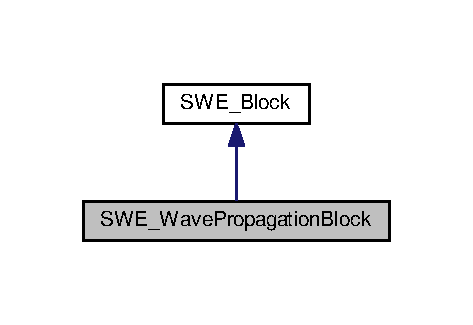
\includegraphics[width=227pt]{classSWE__WavePropagationBlock__inherit__graph}
\end{center}
\end{figure}


Collaboration diagram for S\+W\+E\+\_\+\+Wave\+Propagation\+Block\+:\nopagebreak
\begin{figure}[H]
\begin{center}
\leavevmode
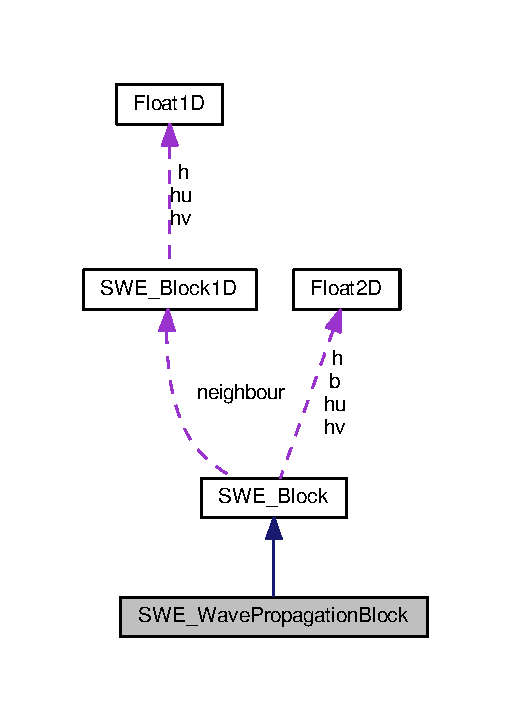
\includegraphics[width=245pt]{classSWE__WavePropagationBlock__coll__graph}
\end{center}
\end{figure}
\subsection*{Public Member Functions}
\begin{DoxyCompactItemize}
\item 
\hyperlink{classSWE__WavePropagationBlock_a9727e083d56a6d7aa9910f50c43080a9}{S\+W\+E\+\_\+\+Wave\+Propagation\+Block} (int l\+\_\+nx, int l\+\_\+ny, float l\+\_\+dx, float l\+\_\+dy)
\item 
void \hyperlink{classSWE__WavePropagationBlock_a5f6335a38fb3cf38623326959f06baf4}{compute\+Numerical\+Fluxes} ()
\item 
void \hyperlink{classSWE__WavePropagationBlock_a1b1422472a36602b34180e4ed27f6d8c}{update\+Unknowns} (float dt)
\item 
void \hyperlink{classSWE__WavePropagationBlock_ad7c91177190b9d131387998d16fa7df6}{update\+Unknowns\+Row} (float dt, int i)
\item 
virtual \hyperlink{classSWE__WavePropagationBlock_a9e53f3eaa7aee547ef88233069ff0667}{$\sim$\+S\+W\+E\+\_\+\+Wave\+Propagation\+Block} ()
\end{DoxyCompactItemize}
\subsection*{Additional Inherited Members}


\subsection{Detailed Description}
file is part of S\+WE 

\hyperlink{classSWE__WavePropagationBlock}{S\+W\+E\+\_\+\+Wave\+Propagation\+Block} is an implementation of the \hyperlink{classSWE__Block}{S\+W\+E\+\_\+\+Block} abstract class. It uses a wave propagation solver which is defined with the pre-\/compiler flag W\+A\+V\+E\+\_\+\+P\+R\+O\+P\+A\+G\+A\+T\+I\+O\+N\+\_\+\+S\+O\+L\+V\+ER (see above).

Possible wave propagation solvers are\+: F-\/\+Wave, Apprximate Augmented Riemann, Hybrid (f-\/wave + augmented). (details can be found in the corresponding source files) 

Definition at line 53 of file S\+W\+E\+\_\+\+Wave\+Propagation\+Block.\+hh.



\subsection{Constructor \& Destructor Documentation}
\index{S\+W\+E\+\_\+\+Wave\+Propagation\+Block@{S\+W\+E\+\_\+\+Wave\+Propagation\+Block}!S\+W\+E\+\_\+\+Wave\+Propagation\+Block@{S\+W\+E\+\_\+\+Wave\+Propagation\+Block}}
\index{S\+W\+E\+\_\+\+Wave\+Propagation\+Block@{S\+W\+E\+\_\+\+Wave\+Propagation\+Block}!S\+W\+E\+\_\+\+Wave\+Propagation\+Block@{S\+W\+E\+\_\+\+Wave\+Propagation\+Block}}
\subsubsection[{\texorpdfstring{S\+W\+E\+\_\+\+Wave\+Propagation\+Block(int l\+\_\+nx, int l\+\_\+ny, float l\+\_\+dx, float l\+\_\+dy)}{SWE_WavePropagationBlock(int l_nx, int l_ny, float l_dx, float l_dy)}}]{\setlength{\rightskip}{0pt plus 5cm}S\+W\+E\+\_\+\+Wave\+Propagation\+Block\+::\+S\+W\+E\+\_\+\+Wave\+Propagation\+Block (
\begin{DoxyParamCaption}
\item[{int}]{l\+\_\+nx, }
\item[{int}]{l\+\_\+ny, }
\item[{float}]{l\+\_\+dx, }
\item[{float}]{l\+\_\+dy}
\end{DoxyParamCaption}
)}\hypertarget{classSWE__WavePropagationBlock_a9727e083d56a6d7aa9910f50c43080a9}{}\label{classSWE__WavePropagationBlock_a9727e083d56a6d7aa9910f50c43080a9}
Constructor of a \hyperlink{classSWE__WavePropagationBlock}{S\+W\+E\+\_\+\+Wave\+Propagation\+Block}.

Allocates the variables for the simulation\+: unknowns h,hu,hv,b are defined on grid indices \mbox{[}0,..,nx+1\mbox{]}$\ast$\mbox{[}0,..,ny+1\mbox{]} (-\/$>$ Abstract class \hyperlink{classSWE__Block}{S\+W\+E\+\_\+\+Block}) -\/$>$ computational domain is \mbox{[}1,..,nx\mbox{]}$\ast$\mbox{[}1,..,ny\mbox{]} -\/$>$ plus ghost cell layer

net-\/updates are defined for edges with indices \mbox{[}0,..,nx\mbox{]}$\ast$\mbox{[}0,..,ny-\/1\mbox{]} or \mbox{[}0,..,nx-\/1\mbox{]}$\ast$\href{for horizontal/vertical edges}{\tt 0,..,ny}

A left/right net update with index (i-\/1,j-\/1) is located on the edge between cells with index (i-\/1,j) and (i,j)\+: 
\begin{DoxyPre}
  *********************
  *         *         *
  * (i-1,j) *  (i,j)  *
  *         *         *
  *********************\end{DoxyPre}



\begin{DoxyPre}            *
           ***
          *****
            *
            *
  NetUpdatesLeft(i-1,j-1)
            or
  NetUpdatesRight(i-1,j-1)
\end{DoxyPre}


A below/above net update with index (i-\/1, j-\/1) is located on the edge between cells with index (i, j-\/1) and (i,j)\+: 
\begin{DoxyPre}



  *         *
  * (i, j)  *   *
  *         *  **  NetUpdatesBelow(i-1,j-1)
  *********** *****         or
  *         *  **  NetUpdatesAbove(i-1,j-1)
  * (i,j-1) *   *
  *         *



\end{DoxyPre}
 

Definition at line 80 of file S\+W\+E\+\_\+\+Wave\+Propagation\+Block.\+cpp.

\index{S\+W\+E\+\_\+\+Wave\+Propagation\+Block@{S\+W\+E\+\_\+\+Wave\+Propagation\+Block}!````~S\+W\+E\+\_\+\+Wave\+Propagation\+Block@{$\sim$\+S\+W\+E\+\_\+\+Wave\+Propagation\+Block}}
\index{````~S\+W\+E\+\_\+\+Wave\+Propagation\+Block@{$\sim$\+S\+W\+E\+\_\+\+Wave\+Propagation\+Block}!S\+W\+E\+\_\+\+Wave\+Propagation\+Block@{S\+W\+E\+\_\+\+Wave\+Propagation\+Block}}
\subsubsection[{\texorpdfstring{$\sim$\+S\+W\+E\+\_\+\+Wave\+Propagation\+Block()}{~SWE_WavePropagationBlock()}}]{\setlength{\rightskip}{0pt plus 5cm}virtual S\+W\+E\+\_\+\+Wave\+Propagation\+Block\+::$\sim$\+S\+W\+E\+\_\+\+Wave\+Propagation\+Block (
\begin{DoxyParamCaption}
{}
\end{DoxyParamCaption}
)\hspace{0.3cm}{\ttfamily [inline]}, {\ttfamily [virtual]}}\hypertarget{classSWE__WavePropagationBlock_a9e53f3eaa7aee547ef88233069ff0667}{}\label{classSWE__WavePropagationBlock_a9e53f3eaa7aee547ef88233069ff0667}
Destructor of a \hyperlink{classSWE__WavePropagationBlock}{S\+W\+E\+\_\+\+Wave\+Propagation\+Block}.

In the case of a hybrid solver (N\+D\+E\+B\+UG not defined) information about the used solvers will be printed. 

Definition at line 97 of file S\+W\+E\+\_\+\+Wave\+Propagation\+Block.\+hh.



\subsection{Member Function Documentation}
\index{S\+W\+E\+\_\+\+Wave\+Propagation\+Block@{S\+W\+E\+\_\+\+Wave\+Propagation\+Block}!compute\+Numerical\+Fluxes@{compute\+Numerical\+Fluxes}}
\index{compute\+Numerical\+Fluxes@{compute\+Numerical\+Fluxes}!S\+W\+E\+\_\+\+Wave\+Propagation\+Block@{S\+W\+E\+\_\+\+Wave\+Propagation\+Block}}
\subsubsection[{\texorpdfstring{compute\+Numerical\+Fluxes()}{computeNumericalFluxes()}}]{\setlength{\rightskip}{0pt plus 5cm}void S\+W\+E\+\_\+\+Wave\+Propagation\+Block\+::compute\+Numerical\+Fluxes (
\begin{DoxyParamCaption}
{}
\end{DoxyParamCaption}
)\hspace{0.3cm}{\ttfamily [virtual]}}\hypertarget{classSWE__WavePropagationBlock_a5f6335a38fb3cf38623326959f06baf4}{}\label{classSWE__WavePropagationBlock_a5f6335a38fb3cf38623326959f06baf4}
Compute net updates for the block. The member variable \hyperlink{classSWE__Block_a05cbc9b40e0483bf73dbc2bdeae7dee3}{max\+Timestep} will be updated with the maximum allowed time step size 

Implements \hyperlink{classSWE__Block_a94dcf2c6ae31731e4586e45628b0c00e}{S\+W\+E\+\_\+\+Block}.



Definition at line 99 of file S\+W\+E\+\_\+\+Wave\+Propagation\+Block.\+cpp.

\index{S\+W\+E\+\_\+\+Wave\+Propagation\+Block@{S\+W\+E\+\_\+\+Wave\+Propagation\+Block}!update\+Unknowns@{update\+Unknowns}}
\index{update\+Unknowns@{update\+Unknowns}!S\+W\+E\+\_\+\+Wave\+Propagation\+Block@{S\+W\+E\+\_\+\+Wave\+Propagation\+Block}}
\subsubsection[{\texorpdfstring{update\+Unknowns(float dt)}{updateUnknowns(float dt)}}]{\setlength{\rightskip}{0pt plus 5cm}void S\+W\+E\+\_\+\+Wave\+Propagation\+Block\+::update\+Unknowns (
\begin{DoxyParamCaption}
\item[{float}]{dt}
\end{DoxyParamCaption}
)\hspace{0.3cm}{\ttfamily [virtual]}}\hypertarget{classSWE__WavePropagationBlock_a1b1422472a36602b34180e4ed27f6d8c}{}\label{classSWE__WavePropagationBlock_a1b1422472a36602b34180e4ed27f6d8c}
Updates the unknowns with the already computed net-\/updates.


\begin{DoxyParams}{Parameters}
{\em dt} & time step width used in the update. \\
\hline
\end{DoxyParams}


Implements \hyperlink{classSWE__Block_ab2b4b659f23d5d45413dece8d2da3298}{S\+W\+E\+\_\+\+Block}.



Definition at line 171 of file S\+W\+E\+\_\+\+Wave\+Propagation\+Block.\+cpp.

\index{S\+W\+E\+\_\+\+Wave\+Propagation\+Block@{S\+W\+E\+\_\+\+Wave\+Propagation\+Block}!update\+Unknowns\+Row@{update\+Unknowns\+Row}}
\index{update\+Unknowns\+Row@{update\+Unknowns\+Row}!S\+W\+E\+\_\+\+Wave\+Propagation\+Block@{S\+W\+E\+\_\+\+Wave\+Propagation\+Block}}
\subsubsection[{\texorpdfstring{update\+Unknowns\+Row(float dt, int i)}{updateUnknownsRow(float dt, int i)}}]{\setlength{\rightskip}{0pt plus 5cm}void S\+W\+E\+\_\+\+Wave\+Propagation\+Block\+::update\+Unknowns\+Row (
\begin{DoxyParamCaption}
\item[{float}]{dt, }
\item[{int}]{i}
\end{DoxyParamCaption}
)}\hypertarget{classSWE__WavePropagationBlock_ad7c91177190b9d131387998d16fa7df6}{}\label{classSWE__WavePropagationBlock_ad7c91177190b9d131387998d16fa7df6}


The documentation for this class was generated from the following files\+:\begin{DoxyCompactItemize}
\item 
app/src/main/cpp/blocks/\hyperlink{SWE__WavePropagationBlock_8hh}{S\+W\+E\+\_\+\+Wave\+Propagation\+Block.\+hh}\item 
app/src/main/cpp/blocks/\hyperlink{SWE__WavePropagationBlock_8cpp}{S\+W\+E\+\_\+\+Wave\+Propagation\+Block.\+cpp}\end{DoxyCompactItemize}

\hypertarget{classsolver_1_1WavePropagation}{}\section{solver\+:\+:Wave\+Propagation$<$ T $>$ Class Template Reference}
\label{classsolver_1_1WavePropagation}\index{solver\+::\+Wave\+Propagation$<$ T $>$@{solver\+::\+Wave\+Propagation$<$ T $>$}}


{\ttfamily \#include $<$Wave\+Propagation.\+hpp$>$}

\subsection*{Public Member Functions}
\begin{DoxyCompactItemize}
\item 
virtual void \hyperlink{classsolver_1_1WavePropagation_ace4a0a41b9003d0d7005226b81b982a4}{compute\+Net\+Updates} (const T \&i\+\_\+h\+Left, const T \&i\+\_\+h\+Right, const T \&i\+\_\+hu\+Left, const T \&i\+\_\+hu\+Right, const T \&i\+\_\+b\+Left, const T \&i\+\_\+b\+Right, T \&o\+\_\+h\+Update\+Left, T \&o\+\_\+h\+Update\+Right, T \&o\+\_\+hu\+Update\+Left, T \&o\+\_\+hu\+Update\+Right, T \&o\+\_\+max\+Wave\+Speed)=0
\item 
void \hyperlink{classsolver_1_1WavePropagation_a8f4fefb7e7fa823853b053edbcc53b12}{set\+Dry\+Tolerance} (const T i\+\_\+dry\+Tolerance)
\item 
virtual \hyperlink{classsolver_1_1WavePropagation_a2463938d462872abb6fca8fb88f04aa4}{$\sim$\+Wave\+Propagation} ()
\end{DoxyCompactItemize}
\subsection*{Protected Types}
\begin{DoxyCompactItemize}
\item 
enum \hyperlink{classsolver_1_1WavePropagation_a301203f09c080cff1f7f654ba04451cd}{Wet\+Dry\+State} \{ \\*
\hyperlink{classsolver_1_1WavePropagation_a301203f09c080cff1f7f654ba04451cda89ee27d8ba931e0b79f0f1b9ef0df3c1}{Dry\+Dry}, 
\hyperlink{classsolver_1_1WavePropagation_a301203f09c080cff1f7f654ba04451cda0ad584eeb02f684932bc0cd6608b5aea}{Wet\+Wet}, 
\hyperlink{classsolver_1_1WavePropagation_a301203f09c080cff1f7f654ba04451cda3ee9e6f341abb684450a39e2ccce7ac6}{Wet\+Dry\+Inundation}, 
\hyperlink{classsolver_1_1WavePropagation_a301203f09c080cff1f7f654ba04451cda2164f01921edc5f2a6663e105398ed57}{Wet\+Dry\+Wall}, 
\\*
\hyperlink{classsolver_1_1WavePropagation_a301203f09c080cff1f7f654ba04451cda6f680f0c1ab88d2d3a4706b74a2ebeae}{Wet\+Dry\+Wall\+Inundation}, 
\hyperlink{classsolver_1_1WavePropagation_a301203f09c080cff1f7f654ba04451cdac7251c834852f2ffa316c8d22d2f8b59}{Dry\+Wet\+Inundation}, 
\hyperlink{classsolver_1_1WavePropagation_a301203f09c080cff1f7f654ba04451cdaa862582670f74db35309b69f19745356}{Dry\+Wet\+Wall}, 
\hyperlink{classsolver_1_1WavePropagation_a301203f09c080cff1f7f654ba04451cdabd74beb894d60373cfd4f433da7c6a26}{Dry\+Wet\+Wall\+Inundation}
 \}
\end{DoxyCompactItemize}
\subsection*{Protected Member Functions}
\begin{DoxyCompactItemize}
\item 
virtual void \hyperlink{classsolver_1_1WavePropagation_accabfc2bea2eb577476d53c2117fd9d0}{determine\+Wet\+Dry\+State} ()=0
\begin{DoxyCompactList}\small\item\em Determine the wet/dry-\/state and set local values if we have to. \end{DoxyCompactList}\item 
\hyperlink{classsolver_1_1WavePropagation_ad99b3920e94402886323125e1bf39588}{Wave\+Propagation} (T i\+\_\+dry\+Tolerance, T i\+\_\+gravity, T i\+\_\+zero\+Tolerance)
\item 
void \hyperlink{classsolver_1_1WavePropagation_a1eed921157828ba1e5005e6f2c1709f7}{store\+Parameters} (const T \&i\+\_\+h\+Left, const T \&i\+\_\+h\+Right, const T \&i\+\_\+hu\+Left, const T \&i\+\_\+hu\+Right, const T \&i\+\_\+b\+Left, const T \&i\+\_\+b\+Right)
\item 
void \hyperlink{classsolver_1_1WavePropagation_a39e5490df673398dfb2f478b1b4b0d0e}{store\+Parameters} (const T \&i\+\_\+h\+Left, const T \&i\+\_\+h\+Right, const T \&i\+\_\+hu\+Left, const T \&i\+\_\+hu\+Right, const T \&i\+\_\+b\+Left, const T \&i\+\_\+b\+Right, const T \&i\+\_\+u\+Left, const T \&i\+\_\+u\+Right)
\end{DoxyCompactItemize}
\subsection*{Protected Attributes}
\begin{DoxyCompactItemize}
\item 
T \hyperlink{classsolver_1_1WavePropagation_a4a05c4bd71fdd1f8934ae5faddcea080}{dry\+Tol}
\begin{DoxyCompactList}\small\item\em numerical definition of \char`\"{}dry\char`\"{}. \end{DoxyCompactList}\item 
const T \hyperlink{classsolver_1_1WavePropagation_a5364825d416254d67103f1969ad2e273}{g}
\begin{DoxyCompactList}\small\item\em gravity constant \end{DoxyCompactList}\item 
const T \hyperlink{classsolver_1_1WavePropagation_ad49670e8fd53ef1ace084b618a0d9a02}{zero\+Tol}
\begin{DoxyCompactList}\small\item\em numerical definition of zero. \end{DoxyCompactList}\item 
T \hyperlink{classsolver_1_1WavePropagation_ae44e91bee496fad2170039ccdbb98743}{h\+Left}
\begin{DoxyCompactList}\small\item\em height on the left side of the edge (could change during execution). \end{DoxyCompactList}\item 
T \hyperlink{classsolver_1_1WavePropagation_a6269e7a67be3c63ceaca5a4030f921ec}{h\+Right}
\begin{DoxyCompactList}\small\item\em height on the right side of the edge (could change during execution). \end{DoxyCompactList}\item 
T \hyperlink{classsolver_1_1WavePropagation_a60c0a3d59b4e6225865f0442afbaa75d}{hu\+Left}
\begin{DoxyCompactList}\small\item\em momentum on the left side of the edge (could change during execution). \end{DoxyCompactList}\item 
T \hyperlink{classsolver_1_1WavePropagation_a511d65348b55c407e9ca909acadad555}{hu\+Right}
\begin{DoxyCompactList}\small\item\em momentum on the right side of the edge (could change during execution). \end{DoxyCompactList}\item 
T \hyperlink{classsolver_1_1WavePropagation_a809a5429a8d62ea7308611ed600ba679}{b\+Left}
\begin{DoxyCompactList}\small\item\em bathymetry on the left side of the edge (could change during execution). \end{DoxyCompactList}\item 
T \hyperlink{classsolver_1_1WavePropagation_a36a205e462d5775b7b343e25ab390e61}{b\+Right}
\begin{DoxyCompactList}\small\item\em bathymetry on the right side of the edge (could change during execution). \end{DoxyCompactList}\item 
T \hyperlink{classsolver_1_1WavePropagation_a987c0fc517379375f8120207a8af47d2}{u\+Left}
\begin{DoxyCompactList}\small\item\em velocity on the left side of the edge (computed by determine\+Wet\+Dry\+State). \end{DoxyCompactList}\item 
T \hyperlink{classsolver_1_1WavePropagation_a9689ef10a5ad6ab07054a34c9cdcc678}{u\+Right}
\begin{DoxyCompactList}\small\item\em velocity on the right side of the edge (computed by determine\+Wet\+Dry\+State). \end{DoxyCompactList}\item 
\hyperlink{classsolver_1_1WavePropagation_a301203f09c080cff1f7f654ba04451cd}{Wet\+Dry\+State} \hyperlink{classsolver_1_1WavePropagation_a5765dc8464b2046ac74631819b22c9eb}{wet\+Dry\+State}
\begin{DoxyCompactList}\small\item\em wet/dry state of our Riemann-\/problem (determined by determine\+Wet\+Dry\+State) \end{DoxyCompactList}\end{DoxyCompactItemize}


\subsection{Detailed Description}
\subsubsection*{template$<$typename T$>$\\*
class solver\+::\+Wave\+Propagation$<$ T $>$}



Definition at line 23 of file Wave\+Propagation.\+hpp.



\subsection{Member Enumeration Documentation}
\index{solver\+::\+Wave\+Propagation@{solver\+::\+Wave\+Propagation}!Wet\+Dry\+State@{Wet\+Dry\+State}}
\index{Wet\+Dry\+State@{Wet\+Dry\+State}!solver\+::\+Wave\+Propagation@{solver\+::\+Wave\+Propagation}}
\subsubsection[{\texorpdfstring{Wet\+Dry\+State}{WetDryState}}]{\setlength{\rightskip}{0pt plus 5cm}template$<$typename T $>$ enum {\bf solver\+::\+Wave\+Propagation\+::\+Wet\+Dry\+State}\hspace{0.3cm}{\ttfamily [protected]}}\hypertarget{classsolver_1_1WavePropagation_a301203f09c080cff1f7f654ba04451cd}{}\label{classsolver_1_1WavePropagation_a301203f09c080cff1f7f654ba04451cd}
The wet/dry state of the Riemann-\/problem. \begin{Desc}
\item[Enumerator]\par
\begin{description}
\index{Dry\+Dry@{Dry\+Dry}!solver\+::\+Wave\+Propagation@{solver\+::\+Wave\+Propagation}}\index{solver\+::\+Wave\+Propagation@{solver\+::\+Wave\+Propagation}!Dry\+Dry@{Dry\+Dry}}\item[{\em 
Dry\+Dry\hypertarget{classsolver_1_1WavePropagation_a301203f09c080cff1f7f654ba04451cda89ee27d8ba931e0b79f0f1b9ef0df3c1}{}\label{classsolver_1_1WavePropagation_a301203f09c080cff1f7f654ba04451cda89ee27d8ba931e0b79f0f1b9ef0df3c1}
}]Both cells are dry. \index{Wet\+Wet@{Wet\+Wet}!solver\+::\+Wave\+Propagation@{solver\+::\+Wave\+Propagation}}\index{solver\+::\+Wave\+Propagation@{solver\+::\+Wave\+Propagation}!Wet\+Wet@{Wet\+Wet}}\item[{\em 
Wet\+Wet\hypertarget{classsolver_1_1WavePropagation_a301203f09c080cff1f7f654ba04451cda0ad584eeb02f684932bc0cd6608b5aea}{}\label{classsolver_1_1WavePropagation_a301203f09c080cff1f7f654ba04451cda0ad584eeb02f684932bc0cd6608b5aea}
}]Both cells are wet. \index{Wet\+Dry\+Inundation@{Wet\+Dry\+Inundation}!solver\+::\+Wave\+Propagation@{solver\+::\+Wave\+Propagation}}\index{solver\+::\+Wave\+Propagation@{solver\+::\+Wave\+Propagation}!Wet\+Dry\+Inundation@{Wet\+Dry\+Inundation}}\item[{\em 
Wet\+Dry\+Inundation\hypertarget{classsolver_1_1WavePropagation_a301203f09c080cff1f7f654ba04451cda3ee9e6f341abb684450a39e2ccce7ac6}{}\label{classsolver_1_1WavePropagation_a301203f09c080cff1f7f654ba04451cda3ee9e6f341abb684450a39e2ccce7ac6}
}]1st cell\+: wet, 2nd cell\+: dry. 1st cell lies higher than the 2nd one. \index{Wet\+Dry\+Wall@{Wet\+Dry\+Wall}!solver\+::\+Wave\+Propagation@{solver\+::\+Wave\+Propagation}}\index{solver\+::\+Wave\+Propagation@{solver\+::\+Wave\+Propagation}!Wet\+Dry\+Wall@{Wet\+Dry\+Wall}}\item[{\em 
Wet\+Dry\+Wall\hypertarget{classsolver_1_1WavePropagation_a301203f09c080cff1f7f654ba04451cda2164f01921edc5f2a6663e105398ed57}{}\label{classsolver_1_1WavePropagation_a301203f09c080cff1f7f654ba04451cda2164f01921edc5f2a6663e105398ed57}
}]1st cell\+: wet, 2nd cell\+: dry. 1st cell lies lower than the 2nd one. Momentum is not large enough to overcome the difference. \index{Wet\+Dry\+Wall\+Inundation@{Wet\+Dry\+Wall\+Inundation}!solver\+::\+Wave\+Propagation@{solver\+::\+Wave\+Propagation}}\index{solver\+::\+Wave\+Propagation@{solver\+::\+Wave\+Propagation}!Wet\+Dry\+Wall\+Inundation@{Wet\+Dry\+Wall\+Inundation}}\item[{\em 
Wet\+Dry\+Wall\+Inundation\hypertarget{classsolver_1_1WavePropagation_a301203f09c080cff1f7f654ba04451cda6f680f0c1ab88d2d3a4706b74a2ebeae}{}\label{classsolver_1_1WavePropagation_a301203f09c080cff1f7f654ba04451cda6f680f0c1ab88d2d3a4706b74a2ebeae}
}]1st cell\+: wet, 2nd cell\+: dry. 1st cell lies lower than the 2nd one. Momentum is large enough to overcome the difference. \index{Dry\+Wet\+Inundation@{Dry\+Wet\+Inundation}!solver\+::\+Wave\+Propagation@{solver\+::\+Wave\+Propagation}}\index{solver\+::\+Wave\+Propagation@{solver\+::\+Wave\+Propagation}!Dry\+Wet\+Inundation@{Dry\+Wet\+Inundation}}\item[{\em 
Dry\+Wet\+Inundation\hypertarget{classsolver_1_1WavePropagation_a301203f09c080cff1f7f654ba04451cdac7251c834852f2ffa316c8d22d2f8b59}{}\label{classsolver_1_1WavePropagation_a301203f09c080cff1f7f654ba04451cdac7251c834852f2ffa316c8d22d2f8b59}
}]1st cell\+: dry, 2nd cell\+: wet. 1st cell lies lower than the 2nd one. \index{Dry\+Wet\+Wall@{Dry\+Wet\+Wall}!solver\+::\+Wave\+Propagation@{solver\+::\+Wave\+Propagation}}\index{solver\+::\+Wave\+Propagation@{solver\+::\+Wave\+Propagation}!Dry\+Wet\+Wall@{Dry\+Wet\+Wall}}\item[{\em 
Dry\+Wet\+Wall\hypertarget{classsolver_1_1WavePropagation_a301203f09c080cff1f7f654ba04451cdaa862582670f74db35309b69f19745356}{}\label{classsolver_1_1WavePropagation_a301203f09c080cff1f7f654ba04451cdaa862582670f74db35309b69f19745356}
}]1st cell\+: dry, 2nd cell\+: wet. 1st cell lies higher than the 2nd one. Momentum is not large enough to overcome the difference. \index{Dry\+Wet\+Wall\+Inundation@{Dry\+Wet\+Wall\+Inundation}!solver\+::\+Wave\+Propagation@{solver\+::\+Wave\+Propagation}}\index{solver\+::\+Wave\+Propagation@{solver\+::\+Wave\+Propagation}!Dry\+Wet\+Wall\+Inundation@{Dry\+Wet\+Wall\+Inundation}}\item[{\em 
Dry\+Wet\+Wall\+Inundation\hypertarget{classsolver_1_1WavePropagation_a301203f09c080cff1f7f654ba04451cdabd74beb894d60373cfd4f433da7c6a26}{}\label{classsolver_1_1WavePropagation_a301203f09c080cff1f7f654ba04451cdabd74beb894d60373cfd4f433da7c6a26}
}]1st cell\+: dry, 2nd cell\+: wet. 1st cell lies higher than the 2nd one. Momentum is large enough to overcome the difference. \end{description}
\end{Desc}


Definition at line 80 of file Wave\+Propagation.\+hpp.



\subsection{Constructor \& Destructor Documentation}
\index{solver\+::\+Wave\+Propagation@{solver\+::\+Wave\+Propagation}!Wave\+Propagation@{Wave\+Propagation}}
\index{Wave\+Propagation@{Wave\+Propagation}!solver\+::\+Wave\+Propagation@{solver\+::\+Wave\+Propagation}}
\subsubsection[{\texorpdfstring{Wave\+Propagation(\+T i\+\_\+dry\+Tolerance, T i\+\_\+gravity, T i\+\_\+zero\+Tolerance)}{WavePropagation(T i_dryTolerance, T i_gravity, T i_zeroTolerance)}}]{\setlength{\rightskip}{0pt plus 5cm}template$<$typename T $>$ {\bf solver\+::\+Wave\+Propagation}$<$ T $>$\+::{\bf Wave\+Propagation} (
\begin{DoxyParamCaption}
\item[{T}]{i\+\_\+dry\+Tolerance, }
\item[{T}]{i\+\_\+gravity, }
\item[{T}]{i\+\_\+zero\+Tolerance}
\end{DoxyParamCaption}
)\hspace{0.3cm}{\ttfamily [inline]}, {\ttfamily [protected]}}\hypertarget{classsolver_1_1WavePropagation_ad99b3920e94402886323125e1bf39588}{}\label{classsolver_1_1WavePropagation_ad99b3920e94402886323125e1bf39588}
Constructor of a wave propagation solver.


\begin{DoxyParams}{Parameters}
{\em gravity} & gravity constant. \\
\hline
{\em dry\+Tolerance} & numerical definition of \char`\"{}dry\char`\"{}. \\
\hline
{\em zero\+Tolerance} & numerical definition of zero. \\
\hline
\end{DoxyParams}


Definition at line 109 of file Wave\+Propagation.\+hpp.

\index{solver\+::\+Wave\+Propagation@{solver\+::\+Wave\+Propagation}!````~Wave\+Propagation@{$\sim$\+Wave\+Propagation}}
\index{````~Wave\+Propagation@{$\sim$\+Wave\+Propagation}!solver\+::\+Wave\+Propagation@{solver\+::\+Wave\+Propagation}}
\subsubsection[{\texorpdfstring{$\sim$\+Wave\+Propagation()}{~WavePropagation()}}]{\setlength{\rightskip}{0pt plus 5cm}template$<$typename T $>$ virtual {\bf solver\+::\+Wave\+Propagation}$<$ T $>$\+::$\sim${\bf Wave\+Propagation} (
\begin{DoxyParamCaption}
{}
\end{DoxyParamCaption}
)\hspace{0.3cm}{\ttfamily [inline]}, {\ttfamily [virtual]}}\hypertarget{classsolver_1_1WavePropagation_a2463938d462872abb6fca8fb88f04aa4}{}\label{classsolver_1_1WavePropagation_a2463938d462872abb6fca8fb88f04aa4}


Definition at line 206 of file Wave\+Propagation.\+hpp.



\subsection{Member Function Documentation}
\index{solver\+::\+Wave\+Propagation@{solver\+::\+Wave\+Propagation}!compute\+Net\+Updates@{compute\+Net\+Updates}}
\index{compute\+Net\+Updates@{compute\+Net\+Updates}!solver\+::\+Wave\+Propagation@{solver\+::\+Wave\+Propagation}}
\subsubsection[{\texorpdfstring{compute\+Net\+Updates(const T \&i\+\_\+h\+Left, const T \&i\+\_\+h\+Right, const T \&i\+\_\+hu\+Left, const T \&i\+\_\+hu\+Right, const T \&i\+\_\+b\+Left, const T \&i\+\_\+b\+Right, T \&o\+\_\+h\+Update\+Left, T \&o\+\_\+h\+Update\+Right, T \&o\+\_\+hu\+Update\+Left, T \&o\+\_\+hu\+Update\+Right, T \&o\+\_\+max\+Wave\+Speed)=0}{computeNetUpdates(const T &i_hLeft, const T &i_hRight, const T &i_huLeft, const T &i_huRight, const T &i_bLeft, const T &i_bRight, T &o_hUpdateLeft, T &o_hUpdateRight, T &o_huUpdateLeft, T &o_huUpdateRight, T &o_maxWaveSpeed)=0}}]{\setlength{\rightskip}{0pt plus 5cm}template$<$typename T $>$ virtual void {\bf solver\+::\+Wave\+Propagation}$<$ T $>$\+::compute\+Net\+Updates (
\begin{DoxyParamCaption}
\item[{const T \&}]{i\+\_\+h\+Left, }
\item[{const T \&}]{i\+\_\+h\+Right, }
\item[{const T \&}]{i\+\_\+hu\+Left, }
\item[{const T \&}]{i\+\_\+hu\+Right, }
\item[{const T \&}]{i\+\_\+b\+Left, }
\item[{const T \&}]{i\+\_\+b\+Right, }
\item[{T \&}]{o\+\_\+h\+Update\+Left, }
\item[{T \&}]{o\+\_\+h\+Update\+Right, }
\item[{T \&}]{o\+\_\+hu\+Update\+Left, }
\item[{T \&}]{o\+\_\+hu\+Update\+Right, }
\item[{T \&}]{o\+\_\+max\+Wave\+Speed}
\end{DoxyParamCaption}
)\hspace{0.3cm}{\ttfamily [pure virtual]}}\hypertarget{classsolver_1_1WavePropagation_ace4a0a41b9003d0d7005226b81b982a4}{}\label{classsolver_1_1WavePropagation_ace4a0a41b9003d0d7005226b81b982a4}
Compute net updates for the cell on the left/right side of the edge. This is the default method every standalone wave propagation solver should provide.


\begin{DoxyParams}{Parameters}
{\em i\+\_\+h\+Left} & height on the left side of the edge. \\
\hline
{\em i\+\_\+h\+Right} & height on the right side of the edge. \\
\hline
{\em i\+\_\+hu\+Left} & momentum on the left side of the edge. \\
\hline
{\em i\+\_\+hu\+Right} & momentum on the right side of the edge. \\
\hline
{\em i\+\_\+b\+Left} & bathymetry on the left side of the edge. \\
\hline
{\em i\+\_\+b\+Right} & bathymetry on the right side of the edge.\\
\hline
{\em o\+\_\+h\+Update\+Left} & will be set to\+: Net-\/update for the height of the cell on the left side of the edge. \\
\hline
{\em o\+\_\+h\+Update\+Right} & will be set to\+: Net-\/update for the height of the cell on the right side of the edge. \\
\hline
{\em o\+\_\+hu\+Update\+Left} & will be set to\+: Net-\/update for the momentum of the cell on the left side of the edge. \\
\hline
{\em o\+\_\+hu\+Update\+Right} & will be set to\+: Net-\/update for the momentum of the cell on the right side of the edge. \\
\hline
{\em o\+\_\+max\+Wave\+Speed} & will be set to\+: Maximum (linearized) wave speed -\/$>$ Should be used in the C\+F\+L-\/condition. \\
\hline
\end{DoxyParams}
\index{solver\+::\+Wave\+Propagation@{solver\+::\+Wave\+Propagation}!determine\+Wet\+Dry\+State@{determine\+Wet\+Dry\+State}}
\index{determine\+Wet\+Dry\+State@{determine\+Wet\+Dry\+State}!solver\+::\+Wave\+Propagation@{solver\+::\+Wave\+Propagation}}
\subsubsection[{\texorpdfstring{determine\+Wet\+Dry\+State()=0}{determineWetDryState()=0}}]{\setlength{\rightskip}{0pt plus 5cm}template$<$typename T $>$ virtual void {\bf solver\+::\+Wave\+Propagation}$<$ T $>$\+::determine\+Wet\+Dry\+State (
\begin{DoxyParamCaption}
{}
\end{DoxyParamCaption}
)\hspace{0.3cm}{\ttfamily [protected]}, {\ttfamily [pure virtual]}}\hypertarget{classsolver_1_1WavePropagation_accabfc2bea2eb577476d53c2117fd9d0}{}\label{classsolver_1_1WavePropagation_accabfc2bea2eb577476d53c2117fd9d0}


Determine the wet/dry-\/state and set local values if we have to. 

\index{solver\+::\+Wave\+Propagation@{solver\+::\+Wave\+Propagation}!set\+Dry\+Tolerance@{set\+Dry\+Tolerance}}
\index{set\+Dry\+Tolerance@{set\+Dry\+Tolerance}!solver\+::\+Wave\+Propagation@{solver\+::\+Wave\+Propagation}}
\subsubsection[{\texorpdfstring{set\+Dry\+Tolerance(const T i\+\_\+dry\+Tolerance)}{setDryTolerance(const T i_dryTolerance)}}]{\setlength{\rightskip}{0pt plus 5cm}template$<$typename T $>$ void {\bf solver\+::\+Wave\+Propagation}$<$ T $>$\+::set\+Dry\+Tolerance (
\begin{DoxyParamCaption}
\item[{const T}]{i\+\_\+dry\+Tolerance}
\end{DoxyParamCaption}
)\hspace{0.3cm}{\ttfamily [inline]}}\hypertarget{classsolver_1_1WavePropagation_a8f4fefb7e7fa823853b053edbcc53b12}{}\label{classsolver_1_1WavePropagation_a8f4fefb7e7fa823853b053edbcc53b12}
Sets the dry tolerance of the solver.


\begin{DoxyParams}{Parameters}
{\em i\+\_\+dry\+Tolerance} & dry tolerance. \\
\hline
\end{DoxyParams}


Definition at line 202 of file Wave\+Propagation.\+hpp.

\index{solver\+::\+Wave\+Propagation@{solver\+::\+Wave\+Propagation}!store\+Parameters@{store\+Parameters}}
\index{store\+Parameters@{store\+Parameters}!solver\+::\+Wave\+Propagation@{solver\+::\+Wave\+Propagation}}
\subsubsection[{\texorpdfstring{store\+Parameters(const T \&i\+\_\+h\+Left, const T \&i\+\_\+h\+Right, const T \&i\+\_\+hu\+Left, const T \&i\+\_\+hu\+Right, const T \&i\+\_\+b\+Left, const T \&i\+\_\+b\+Right)}{storeParameters(const T &i_hLeft, const T &i_hRight, const T &i_huLeft, const T &i_huRight, const T &i_bLeft, const T &i_bRight)}}]{\setlength{\rightskip}{0pt plus 5cm}template$<$typename T $>$ void {\bf solver\+::\+Wave\+Propagation}$<$ T $>$\+::store\+Parameters (
\begin{DoxyParamCaption}
\item[{const T \&}]{i\+\_\+h\+Left, }
\item[{const T \&}]{i\+\_\+h\+Right, }
\item[{const T \&}]{i\+\_\+hu\+Left, }
\item[{const T \&}]{i\+\_\+hu\+Right, }
\item[{const T \&}]{i\+\_\+b\+Left, }
\item[{const T \&}]{i\+\_\+b\+Right}
\end{DoxyParamCaption}
)\hspace{0.3cm}{\ttfamily [inline]}, {\ttfamily [protected]}}\hypertarget{classsolver_1_1WavePropagation_a1eed921157828ba1e5005e6f2c1709f7}{}\label{classsolver_1_1WavePropagation_a1eed921157828ba1e5005e6f2c1709f7}
Store parameters to member variables.


\begin{DoxyParams}{Parameters}
{\em i\+\_\+h\+Left} & height on the left side of the edge. \\
\hline
{\em i\+\_\+h\+Right} & height on the right side of the edge. \\
\hline
{\em i\+\_\+hu\+Left} & momentum on the left side of the edge. \\
\hline
{\em i\+\_\+hu\+Right} & momentum on the right side of the edge. \\
\hline
{\em i\+\_\+b\+Left} & bathymetry on the left side of the edge. \\
\hline
{\em i\+\_\+b\+Right} & bathymetry on the right side of the edge. \\
\hline
\end{DoxyParams}


Definition at line 126 of file Wave\+Propagation.\+hpp.

\index{solver\+::\+Wave\+Propagation@{solver\+::\+Wave\+Propagation}!store\+Parameters@{store\+Parameters}}
\index{store\+Parameters@{store\+Parameters}!solver\+::\+Wave\+Propagation@{solver\+::\+Wave\+Propagation}}
\subsubsection[{\texorpdfstring{store\+Parameters(const T \&i\+\_\+h\+Left, const T \&i\+\_\+h\+Right, const T \&i\+\_\+hu\+Left, const T \&i\+\_\+hu\+Right, const T \&i\+\_\+b\+Left, const T \&i\+\_\+b\+Right, const T \&i\+\_\+u\+Left, const T \&i\+\_\+u\+Right)}{storeParameters(const T &i_hLeft, const T &i_hRight, const T &i_huLeft, const T &i_huRight, const T &i_bLeft, const T &i_bRight, const T &i_uLeft, const T &i_uRight)}}]{\setlength{\rightskip}{0pt plus 5cm}template$<$typename T $>$ void {\bf solver\+::\+Wave\+Propagation}$<$ T $>$\+::store\+Parameters (
\begin{DoxyParamCaption}
\item[{const T \&}]{i\+\_\+h\+Left, }
\item[{const T \&}]{i\+\_\+h\+Right, }
\item[{const T \&}]{i\+\_\+hu\+Left, }
\item[{const T \&}]{i\+\_\+hu\+Right, }
\item[{const T \&}]{i\+\_\+b\+Left, }
\item[{const T \&}]{i\+\_\+b\+Right, }
\item[{const T \&}]{i\+\_\+u\+Left, }
\item[{const T \&}]{i\+\_\+u\+Right}
\end{DoxyParamCaption}
)\hspace{0.3cm}{\ttfamily [inline]}, {\ttfamily [protected]}}\hypertarget{classsolver_1_1WavePropagation_a39e5490df673398dfb2f478b1b4b0d0e}{}\label{classsolver_1_1WavePropagation_a39e5490df673398dfb2f478b1b4b0d0e}
Store parameters to member variables.


\begin{DoxyParams}{Parameters}
{\em i\+\_\+h\+Left} & height on the left side of the edge. \\
\hline
{\em i\+\_\+h\+Right} & height on the right side of the edge. \\
\hline
{\em i\+\_\+hu\+Left} & momentum on the left side of the edge. \\
\hline
{\em i\+\_\+hu\+Right} & momentum on the right side of the edge. \\
\hline
{\em i\+\_\+b\+Left} & bathymetry on the left side of the edge. \\
\hline
{\em i\+\_\+b\+Right} & bathymetry on the right side of the edge. \\
\hline
{\em i\+\_\+u\+Left} & velocity on the left side of the edge. \\
\hline
{\em i\+\_\+u\+Right} & velocity on the right side of the edge. \\
\hline
\end{DoxyParams}


Definition at line 152 of file Wave\+Propagation.\+hpp.



\subsection{Member Data Documentation}
\index{solver\+::\+Wave\+Propagation@{solver\+::\+Wave\+Propagation}!b\+Left@{b\+Left}}
\index{b\+Left@{b\+Left}!solver\+::\+Wave\+Propagation@{solver\+::\+Wave\+Propagation}}
\subsubsection[{\texorpdfstring{b\+Left}{bLeft}}]{\setlength{\rightskip}{0pt plus 5cm}template$<$typename T $>$ T {\bf solver\+::\+Wave\+Propagation}$<$ T $>$\+::b\+Left\hspace{0.3cm}{\ttfamily [protected]}}\hypertarget{classsolver_1_1WavePropagation_a809a5429a8d62ea7308611ed600ba679}{}\label{classsolver_1_1WavePropagation_a809a5429a8d62ea7308611ed600ba679}


bathymetry on the left side of the edge (could change during execution). 



Definition at line 67 of file Wave\+Propagation.\+hpp.

\index{solver\+::\+Wave\+Propagation@{solver\+::\+Wave\+Propagation}!b\+Right@{b\+Right}}
\index{b\+Right@{b\+Right}!solver\+::\+Wave\+Propagation@{solver\+::\+Wave\+Propagation}}
\subsubsection[{\texorpdfstring{b\+Right}{bRight}}]{\setlength{\rightskip}{0pt plus 5cm}template$<$typename T $>$ T {\bf solver\+::\+Wave\+Propagation}$<$ T $>$\+::b\+Right\hspace{0.3cm}{\ttfamily [protected]}}\hypertarget{classsolver_1_1WavePropagation_a36a205e462d5775b7b343e25ab390e61}{}\label{classsolver_1_1WavePropagation_a36a205e462d5775b7b343e25ab390e61}


bathymetry on the right side of the edge (could change during execution). 



Definition at line 69 of file Wave\+Propagation.\+hpp.

\index{solver\+::\+Wave\+Propagation@{solver\+::\+Wave\+Propagation}!dry\+Tol@{dry\+Tol}}
\index{dry\+Tol@{dry\+Tol}!solver\+::\+Wave\+Propagation@{solver\+::\+Wave\+Propagation}}
\subsubsection[{\texorpdfstring{dry\+Tol}{dryTol}}]{\setlength{\rightskip}{0pt plus 5cm}template$<$typename T $>$ T {\bf solver\+::\+Wave\+Propagation}$<$ T $>$\+::dry\+Tol\hspace{0.3cm}{\ttfamily [protected]}}\hypertarget{classsolver_1_1WavePropagation_a4a05c4bd71fdd1f8934ae5faddcea080}{}\label{classsolver_1_1WavePropagation_a4a05c4bd71fdd1f8934ae5faddcea080}


numerical definition of \char`\"{}dry\char`\"{}. 



Definition at line 31 of file Wave\+Propagation.\+hpp.

\index{solver\+::\+Wave\+Propagation@{solver\+::\+Wave\+Propagation}!g@{g}}
\index{g@{g}!solver\+::\+Wave\+Propagation@{solver\+::\+Wave\+Propagation}}
\subsubsection[{\texorpdfstring{g}{g}}]{\setlength{\rightskip}{0pt plus 5cm}template$<$typename T $>$ const T {\bf solver\+::\+Wave\+Propagation}$<$ T $>$\+::g\hspace{0.3cm}{\ttfamily [protected]}}\hypertarget{classsolver_1_1WavePropagation_a5364825d416254d67103f1969ad2e273}{}\label{classsolver_1_1WavePropagation_a5364825d416254d67103f1969ad2e273}


gravity constant 



Definition at line 33 of file Wave\+Propagation.\+hpp.

\index{solver\+::\+Wave\+Propagation@{solver\+::\+Wave\+Propagation}!h\+Left@{h\+Left}}
\index{h\+Left@{h\+Left}!solver\+::\+Wave\+Propagation@{solver\+::\+Wave\+Propagation}}
\subsubsection[{\texorpdfstring{h\+Left}{hLeft}}]{\setlength{\rightskip}{0pt plus 5cm}template$<$typename T $>$ T {\bf solver\+::\+Wave\+Propagation}$<$ T $>$\+::h\+Left\hspace{0.3cm}{\ttfamily [protected]}}\hypertarget{classsolver_1_1WavePropagation_ae44e91bee496fad2170039ccdbb98743}{}\label{classsolver_1_1WavePropagation_ae44e91bee496fad2170039ccdbb98743}


height on the left side of the edge (could change during execution). 



Definition at line 59 of file Wave\+Propagation.\+hpp.

\index{solver\+::\+Wave\+Propagation@{solver\+::\+Wave\+Propagation}!h\+Right@{h\+Right}}
\index{h\+Right@{h\+Right}!solver\+::\+Wave\+Propagation@{solver\+::\+Wave\+Propagation}}
\subsubsection[{\texorpdfstring{h\+Right}{hRight}}]{\setlength{\rightskip}{0pt plus 5cm}template$<$typename T $>$ T {\bf solver\+::\+Wave\+Propagation}$<$ T $>$\+::h\+Right\hspace{0.3cm}{\ttfamily [protected]}}\hypertarget{classsolver_1_1WavePropagation_a6269e7a67be3c63ceaca5a4030f921ec}{}\label{classsolver_1_1WavePropagation_a6269e7a67be3c63ceaca5a4030f921ec}


height on the right side of the edge (could change during execution). 



Definition at line 61 of file Wave\+Propagation.\+hpp.

\index{solver\+::\+Wave\+Propagation@{solver\+::\+Wave\+Propagation}!hu\+Left@{hu\+Left}}
\index{hu\+Left@{hu\+Left}!solver\+::\+Wave\+Propagation@{solver\+::\+Wave\+Propagation}}
\subsubsection[{\texorpdfstring{hu\+Left}{huLeft}}]{\setlength{\rightskip}{0pt plus 5cm}template$<$typename T $>$ T {\bf solver\+::\+Wave\+Propagation}$<$ T $>$\+::hu\+Left\hspace{0.3cm}{\ttfamily [protected]}}\hypertarget{classsolver_1_1WavePropagation_a60c0a3d59b4e6225865f0442afbaa75d}{}\label{classsolver_1_1WavePropagation_a60c0a3d59b4e6225865f0442afbaa75d}


momentum on the left side of the edge (could change during execution). 



Definition at line 63 of file Wave\+Propagation.\+hpp.

\index{solver\+::\+Wave\+Propagation@{solver\+::\+Wave\+Propagation}!hu\+Right@{hu\+Right}}
\index{hu\+Right@{hu\+Right}!solver\+::\+Wave\+Propagation@{solver\+::\+Wave\+Propagation}}
\subsubsection[{\texorpdfstring{hu\+Right}{huRight}}]{\setlength{\rightskip}{0pt plus 5cm}template$<$typename T $>$ T {\bf solver\+::\+Wave\+Propagation}$<$ T $>$\+::hu\+Right\hspace{0.3cm}{\ttfamily [protected]}}\hypertarget{classsolver_1_1WavePropagation_a511d65348b55c407e9ca909acadad555}{}\label{classsolver_1_1WavePropagation_a511d65348b55c407e9ca909acadad555}


momentum on the right side of the edge (could change during execution). 



Definition at line 65 of file Wave\+Propagation.\+hpp.

\index{solver\+::\+Wave\+Propagation@{solver\+::\+Wave\+Propagation}!u\+Left@{u\+Left}}
\index{u\+Left@{u\+Left}!solver\+::\+Wave\+Propagation@{solver\+::\+Wave\+Propagation}}
\subsubsection[{\texorpdfstring{u\+Left}{uLeft}}]{\setlength{\rightskip}{0pt plus 5cm}template$<$typename T $>$ T {\bf solver\+::\+Wave\+Propagation}$<$ T $>$\+::u\+Left\hspace{0.3cm}{\ttfamily [protected]}}\hypertarget{classsolver_1_1WavePropagation_a987c0fc517379375f8120207a8af47d2}{}\label{classsolver_1_1WavePropagation_a987c0fc517379375f8120207a8af47d2}


velocity on the left side of the edge (computed by determine\+Wet\+Dry\+State). 



Definition at line 72 of file Wave\+Propagation.\+hpp.

\index{solver\+::\+Wave\+Propagation@{solver\+::\+Wave\+Propagation}!u\+Right@{u\+Right}}
\index{u\+Right@{u\+Right}!solver\+::\+Wave\+Propagation@{solver\+::\+Wave\+Propagation}}
\subsubsection[{\texorpdfstring{u\+Right}{uRight}}]{\setlength{\rightskip}{0pt plus 5cm}template$<$typename T $>$ T {\bf solver\+::\+Wave\+Propagation}$<$ T $>$\+::u\+Right\hspace{0.3cm}{\ttfamily [protected]}}\hypertarget{classsolver_1_1WavePropagation_a9689ef10a5ad6ab07054a34c9cdcc678}{}\label{classsolver_1_1WavePropagation_a9689ef10a5ad6ab07054a34c9cdcc678}


velocity on the right side of the edge (computed by determine\+Wet\+Dry\+State). 



Definition at line 74 of file Wave\+Propagation.\+hpp.

\index{solver\+::\+Wave\+Propagation@{solver\+::\+Wave\+Propagation}!wet\+Dry\+State@{wet\+Dry\+State}}
\index{wet\+Dry\+State@{wet\+Dry\+State}!solver\+::\+Wave\+Propagation@{solver\+::\+Wave\+Propagation}}
\subsubsection[{\texorpdfstring{wet\+Dry\+State}{wetDryState}}]{\setlength{\rightskip}{0pt plus 5cm}template$<$typename T $>$ {\bf Wet\+Dry\+State} {\bf solver\+::\+Wave\+Propagation}$<$ T $>$\+::wet\+Dry\+State\hspace{0.3cm}{\ttfamily [protected]}}\hypertarget{classsolver_1_1WavePropagation_a5765dc8464b2046ac74631819b22c9eb}{}\label{classsolver_1_1WavePropagation_a5765dc8464b2046ac74631819b22c9eb}


wet/dry state of our Riemann-\/problem (determined by determine\+Wet\+Dry\+State) 



Definition at line 96 of file Wave\+Propagation.\+hpp.

\index{solver\+::\+Wave\+Propagation@{solver\+::\+Wave\+Propagation}!zero\+Tol@{zero\+Tol}}
\index{zero\+Tol@{zero\+Tol}!solver\+::\+Wave\+Propagation@{solver\+::\+Wave\+Propagation}}
\subsubsection[{\texorpdfstring{zero\+Tol}{zeroTol}}]{\setlength{\rightskip}{0pt plus 5cm}template$<$typename T $>$ const T {\bf solver\+::\+Wave\+Propagation}$<$ T $>$\+::zero\+Tol\hspace{0.3cm}{\ttfamily [protected]}}\hypertarget{classsolver_1_1WavePropagation_ad49670e8fd53ef1ace084b618a0d9a02}{}\label{classsolver_1_1WavePropagation_ad49670e8fd53ef1ace084b618a0d9a02}


numerical definition of zero. 



Definition at line 35 of file Wave\+Propagation.\+hpp.



The documentation for this class was generated from the following file\+:\begin{DoxyCompactItemize}
\item 
app/src/main/cpp/blocks/\hyperlink{WavePropagation_8hpp}{Wave\+Propagation.\+hpp}\end{DoxyCompactItemize}

\hypertarget{classWavePropagation}{}\section{Wave\+Propagation Class Reference}
\label{classWavePropagation}\index{Wave\+Propagation@{Wave\+Propagation}}


Abstract wave propagation solver for the Shallow Water Equations; T should be double or float;.  




\subsection{Detailed Description}
Abstract wave propagation solver for the Shallow Water Equations; T should be double or float;. 

The documentation for this class was generated from the following file\+:\begin{DoxyCompactItemize}
\item 
app/src/main/cpp/blocks/\hyperlink{WavePropagation_8hpp}{Wave\+Propagation.\+hpp}\end{DoxyCompactItemize}

\chapter{File Documentation}
\hypertarget{SWE__Block_8cpp}{}\section{app/src/main/cpp/blocks/\+S\+W\+E\+\_\+\+Block.cpp File Reference}
\label{SWE__Block_8cpp}\index{app/src/main/cpp/blocks/\+S\+W\+E\+\_\+\+Block.\+cpp@{app/src/main/cpp/blocks/\+S\+W\+E\+\_\+\+Block.\+cpp}}
{\ttfamily \#include \char`\"{}S\+W\+E\+\_\+\+Block.\+hh\char`\"{}}\\*
{\ttfamily \#include \char`\"{}../tools/help.\+hh\char`\"{}}\\*
{\ttfamily \#include $<$cmath$>$}\\*
{\ttfamily \#include $<$iostream$>$}\\*
{\ttfamily \#include $<$cassert$>$}\\*
{\ttfamily \#include $<$limits$>$}\\*
Include dependency graph for S\+W\+E\+\_\+\+Block.\+cpp\+:\nopagebreak
\begin{figure}[H]
\begin{center}
\leavevmode
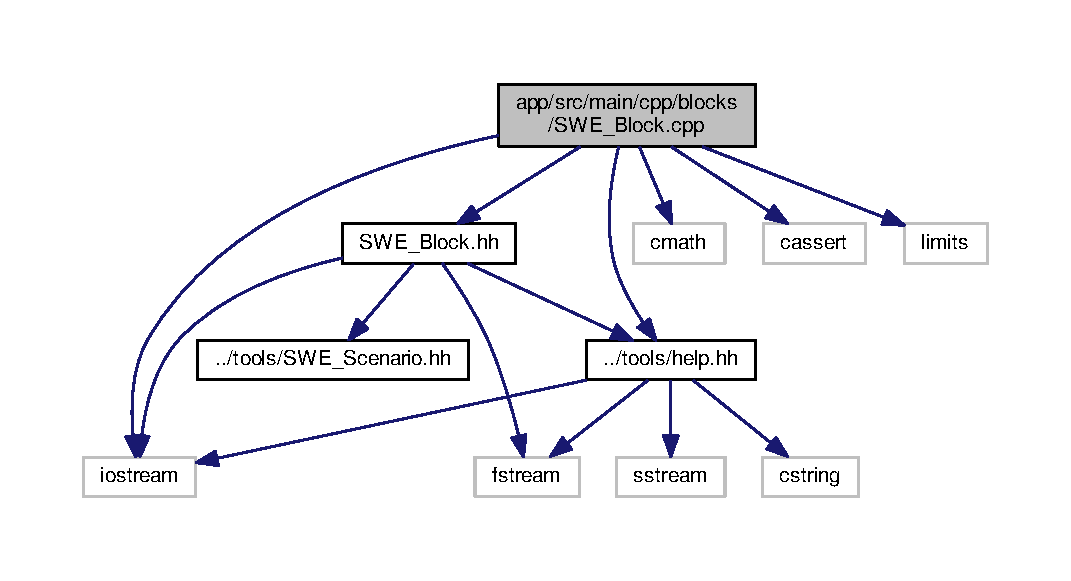
\includegraphics[width=350pt]{SWE__Block_8cpp__incl}
\end{center}
\end{figure}


\subsection{Detailed Description}
This file is part of S\+WE.

\begin{DoxyAuthor}{Author}
Michael Bader, Kaveh Rahnema, Tobias Schnabel 

Sebastian Rettenberger (rettenbs AT in.\+tum.\+de, \href{http://www5.in.tum.de/wiki/index.php/Sebastian_Rettenberger,_M.Sc}{\tt http\+://www5.\+in.\+tum.\+de/wiki/index.\+php/\+Sebastian\+\_\+\+Rettenberger,\+\_\+\+M.\+Sc}.)
\end{DoxyAuthor}
\hypertarget{help_8hh_LICENSE}{}\subsection{L\+I\+C\+E\+N\+SE}\label{help_8hh_LICENSE}
S\+WE is free software\+: you can redistribute it and/or modify it under the terms of the G\+NU General Public License as published by the Free Software Foundation, either version 3 of the License, or (at your option) any later version.

S\+WE is distributed in the hope that it will be useful, but W\+I\+T\+H\+O\+UT A\+NY W\+A\+R\+R\+A\+N\+TY; without even the implied warranty of M\+E\+R\+C\+H\+A\+N\+T\+A\+B\+I\+L\+I\+TY or F\+I\+T\+N\+E\+SS F\+OR A P\+A\+R\+T\+I\+C\+U\+L\+AR P\+U\+R\+P\+O\+SE. See the G\+NU General Public License for more details.

You should have received a copy of the G\+NU General Public License along with S\+WE. If not, see \href{http://www.gnu.org/licenses/}{\tt http\+://www.\+gnu.\+org/licenses/}.\hypertarget{help_8hh_DESCRIPTION}{}\subsection{D\+E\+S\+C\+R\+I\+P\+T\+I\+ON}\label{help_8hh_DESCRIPTION}
T\+O\+DO 
\hypertarget{SWE__Block_8hh}{}\section{app/src/main/cpp/blocks/\+S\+W\+E\+\_\+\+Block.hh File Reference}
\label{SWE__Block_8hh}\index{app/src/main/cpp/blocks/\+S\+W\+E\+\_\+\+Block.\+hh@{app/src/main/cpp/blocks/\+S\+W\+E\+\_\+\+Block.\+hh}}
{\ttfamily \#include \char`\"{}../tools/help.\+hh\char`\"{}}\\*
{\ttfamily \#include \char`\"{}../tools/\+S\+W\+E\+\_\+\+Scenario.\+hh\char`\"{}}\\*
{\ttfamily \#include $<$iostream$>$}\\*
{\ttfamily \#include $<$fstream$>$}\\*
Include dependency graph for S\+W\+E\+\_\+\+Block.\+hh\+:\nopagebreak
\begin{figure}[H]
\begin{center}
\leavevmode
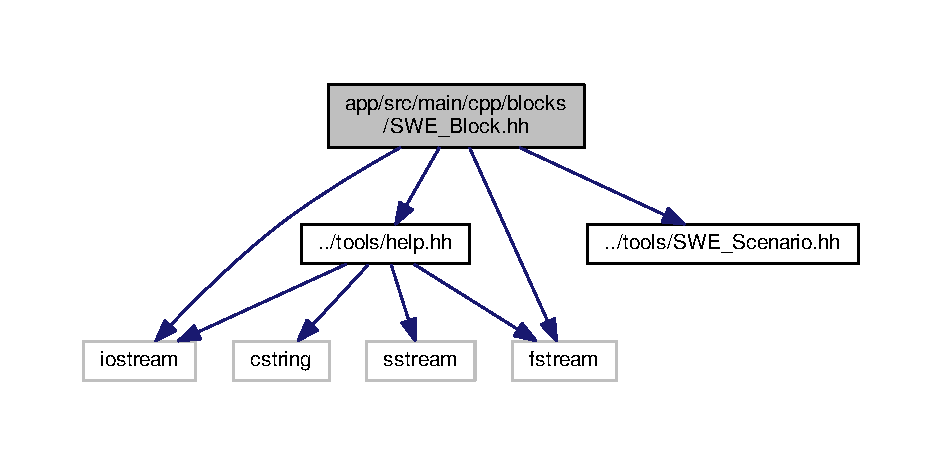
\includegraphics[width=350pt]{SWE__Block_8hh__incl}
\end{center}
\end{figure}
This graph shows which files directly or indirectly include this file\+:\nopagebreak
\begin{figure}[H]
\begin{center}
\leavevmode
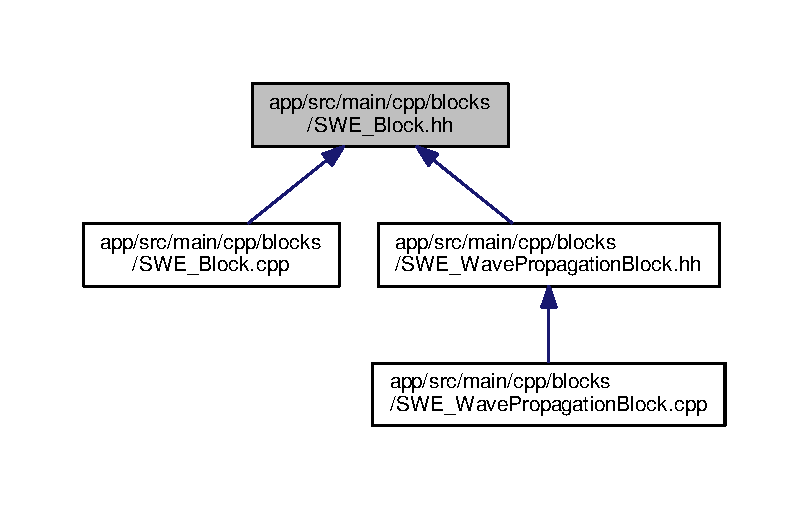
\includegraphics[width=350pt]{SWE__Block_8hh__dep__incl}
\end{center}
\end{figure}
\subsection*{Classes}
\begin{DoxyCompactItemize}
\item 
class \hyperlink{classSWE__Block}{S\+W\+E\+\_\+\+Block}
\begin{DoxyCompactList}\small\item\em This file is part of S\+WE. \end{DoxyCompactList}\item 
class \hyperlink{structSWE__Block1D}{S\+W\+E\+\_\+\+Block1D}
\begin{DoxyCompactList}\small\item\em This file is part S\+WE. \end{DoxyCompactList}\end{DoxyCompactItemize}


\subsection{Detailed Description}
This file is part of S\+WE.

\begin{DoxyAuthor}{Author}
Michael Bader, Kaveh Rahnema, Tobias Schnabel 

Sebastian Rettenberger (rettenbs AT in.\+tum.\+de, \href{http://www5.in.tum.de/wiki/index.php/Sebastian_Rettenberger,_M.Sc}{\tt http\+://www5.\+in.\+tum.\+de/wiki/index.\+php/\+Sebastian\+\_\+\+Rettenberger,\+\_\+\+M.\+Sc}.)
\end{DoxyAuthor}
\hypertarget{help_8hh_LICENSE}{}\subsection{L\+I\+C\+E\+N\+SE}\label{help_8hh_LICENSE}
S\+WE is free software\+: you can redistribute it and/or modify it under the terms of the G\+NU General Public License as published by the Free Software Foundation, either version 3 of the License, or (at your option) any later version.

S\+WE is distributed in the hope that it will be useful, but W\+I\+T\+H\+O\+UT A\+NY W\+A\+R\+R\+A\+N\+TY; without even the implied warranty of M\+E\+R\+C\+H\+A\+N\+T\+A\+B\+I\+L\+I\+TY or F\+I\+T\+N\+E\+SS F\+OR A P\+A\+R\+T\+I\+C\+U\+L\+AR P\+U\+R\+P\+O\+SE. See the G\+NU General Public License for more details.

You should have received a copy of the G\+NU General Public License along with S\+WE. If not, see \href{http://www.gnu.org/licenses/}{\tt http\+://www.\+gnu.\+org/licenses/}.\hypertarget{help_8hh_DESCRIPTION}{}\subsection{D\+E\+S\+C\+R\+I\+P\+T\+I\+ON}\label{help_8hh_DESCRIPTION}
T\+O\+DO 
\hypertarget{SWE__WavePropagationBlock_8cpp}{}\section{app/src/main/cpp/blocks/\+S\+W\+E\+\_\+\+Wave\+Propagation\+Block.cpp File Reference}
\label{SWE__WavePropagationBlock_8cpp}\index{app/src/main/cpp/blocks/\+S\+W\+E\+\_\+\+Wave\+Propagation\+Block.\+cpp@{app/src/main/cpp/blocks/\+S\+W\+E\+\_\+\+Wave\+Propagation\+Block.\+cpp}}
{\ttfamily \#include \char`\"{}S\+W\+E\+\_\+\+Wave\+Propagation\+Block.\+hh\char`\"{}}\\*
{\ttfamily \#include $<$string$>$}\\*
{\ttfamily \#include $<$limits$>$}\\*
Include dependency graph for S\+W\+E\+\_\+\+Wave\+Propagation\+Block.\+cpp\+:\nopagebreak
\begin{figure}[H]
\begin{center}
\leavevmode
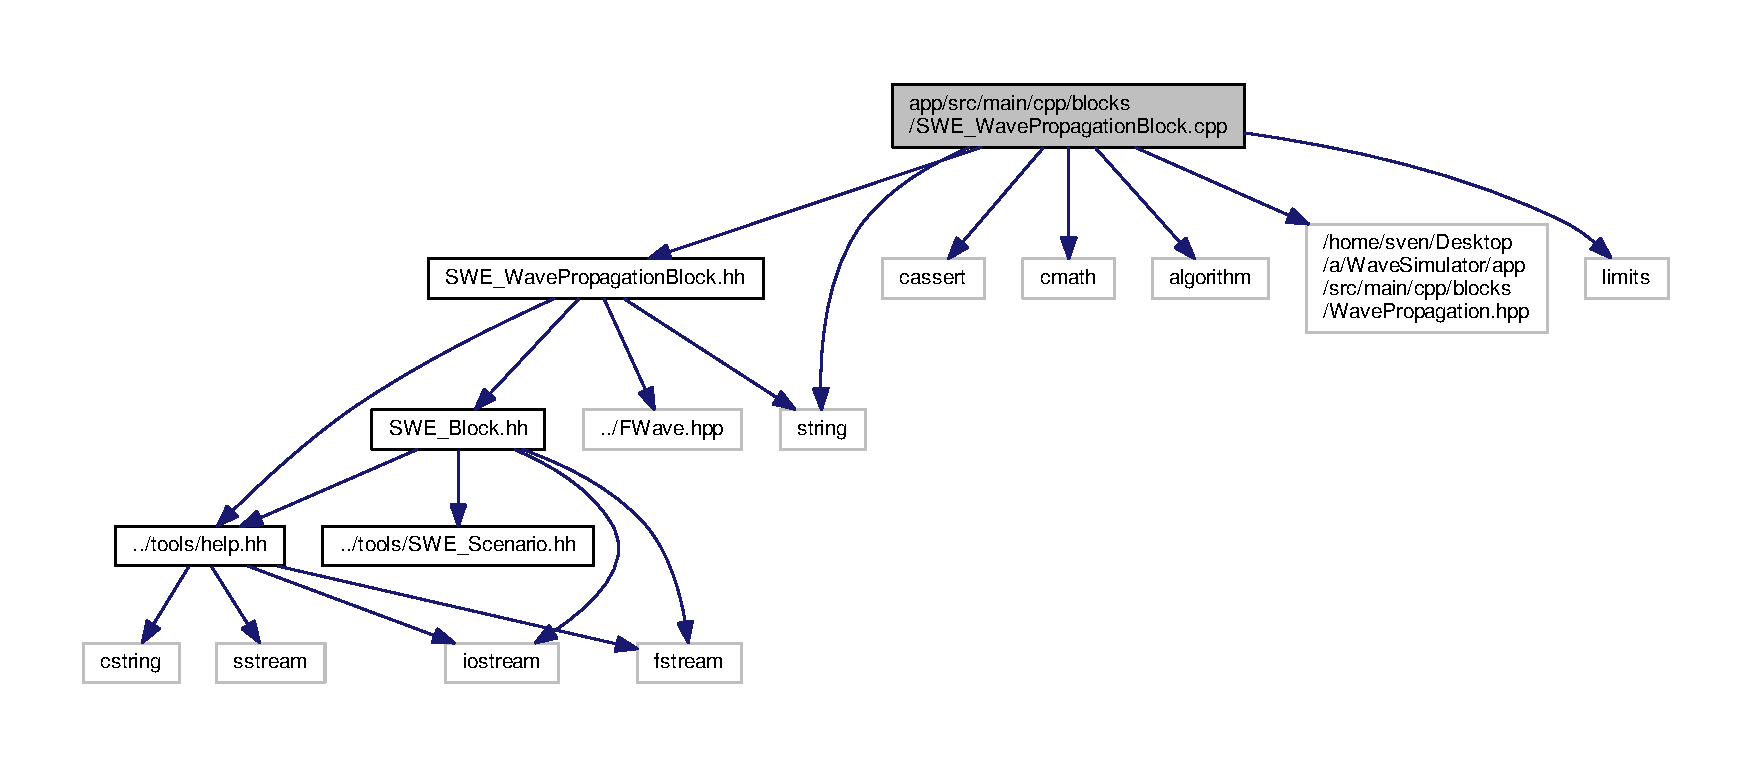
\includegraphics[width=350pt]{SWE__WavePropagationBlock_8cpp__incl}
\end{center}
\end{figure}


\subsection{Detailed Description}
This file is part of S\+WE.

\begin{DoxyAuthor}{Author}
Alexander Breuer (breuera AT in.\+tum.\+de, \href{http://www5.in.tum.de/wiki/index.php/Dipl.-Math._Alexander_Breuer}{\tt http\+://www5.\+in.\+tum.\+de/wiki/index.\+php/\+Dipl.-\/\+Math.\+\_\+\+Alexander\+\_\+\+Breuer}) 

Sebastian Rettenberger (rettenbs AT in.\+tum.\+de, \href{http://www5.in.tum.de/wiki/index.php/Sebastian_Rettenberger,_M.Sc}{\tt http\+://www5.\+in.\+tum.\+de/wiki/index.\+php/\+Sebastian\+\_\+\+Rettenberger,\+\_\+\+M.\+Sc}.) 

Michael Bader (bader AT in.\+tum.\+de, \href{http://www5.in.tum.de/wiki/index.php/Michael_Bader}{\tt http\+://www5.\+in.\+tum.\+de/wiki/index.\+php/\+Michael\+\_\+\+Bader})
\end{DoxyAuthor}
\hypertarget{help_8hh_LICENSE}{}\subsection{L\+I\+C\+E\+N\+SE}\label{help_8hh_LICENSE}
S\+WE is free software\+: you can redistribute it and/or modify it under the terms of the G\+NU General Public License as published by the Free Software Foundation, either version 3 of the License, or (at your option) any later version.

S\+WE is distributed in the hope that it will be useful, but W\+I\+T\+H\+O\+UT A\+NY W\+A\+R\+R\+A\+N\+TY; without even the implied warranty of M\+E\+R\+C\+H\+A\+N\+T\+A\+B\+I\+L\+I\+TY or F\+I\+T\+N\+E\+SS F\+OR A P\+A\+R\+T\+I\+C\+U\+L\+AR P\+U\+R\+P\+O\+SE. See the G\+NU General Public License for more details.

You should have received a copy of the G\+NU General Public License along with S\+WE. If not, see \href{http://www.gnu.org/licenses/}{\tt http\+://www.\+gnu.\+org/licenses/}.\hypertarget{help_8hh_DESCRIPTION}{}\subsection{D\+E\+S\+C\+R\+I\+P\+T\+I\+ON}\label{help_8hh_DESCRIPTION}
Implementation of \hyperlink{classSWE__Block}{S\+W\+E\+\_\+\+Block} that uses solvers in the wave propagation formulation. 
\hypertarget{SWE__WavePropagationBlock_8hh}{}\section{app/src/main/cpp/blocks/\+S\+W\+E\+\_\+\+Wave\+Propagation\+Block.hh File Reference}
\label{SWE__WavePropagationBlock_8hh}\index{app/src/main/cpp/blocks/\+S\+W\+E\+\_\+\+Wave\+Propagation\+Block.\+hh@{app/src/main/cpp/blocks/\+S\+W\+E\+\_\+\+Wave\+Propagation\+Block.\+hh}}
{\ttfamily \#include \char`\"{}S\+W\+E\+\_\+\+Block.\+hh\char`\"{}}\\*
{\ttfamily \#include \char`\"{}../tools/help.\+hh\char`\"{}}\\*
{\ttfamily \#include $<$string$>$}\\*
{\ttfamily \#include \char`\"{}../\+F\+Wave.\+hpp\char`\"{}}\\*
Include dependency graph for S\+W\+E\+\_\+\+Wave\+Propagation\+Block.\+hh\+:\nopagebreak
\begin{figure}[H]
\begin{center}
\leavevmode
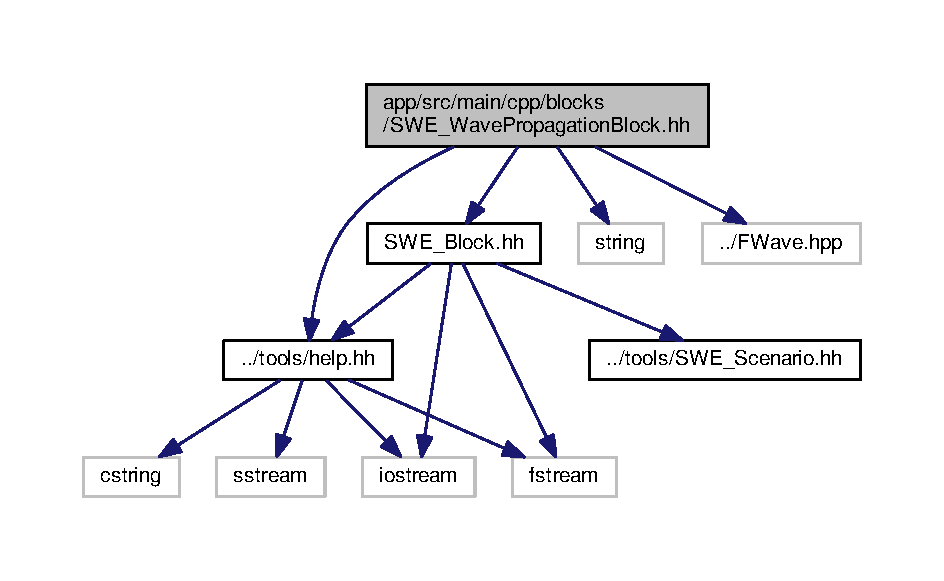
\includegraphics[width=350pt]{SWE__WavePropagationBlock_8hh__incl}
\end{center}
\end{figure}
This graph shows which files directly or indirectly include this file\+:\nopagebreak
\begin{figure}[H]
\begin{center}
\leavevmode
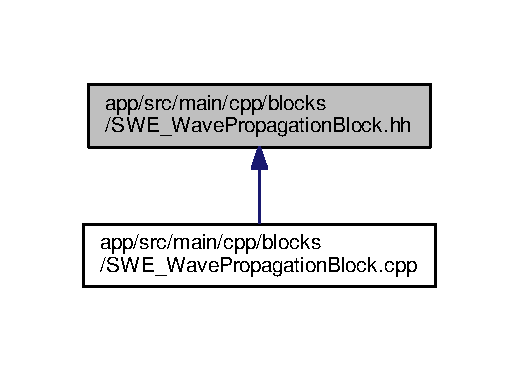
\includegraphics[width=249pt]{SWE__WavePropagationBlock_8hh__dep__incl}
\end{center}
\end{figure}
\subsection*{Classes}
\begin{DoxyCompactItemize}
\item 
class \hyperlink{classSWE__WavePropagationBlock}{S\+W\+E\+\_\+\+Wave\+Propagation\+Block}
\begin{DoxyCompactList}\small\item\em file is part of S\+WE \end{DoxyCompactList}\end{DoxyCompactItemize}


\subsection{Detailed Description}
This file is part of S\+WE.

\begin{DoxyAuthor}{Author}
Alexander Breuer (breuera AT in.\+tum.\+de, \href{http://www5.in.tum.de/wiki/index.php/Dipl.-Math._Alexander_Breuer}{\tt http\+://www5.\+in.\+tum.\+de/wiki/index.\+php/\+Dipl.-\/\+Math.\+\_\+\+Alexander\+\_\+\+Breuer}) 

Sebastian Rettenberger (rettenbs AT in.\+tum.\+de, \href{http://www5.in.tum.de/wiki/index.php/Sebastian_Rettenberger,_M.Sc}{\tt http\+://www5.\+in.\+tum.\+de/wiki/index.\+php/\+Sebastian\+\_\+\+Rettenberger,\+\_\+\+M.\+Sc}.) 

Michael Bader (bader AT in.\+tum.\+de, \href{http://www5.in.tum.de/wiki/index.php/Michael_Bader}{\tt http\+://www5.\+in.\+tum.\+de/wiki/index.\+php/\+Michael\+\_\+\+Bader})
\end{DoxyAuthor}
\hypertarget{help_8hh_LICENSE}{}\subsection{L\+I\+C\+E\+N\+SE}\label{help_8hh_LICENSE}
S\+WE is free software\+: you can redistribute it and/or modify it under the terms of the G\+NU General Public License as published by the Free Software Foundation, either version 3 of the License, or (at your option) any later version.

S\+WE is distributed in the hope that it will be useful, but W\+I\+T\+H\+O\+UT A\+NY W\+A\+R\+R\+A\+N\+TY; without even the implied warranty of M\+E\+R\+C\+H\+A\+N\+T\+A\+B\+I\+L\+I\+TY or F\+I\+T\+N\+E\+SS F\+OR A P\+A\+R\+T\+I\+C\+U\+L\+AR P\+U\+R\+P\+O\+SE. See the G\+NU General Public License for more details.

You should have received a copy of the G\+NU General Public License along with S\+WE. If not, see \href{http://www.gnu.org/licenses/}{\tt http\+://www.\+gnu.\+org/licenses/}.\hypertarget{help_8hh_DESCRIPTION}{}\subsection{D\+E\+S\+C\+R\+I\+P\+T\+I\+ON}\label{help_8hh_DESCRIPTION}
Implementation of \hyperlink{classSWE__Block}{S\+W\+E\+\_\+\+Block} that uses solvers in the wave propagation formulation. 
\hypertarget{WavePropagation_8cpp}{}\section{app/src/main/cpp/blocks/\+Wave\+Propagation.cpp File Reference}
\label{WavePropagation_8cpp}\index{app/src/main/cpp/blocks/\+Wave\+Propagation.\+cpp@{app/src/main/cpp/blocks/\+Wave\+Propagation.\+cpp}}
{\ttfamily \#include \char`\"{}Wave\+Propagation.\+hpp\char`\"{}}\\*
Include dependency graph for Wave\+Propagation.\+cpp\+:\nopagebreak
\begin{figure}[H]
\begin{center}
\leavevmode
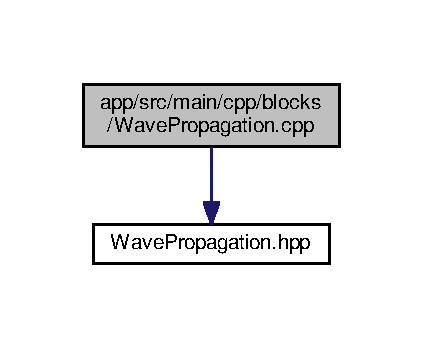
\includegraphics[width=203pt]{WavePropagation_8cpp__incl}
\end{center}
\end{figure}

\hypertarget{WavePropagation_8hpp}{}\section{app/src/main/cpp/blocks/\+Wave\+Propagation.hpp File Reference}
\label{WavePropagation_8hpp}\index{app/src/main/cpp/blocks/\+Wave\+Propagation.\+hpp@{app/src/main/cpp/blocks/\+Wave\+Propagation.\+hpp}}
This graph shows which files directly or indirectly include this file\+:\nopagebreak
\begin{figure}[H]
\begin{center}
\leavevmode
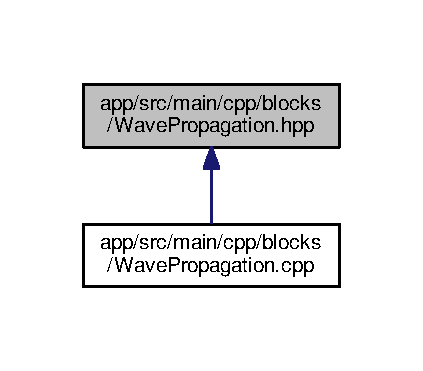
\includegraphics[width=203pt]{WavePropagation_8hpp__dep__incl}
\end{center}
\end{figure}
\subsection*{Classes}
\begin{DoxyCompactItemize}
\item 
class \hyperlink{classsolver_1_1WavePropagation}{solver\+::\+Wave\+Propagation$<$ T $>$}
\item 
class \hyperlink{classsolver_1_1WavePropagation}{solver\+::\+Wave\+Propagation$<$ T $>$}
\end{DoxyCompactItemize}
\subsection*{Namespaces}
\begin{DoxyCompactItemize}
\item 
 \hyperlink{namespacesolver}{solver}
\begin{DoxyCompactList}\small\item\em This namespace defines code that defines the S\+WE framework. \end{DoxyCompactList}\end{DoxyCompactItemize}

\hypertarget{scenarios_2SWE__Scenario_8hh}{}\section{app/src/main/cpp/scenarios/\+S\+W\+E\+\_\+\+Scenario.hh File Reference}
\label{scenarios_2SWE__Scenario_8hh}\index{app/src/main/cpp/scenarios/\+S\+W\+E\+\_\+\+Scenario.\+hh@{app/src/main/cpp/scenarios/\+S\+W\+E\+\_\+\+Scenario.\+hh}}
This graph shows which files directly or indirectly include this file\+:\nopagebreak
\begin{figure}[H]
\begin{center}
\leavevmode
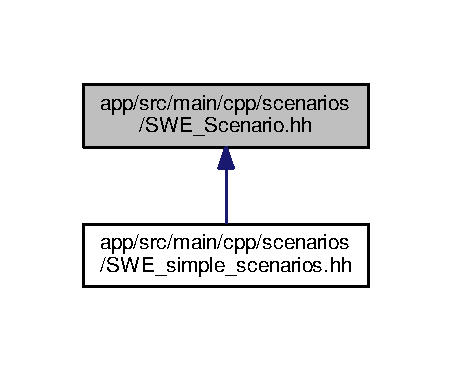
\includegraphics[width=217pt]{scenarios_2SWE__Scenario_8hh__dep__incl}
\end{center}
\end{figure}
\subsection*{Classes}
\begin{DoxyCompactItemize}
\item 
class \hyperlink{classSWE__Scenario}{S\+W\+E\+\_\+\+Scenario}
\begin{DoxyCompactList}\small\item\em This class sets the standart layout for all simulateable scenarios. \end{DoxyCompactList}\end{DoxyCompactItemize}
\subsection*{Typedefs}
\begin{DoxyCompactItemize}
\item 
typedef enum \hyperlink{scenarios_2SWE__Scenario_8hh_af75d5dd7322fa39ed0af4e7839e600f8}{Boundary\+Type} \hyperlink{scenarios_2SWE__Scenario_8hh_a0076a482278ddc13ed179c6c76c9b5ad}{Boundary\+Type}
\item 
typedef enum \hyperlink{scenarios_2SWE__Scenario_8hh_aa5e01e3f7df312f7b9b0d02521141fcc}{Boundary\+Edge} \hyperlink{scenarios_2SWE__Scenario_8hh_a53b43e70a19e542b4c1ab2da9c6bcc0e}{Boundary\+Edge}
\end{DoxyCompactItemize}
\subsection*{Enumerations}
\begin{DoxyCompactItemize}
\item 
enum \hyperlink{scenarios_2SWE__Scenario_8hh_af75d5dd7322fa39ed0af4e7839e600f8}{Boundary\+Type} \{ \\*
\hyperlink{scenarios_2SWE__Scenario_8hh_af75d5dd7322fa39ed0af4e7839e600f8abfcb976304836f3d329c3b7c8b7dbb63}{O\+U\+T\+F\+L\+OW}, 
\hyperlink{scenarios_2SWE__Scenario_8hh_af75d5dd7322fa39ed0af4e7839e600f8afca2faad41310c7e71ec303ef789c53a}{W\+A\+LL}, 
\hyperlink{scenarios_2SWE__Scenario_8hh_af75d5dd7322fa39ed0af4e7839e600f8a8c7e97da6bd5c3568ccc5ee6cd958c87}{I\+N\+F\+L\+OW}, 
\hyperlink{scenarios_2SWE__Scenario_8hh_af75d5dd7322fa39ed0af4e7839e600f8a20391dd2915a0e64343d24c2f2e40b95}{C\+O\+N\+N\+E\+CT}, 
\\*
\hyperlink{scenarios_2SWE__Scenario_8hh_af75d5dd7322fa39ed0af4e7839e600f8a48be352751e0dd34bbad624be5667ee2}{P\+A\+S\+S\+I\+VE}, 
\hyperlink{tools_2SWE__Scenario_8hh_af75d5dd7322fa39ed0af4e7839e600f8abfcb976304836f3d329c3b7c8b7dbb63}{O\+U\+T\+F\+L\+OW}, 
\hyperlink{tools_2SWE__Scenario_8hh_af75d5dd7322fa39ed0af4e7839e600f8afca2faad41310c7e71ec303ef789c53a}{W\+A\+LL}, 
\hyperlink{tools_2SWE__Scenario_8hh_af75d5dd7322fa39ed0af4e7839e600f8a8c7e97da6bd5c3568ccc5ee6cd958c87}{I\+N\+F\+L\+OW}, 
\\*
\hyperlink{tools_2SWE__Scenario_8hh_af75d5dd7322fa39ed0af4e7839e600f8a20391dd2915a0e64343d24c2f2e40b95}{C\+O\+N\+N\+E\+CT}, 
\hyperlink{tools_2SWE__Scenario_8hh_af75d5dd7322fa39ed0af4e7839e600f8a48be352751e0dd34bbad624be5667ee2}{P\+A\+S\+S\+I\+VE}
 \}
\item 
enum \hyperlink{scenarios_2SWE__Scenario_8hh_aa5e01e3f7df312f7b9b0d02521141fcc}{Boundary\+Edge} \{ \\*
\hyperlink{scenarios_2SWE__Scenario_8hh_aa5e01e3f7df312f7b9b0d02521141fcca34eeb3a076f3bbcb32d47b74ee3cee86}{B\+N\+D\+\_\+\+L\+E\+FT}, 
\hyperlink{scenarios_2SWE__Scenario_8hh_aa5e01e3f7df312f7b9b0d02521141fccac0391ea6a5bf43f7735142e9ae87a62f}{B\+N\+D\+\_\+\+R\+I\+G\+HT}, 
\hyperlink{scenarios_2SWE__Scenario_8hh_aa5e01e3f7df312f7b9b0d02521141fccaff0478ddcbdcce0a6af3a9dc75445380}{B\+N\+D\+\_\+\+B\+O\+T\+T\+OM}, 
\hyperlink{scenarios_2SWE__Scenario_8hh_aa5e01e3f7df312f7b9b0d02521141fcca80c82ce939775733d407d69e30f74177}{B\+N\+D\+\_\+\+T\+OP}, 
\\*
\hyperlink{tools_2SWE__Scenario_8hh_aa5e01e3f7df312f7b9b0d02521141fcca34eeb3a076f3bbcb32d47b74ee3cee86}{B\+N\+D\+\_\+\+L\+E\+FT}, 
\hyperlink{tools_2SWE__Scenario_8hh_aa5e01e3f7df312f7b9b0d02521141fccac0391ea6a5bf43f7735142e9ae87a62f}{B\+N\+D\+\_\+\+R\+I\+G\+HT}, 
\hyperlink{tools_2SWE__Scenario_8hh_aa5e01e3f7df312f7b9b0d02521141fccaff0478ddcbdcce0a6af3a9dc75445380}{B\+N\+D\+\_\+\+B\+O\+T\+T\+OM}, 
\hyperlink{tools_2SWE__Scenario_8hh_aa5e01e3f7df312f7b9b0d02521141fcca80c82ce939775733d407d69e30f74177}{B\+N\+D\+\_\+\+T\+OP}
 \}
\end{DoxyCompactItemize}


\subsection{Detailed Description}
This file is part of S\+WE.

\begin{DoxyAuthor}{Author}
Michael Bader, Kaveh Rahnema, Tobias Schnabel
\end{DoxyAuthor}
\hypertarget{help_8hh_LICENSE}{}\subsection{L\+I\+C\+E\+N\+SE}\label{help_8hh_LICENSE}
S\+WE is free software\+: you can redistribute it and/or modify it under the terms of the G\+NU General Public License as published by the Free Software Foundation, either version 3 of the License, or (at your option) any later version.

S\+WE is distributed in the hope that it will be useful, but W\+I\+T\+H\+O\+UT A\+NY W\+A\+R\+R\+A\+N\+TY; without even the implied warranty of M\+E\+R\+C\+H\+A\+N\+T\+A\+B\+I\+L\+I\+TY or F\+I\+T\+N\+E\+SS F\+OR A P\+A\+R\+T\+I\+C\+U\+L\+AR P\+U\+R\+P\+O\+SE. See the G\+NU General Public License for more details.

You should have received a copy of the G\+NU General Public License along with S\+WE. If not, see \href{http://www.gnu.org/licenses/}{\tt http\+://www.\+gnu.\+org/licenses/}.\hypertarget{help_8hh_DESCRIPTION}{}\subsection{D\+E\+S\+C\+R\+I\+P\+T\+I\+ON}\label{help_8hh_DESCRIPTION}
T\+O\+DO 

\subsection{Typedef Documentation}
\index{scenarios/\+S\+W\+E\+\_\+\+Scenario.\+hh@{scenarios/\+S\+W\+E\+\_\+\+Scenario.\+hh}!Boundary\+Edge@{Boundary\+Edge}}
\index{Boundary\+Edge@{Boundary\+Edge}!scenarios/\+S\+W\+E\+\_\+\+Scenario.\+hh@{scenarios/\+S\+W\+E\+\_\+\+Scenario.\+hh}}
\subsubsection[{\texorpdfstring{Boundary\+Edge}{BoundaryEdge}}]{\setlength{\rightskip}{0pt plus 5cm}typedef enum {\bf Boundary\+Edge}  {\bf Boundary\+Edge}}\hypertarget{scenarios_2SWE__Scenario_8hh_a53b43e70a19e542b4c1ab2da9c6bcc0e}{}\label{scenarios_2SWE__Scenario_8hh_a53b43e70a19e542b4c1ab2da9c6bcc0e}
enum type\+: numbering of the boundary edges \index{scenarios/\+S\+W\+E\+\_\+\+Scenario.\+hh@{scenarios/\+S\+W\+E\+\_\+\+Scenario.\+hh}!Boundary\+Type@{Boundary\+Type}}
\index{Boundary\+Type@{Boundary\+Type}!scenarios/\+S\+W\+E\+\_\+\+Scenario.\+hh@{scenarios/\+S\+W\+E\+\_\+\+Scenario.\+hh}}
\subsubsection[{\texorpdfstring{Boundary\+Type}{BoundaryType}}]{\setlength{\rightskip}{0pt plus 5cm}typedef enum {\bf Boundary\+Type}  {\bf Boundary\+Type}}\hypertarget{scenarios_2SWE__Scenario_8hh_a0076a482278ddc13ed179c6c76c9b5ad}{}\label{scenarios_2SWE__Scenario_8hh_a0076a482278ddc13ed179c6c76c9b5ad}
enum type\+: available types of boundary conditions 

\subsection{Enumeration Type Documentation}
\index{scenarios/\+S\+W\+E\+\_\+\+Scenario.\+hh@{scenarios/\+S\+W\+E\+\_\+\+Scenario.\+hh}!Boundary\+Edge@{Boundary\+Edge}}
\index{Boundary\+Edge@{Boundary\+Edge}!scenarios/\+S\+W\+E\+\_\+\+Scenario.\+hh@{scenarios/\+S\+W\+E\+\_\+\+Scenario.\+hh}}
\subsubsection[{\texorpdfstring{Boundary\+Edge}{BoundaryEdge}}]{\setlength{\rightskip}{0pt plus 5cm}enum {\bf Boundary\+Edge}}\hypertarget{scenarios_2SWE__Scenario_8hh_aa5e01e3f7df312f7b9b0d02521141fcc}{}\label{scenarios_2SWE__Scenario_8hh_aa5e01e3f7df312f7b9b0d02521141fcc}
enum type\+: numbering of the boundary edges \begin{Desc}
\item[Enumerator]\par
\begin{description}
\index{B\+N\+D\+\_\+\+L\+E\+FT@{B\+N\+D\+\_\+\+L\+E\+FT}!scenarios/\+S\+W\+E\+\_\+\+Scenario.\+hh@{scenarios/\+S\+W\+E\+\_\+\+Scenario.\+hh}}\index{scenarios/\+S\+W\+E\+\_\+\+Scenario.\+hh@{scenarios/\+S\+W\+E\+\_\+\+Scenario.\+hh}!B\+N\+D\+\_\+\+L\+E\+FT@{B\+N\+D\+\_\+\+L\+E\+FT}}\item[{\em 
B\+N\+D\+\_\+\+L\+E\+FT\hypertarget{scenarios_2SWE__Scenario_8hh_aa5e01e3f7df312f7b9b0d02521141fcca34eeb3a076f3bbcb32d47b74ee3cee86}{}\label{scenarios_2SWE__Scenario_8hh_aa5e01e3f7df312f7b9b0d02521141fcca34eeb3a076f3bbcb32d47b74ee3cee86}
}]\index{B\+N\+D\+\_\+\+R\+I\+G\+HT@{B\+N\+D\+\_\+\+R\+I\+G\+HT}!scenarios/\+S\+W\+E\+\_\+\+Scenario.\+hh@{scenarios/\+S\+W\+E\+\_\+\+Scenario.\+hh}}\index{scenarios/\+S\+W\+E\+\_\+\+Scenario.\+hh@{scenarios/\+S\+W\+E\+\_\+\+Scenario.\+hh}!B\+N\+D\+\_\+\+R\+I\+G\+HT@{B\+N\+D\+\_\+\+R\+I\+G\+HT}}\item[{\em 
B\+N\+D\+\_\+\+R\+I\+G\+HT\hypertarget{scenarios_2SWE__Scenario_8hh_aa5e01e3f7df312f7b9b0d02521141fccac0391ea6a5bf43f7735142e9ae87a62f}{}\label{scenarios_2SWE__Scenario_8hh_aa5e01e3f7df312f7b9b0d02521141fccac0391ea6a5bf43f7735142e9ae87a62f}
}]\index{B\+N\+D\+\_\+\+B\+O\+T\+T\+OM@{B\+N\+D\+\_\+\+B\+O\+T\+T\+OM}!scenarios/\+S\+W\+E\+\_\+\+Scenario.\+hh@{scenarios/\+S\+W\+E\+\_\+\+Scenario.\+hh}}\index{scenarios/\+S\+W\+E\+\_\+\+Scenario.\+hh@{scenarios/\+S\+W\+E\+\_\+\+Scenario.\+hh}!B\+N\+D\+\_\+\+B\+O\+T\+T\+OM@{B\+N\+D\+\_\+\+B\+O\+T\+T\+OM}}\item[{\em 
B\+N\+D\+\_\+\+B\+O\+T\+T\+OM\hypertarget{scenarios_2SWE__Scenario_8hh_aa5e01e3f7df312f7b9b0d02521141fccaff0478ddcbdcce0a6af3a9dc75445380}{}\label{scenarios_2SWE__Scenario_8hh_aa5e01e3f7df312f7b9b0d02521141fccaff0478ddcbdcce0a6af3a9dc75445380}
}]\index{B\+N\+D\+\_\+\+T\+OP@{B\+N\+D\+\_\+\+T\+OP}!scenarios/\+S\+W\+E\+\_\+\+Scenario.\+hh@{scenarios/\+S\+W\+E\+\_\+\+Scenario.\+hh}}\index{scenarios/\+S\+W\+E\+\_\+\+Scenario.\+hh@{scenarios/\+S\+W\+E\+\_\+\+Scenario.\+hh}!B\+N\+D\+\_\+\+T\+OP@{B\+N\+D\+\_\+\+T\+OP}}\item[{\em 
B\+N\+D\+\_\+\+T\+OP\hypertarget{scenarios_2SWE__Scenario_8hh_aa5e01e3f7df312f7b9b0d02521141fcca80c82ce939775733d407d69e30f74177}{}\label{scenarios_2SWE__Scenario_8hh_aa5e01e3f7df312f7b9b0d02521141fcca80c82ce939775733d407d69e30f74177}
}]\index{B\+N\+D\+\_\+\+L\+E\+FT@{B\+N\+D\+\_\+\+L\+E\+FT}!scenarios/\+S\+W\+E\+\_\+\+Scenario.\+hh@{scenarios/\+S\+W\+E\+\_\+\+Scenario.\+hh}}\index{scenarios/\+S\+W\+E\+\_\+\+Scenario.\+hh@{scenarios/\+S\+W\+E\+\_\+\+Scenario.\+hh}!B\+N\+D\+\_\+\+L\+E\+FT@{B\+N\+D\+\_\+\+L\+E\+FT}}\item[{\em 
B\+N\+D\+\_\+\+L\+E\+FT\hypertarget{scenarios_2SWE__Scenario_8hh_aa5e01e3f7df312f7b9b0d02521141fcca34eeb3a076f3bbcb32d47b74ee3cee86}{}\label{scenarios_2SWE__Scenario_8hh_aa5e01e3f7df312f7b9b0d02521141fcca34eeb3a076f3bbcb32d47b74ee3cee86}
}]\index{B\+N\+D\+\_\+\+R\+I\+G\+HT@{B\+N\+D\+\_\+\+R\+I\+G\+HT}!scenarios/\+S\+W\+E\+\_\+\+Scenario.\+hh@{scenarios/\+S\+W\+E\+\_\+\+Scenario.\+hh}}\index{scenarios/\+S\+W\+E\+\_\+\+Scenario.\+hh@{scenarios/\+S\+W\+E\+\_\+\+Scenario.\+hh}!B\+N\+D\+\_\+\+R\+I\+G\+HT@{B\+N\+D\+\_\+\+R\+I\+G\+HT}}\item[{\em 
B\+N\+D\+\_\+\+R\+I\+G\+HT\hypertarget{scenarios_2SWE__Scenario_8hh_aa5e01e3f7df312f7b9b0d02521141fccac0391ea6a5bf43f7735142e9ae87a62f}{}\label{scenarios_2SWE__Scenario_8hh_aa5e01e3f7df312f7b9b0d02521141fccac0391ea6a5bf43f7735142e9ae87a62f}
}]\index{B\+N\+D\+\_\+\+B\+O\+T\+T\+OM@{B\+N\+D\+\_\+\+B\+O\+T\+T\+OM}!scenarios/\+S\+W\+E\+\_\+\+Scenario.\+hh@{scenarios/\+S\+W\+E\+\_\+\+Scenario.\+hh}}\index{scenarios/\+S\+W\+E\+\_\+\+Scenario.\+hh@{scenarios/\+S\+W\+E\+\_\+\+Scenario.\+hh}!B\+N\+D\+\_\+\+B\+O\+T\+T\+OM@{B\+N\+D\+\_\+\+B\+O\+T\+T\+OM}}\item[{\em 
B\+N\+D\+\_\+\+B\+O\+T\+T\+OM\hypertarget{scenarios_2SWE__Scenario_8hh_aa5e01e3f7df312f7b9b0d02521141fccaff0478ddcbdcce0a6af3a9dc75445380}{}\label{scenarios_2SWE__Scenario_8hh_aa5e01e3f7df312f7b9b0d02521141fccaff0478ddcbdcce0a6af3a9dc75445380}
}]\index{B\+N\+D\+\_\+\+T\+OP@{B\+N\+D\+\_\+\+T\+OP}!scenarios/\+S\+W\+E\+\_\+\+Scenario.\+hh@{scenarios/\+S\+W\+E\+\_\+\+Scenario.\+hh}}\index{scenarios/\+S\+W\+E\+\_\+\+Scenario.\+hh@{scenarios/\+S\+W\+E\+\_\+\+Scenario.\+hh}!B\+N\+D\+\_\+\+T\+OP@{B\+N\+D\+\_\+\+T\+OP}}\item[{\em 
B\+N\+D\+\_\+\+T\+OP\hypertarget{scenarios_2SWE__Scenario_8hh_aa5e01e3f7df312f7b9b0d02521141fcca80c82ce939775733d407d69e30f74177}{}\label{scenarios_2SWE__Scenario_8hh_aa5e01e3f7df312f7b9b0d02521141fcca80c82ce939775733d407d69e30f74177}
}]\end{description}
\end{Desc}


Definition at line 41 of file S\+W\+E\+\_\+\+Scenario.\+hh.

\index{scenarios/\+S\+W\+E\+\_\+\+Scenario.\+hh@{scenarios/\+S\+W\+E\+\_\+\+Scenario.\+hh}!Boundary\+Type@{Boundary\+Type}}
\index{Boundary\+Type@{Boundary\+Type}!scenarios/\+S\+W\+E\+\_\+\+Scenario.\+hh@{scenarios/\+S\+W\+E\+\_\+\+Scenario.\+hh}}
\subsubsection[{\texorpdfstring{Boundary\+Type}{BoundaryType}}]{\setlength{\rightskip}{0pt plus 5cm}enum {\bf Boundary\+Type}}\hypertarget{scenarios_2SWE__Scenario_8hh_af75d5dd7322fa39ed0af4e7839e600f8}{}\label{scenarios_2SWE__Scenario_8hh_af75d5dd7322fa39ed0af4e7839e600f8}
enum type\+: available types of boundary conditions \begin{Desc}
\item[Enumerator]\par
\begin{description}
\index{O\+U\+T\+F\+L\+OW@{O\+U\+T\+F\+L\+OW}!scenarios/\+S\+W\+E\+\_\+\+Scenario.\+hh@{scenarios/\+S\+W\+E\+\_\+\+Scenario.\+hh}}\index{scenarios/\+S\+W\+E\+\_\+\+Scenario.\+hh@{scenarios/\+S\+W\+E\+\_\+\+Scenario.\+hh}!O\+U\+T\+F\+L\+OW@{O\+U\+T\+F\+L\+OW}}\item[{\em 
O\+U\+T\+F\+L\+OW\hypertarget{scenarios_2SWE__Scenario_8hh_af75d5dd7322fa39ed0af4e7839e600f8abfcb976304836f3d329c3b7c8b7dbb63}{}\label{scenarios_2SWE__Scenario_8hh_af75d5dd7322fa39ed0af4e7839e600f8abfcb976304836f3d329c3b7c8b7dbb63}
}]\index{W\+A\+LL@{W\+A\+LL}!scenarios/\+S\+W\+E\+\_\+\+Scenario.\+hh@{scenarios/\+S\+W\+E\+\_\+\+Scenario.\+hh}}\index{scenarios/\+S\+W\+E\+\_\+\+Scenario.\+hh@{scenarios/\+S\+W\+E\+\_\+\+Scenario.\+hh}!W\+A\+LL@{W\+A\+LL}}\item[{\em 
W\+A\+LL\hypertarget{scenarios_2SWE__Scenario_8hh_af75d5dd7322fa39ed0af4e7839e600f8afca2faad41310c7e71ec303ef789c53a}{}\label{scenarios_2SWE__Scenario_8hh_af75d5dd7322fa39ed0af4e7839e600f8afca2faad41310c7e71ec303ef789c53a}
}]\index{I\+N\+F\+L\+OW@{I\+N\+F\+L\+OW}!scenarios/\+S\+W\+E\+\_\+\+Scenario.\+hh@{scenarios/\+S\+W\+E\+\_\+\+Scenario.\+hh}}\index{scenarios/\+S\+W\+E\+\_\+\+Scenario.\+hh@{scenarios/\+S\+W\+E\+\_\+\+Scenario.\+hh}!I\+N\+F\+L\+OW@{I\+N\+F\+L\+OW}}\item[{\em 
I\+N\+F\+L\+OW\hypertarget{scenarios_2SWE__Scenario_8hh_af75d5dd7322fa39ed0af4e7839e600f8a8c7e97da6bd5c3568ccc5ee6cd958c87}{}\label{scenarios_2SWE__Scenario_8hh_af75d5dd7322fa39ed0af4e7839e600f8a8c7e97da6bd5c3568ccc5ee6cd958c87}
}]\index{C\+O\+N\+N\+E\+CT@{C\+O\+N\+N\+E\+CT}!scenarios/\+S\+W\+E\+\_\+\+Scenario.\+hh@{scenarios/\+S\+W\+E\+\_\+\+Scenario.\+hh}}\index{scenarios/\+S\+W\+E\+\_\+\+Scenario.\+hh@{scenarios/\+S\+W\+E\+\_\+\+Scenario.\+hh}!C\+O\+N\+N\+E\+CT@{C\+O\+N\+N\+E\+CT}}\item[{\em 
C\+O\+N\+N\+E\+CT\hypertarget{scenarios_2SWE__Scenario_8hh_af75d5dd7322fa39ed0af4e7839e600f8a20391dd2915a0e64343d24c2f2e40b95}{}\label{scenarios_2SWE__Scenario_8hh_af75d5dd7322fa39ed0af4e7839e600f8a20391dd2915a0e64343d24c2f2e40b95}
}]\index{P\+A\+S\+S\+I\+VE@{P\+A\+S\+S\+I\+VE}!scenarios/\+S\+W\+E\+\_\+\+Scenario.\+hh@{scenarios/\+S\+W\+E\+\_\+\+Scenario.\+hh}}\index{scenarios/\+S\+W\+E\+\_\+\+Scenario.\+hh@{scenarios/\+S\+W\+E\+\_\+\+Scenario.\+hh}!P\+A\+S\+S\+I\+VE@{P\+A\+S\+S\+I\+VE}}\item[{\em 
P\+A\+S\+S\+I\+VE\hypertarget{scenarios_2SWE__Scenario_8hh_af75d5dd7322fa39ed0af4e7839e600f8a48be352751e0dd34bbad624be5667ee2}{}\label{scenarios_2SWE__Scenario_8hh_af75d5dd7322fa39ed0af4e7839e600f8a48be352751e0dd34bbad624be5667ee2}
}]\index{O\+U\+T\+F\+L\+OW@{O\+U\+T\+F\+L\+OW}!scenarios/\+S\+W\+E\+\_\+\+Scenario.\+hh@{scenarios/\+S\+W\+E\+\_\+\+Scenario.\+hh}}\index{scenarios/\+S\+W\+E\+\_\+\+Scenario.\+hh@{scenarios/\+S\+W\+E\+\_\+\+Scenario.\+hh}!O\+U\+T\+F\+L\+OW@{O\+U\+T\+F\+L\+OW}}\item[{\em 
O\+U\+T\+F\+L\+OW\hypertarget{scenarios_2SWE__Scenario_8hh_af75d5dd7322fa39ed0af4e7839e600f8abfcb976304836f3d329c3b7c8b7dbb63}{}\label{scenarios_2SWE__Scenario_8hh_af75d5dd7322fa39ed0af4e7839e600f8abfcb976304836f3d329c3b7c8b7dbb63}
}]\index{W\+A\+LL@{W\+A\+LL}!scenarios/\+S\+W\+E\+\_\+\+Scenario.\+hh@{scenarios/\+S\+W\+E\+\_\+\+Scenario.\+hh}}\index{scenarios/\+S\+W\+E\+\_\+\+Scenario.\+hh@{scenarios/\+S\+W\+E\+\_\+\+Scenario.\+hh}!W\+A\+LL@{W\+A\+LL}}\item[{\em 
W\+A\+LL\hypertarget{scenarios_2SWE__Scenario_8hh_af75d5dd7322fa39ed0af4e7839e600f8afca2faad41310c7e71ec303ef789c53a}{}\label{scenarios_2SWE__Scenario_8hh_af75d5dd7322fa39ed0af4e7839e600f8afca2faad41310c7e71ec303ef789c53a}
}]\index{I\+N\+F\+L\+OW@{I\+N\+F\+L\+OW}!scenarios/\+S\+W\+E\+\_\+\+Scenario.\+hh@{scenarios/\+S\+W\+E\+\_\+\+Scenario.\+hh}}\index{scenarios/\+S\+W\+E\+\_\+\+Scenario.\+hh@{scenarios/\+S\+W\+E\+\_\+\+Scenario.\+hh}!I\+N\+F\+L\+OW@{I\+N\+F\+L\+OW}}\item[{\em 
I\+N\+F\+L\+OW\hypertarget{scenarios_2SWE__Scenario_8hh_af75d5dd7322fa39ed0af4e7839e600f8a8c7e97da6bd5c3568ccc5ee6cd958c87}{}\label{scenarios_2SWE__Scenario_8hh_af75d5dd7322fa39ed0af4e7839e600f8a8c7e97da6bd5c3568ccc5ee6cd958c87}
}]\index{C\+O\+N\+N\+E\+CT@{C\+O\+N\+N\+E\+CT}!scenarios/\+S\+W\+E\+\_\+\+Scenario.\+hh@{scenarios/\+S\+W\+E\+\_\+\+Scenario.\+hh}}\index{scenarios/\+S\+W\+E\+\_\+\+Scenario.\+hh@{scenarios/\+S\+W\+E\+\_\+\+Scenario.\+hh}!C\+O\+N\+N\+E\+CT@{C\+O\+N\+N\+E\+CT}}\item[{\em 
C\+O\+N\+N\+E\+CT\hypertarget{scenarios_2SWE__Scenario_8hh_af75d5dd7322fa39ed0af4e7839e600f8a20391dd2915a0e64343d24c2f2e40b95}{}\label{scenarios_2SWE__Scenario_8hh_af75d5dd7322fa39ed0af4e7839e600f8a20391dd2915a0e64343d24c2f2e40b95}
}]\index{P\+A\+S\+S\+I\+VE@{P\+A\+S\+S\+I\+VE}!scenarios/\+S\+W\+E\+\_\+\+Scenario.\+hh@{scenarios/\+S\+W\+E\+\_\+\+Scenario.\+hh}}\index{scenarios/\+S\+W\+E\+\_\+\+Scenario.\+hh@{scenarios/\+S\+W\+E\+\_\+\+Scenario.\+hh}!P\+A\+S\+S\+I\+VE@{P\+A\+S\+S\+I\+VE}}\item[{\em 
P\+A\+S\+S\+I\+VE\hypertarget{scenarios_2SWE__Scenario_8hh_af75d5dd7322fa39ed0af4e7839e600f8a48be352751e0dd34bbad624be5667ee2}{}\label{scenarios_2SWE__Scenario_8hh_af75d5dd7322fa39ed0af4e7839e600f8a48be352751e0dd34bbad624be5667ee2}
}]\end{description}
\end{Desc}


Definition at line 34 of file S\+W\+E\+\_\+\+Scenario.\+hh.


\hypertarget{tools_2SWE__Scenario_8hh}{}\section{app/src/main/cpp/tools/\+S\+W\+E\+\_\+\+Scenario.hh File Reference}
\label{tools_2SWE__Scenario_8hh}\index{app/src/main/cpp/tools/\+S\+W\+E\+\_\+\+Scenario.\+hh@{app/src/main/cpp/tools/\+S\+W\+E\+\_\+\+Scenario.\+hh}}
This graph shows which files directly or indirectly include this file\+:\nopagebreak
\begin{figure}[H]
\begin{center}
\leavevmode
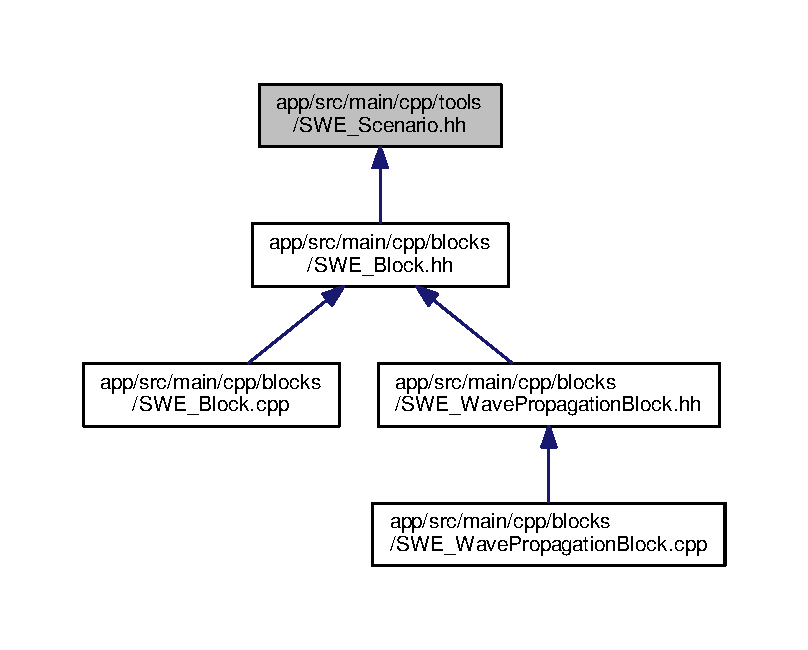
\includegraphics[width=350pt]{tools_2SWE__Scenario_8hh__dep__incl}
\end{center}
\end{figure}
\subsection*{Classes}
\begin{DoxyCompactItemize}
\item 
class \hyperlink{classSWE__Scenario}{S\+W\+E\+\_\+\+Scenario}
\begin{DoxyCompactList}\small\item\em This class sets the standart layout for all simulateable scenarios. \end{DoxyCompactList}\end{DoxyCompactItemize}
\subsection*{Typedefs}
\begin{DoxyCompactItemize}
\item 
typedef enum \hyperlink{scenarios_2SWE__Scenario_8hh_af75d5dd7322fa39ed0af4e7839e600f8}{Boundary\+Type} \hyperlink{tools_2SWE__Scenario_8hh_a0076a482278ddc13ed179c6c76c9b5ad}{Boundary\+Type}
\item 
typedef enum \hyperlink{scenarios_2SWE__Scenario_8hh_aa5e01e3f7df312f7b9b0d02521141fcc}{Boundary\+Edge} \hyperlink{tools_2SWE__Scenario_8hh_a53b43e70a19e542b4c1ab2da9c6bcc0e}{Boundary\+Edge}
\end{DoxyCompactItemize}
\subsection*{Enumerations}
\begin{DoxyCompactItemize}
\item 
enum \hyperlink{tools_2SWE__Scenario_8hh_af75d5dd7322fa39ed0af4e7839e600f8}{Boundary\+Type} \{ \\*
\hyperlink{scenarios_2SWE__Scenario_8hh_af75d5dd7322fa39ed0af4e7839e600f8abfcb976304836f3d329c3b7c8b7dbb63}{O\+U\+T\+F\+L\+OW}, 
\hyperlink{scenarios_2SWE__Scenario_8hh_af75d5dd7322fa39ed0af4e7839e600f8afca2faad41310c7e71ec303ef789c53a}{W\+A\+LL}, 
\hyperlink{scenarios_2SWE__Scenario_8hh_af75d5dd7322fa39ed0af4e7839e600f8a8c7e97da6bd5c3568ccc5ee6cd958c87}{I\+N\+F\+L\+OW}, 
\hyperlink{scenarios_2SWE__Scenario_8hh_af75d5dd7322fa39ed0af4e7839e600f8a20391dd2915a0e64343d24c2f2e40b95}{C\+O\+N\+N\+E\+CT}, 
\\*
\hyperlink{scenarios_2SWE__Scenario_8hh_af75d5dd7322fa39ed0af4e7839e600f8a48be352751e0dd34bbad624be5667ee2}{P\+A\+S\+S\+I\+VE}, 
\hyperlink{tools_2SWE__Scenario_8hh_af75d5dd7322fa39ed0af4e7839e600f8abfcb976304836f3d329c3b7c8b7dbb63}{O\+U\+T\+F\+L\+OW}, 
\hyperlink{tools_2SWE__Scenario_8hh_af75d5dd7322fa39ed0af4e7839e600f8afca2faad41310c7e71ec303ef789c53a}{W\+A\+LL}, 
\hyperlink{tools_2SWE__Scenario_8hh_af75d5dd7322fa39ed0af4e7839e600f8a8c7e97da6bd5c3568ccc5ee6cd958c87}{I\+N\+F\+L\+OW}, 
\\*
\hyperlink{tools_2SWE__Scenario_8hh_af75d5dd7322fa39ed0af4e7839e600f8a20391dd2915a0e64343d24c2f2e40b95}{C\+O\+N\+N\+E\+CT}, 
\hyperlink{tools_2SWE__Scenario_8hh_af75d5dd7322fa39ed0af4e7839e600f8a48be352751e0dd34bbad624be5667ee2}{P\+A\+S\+S\+I\+VE}
 \}
\item 
enum \hyperlink{tools_2SWE__Scenario_8hh_aa5e01e3f7df312f7b9b0d02521141fcc}{Boundary\+Edge} \{ \\*
\hyperlink{scenarios_2SWE__Scenario_8hh_aa5e01e3f7df312f7b9b0d02521141fcca34eeb3a076f3bbcb32d47b74ee3cee86}{B\+N\+D\+\_\+\+L\+E\+FT}, 
\hyperlink{scenarios_2SWE__Scenario_8hh_aa5e01e3f7df312f7b9b0d02521141fccac0391ea6a5bf43f7735142e9ae87a62f}{B\+N\+D\+\_\+\+R\+I\+G\+HT}, 
\hyperlink{scenarios_2SWE__Scenario_8hh_aa5e01e3f7df312f7b9b0d02521141fccaff0478ddcbdcce0a6af3a9dc75445380}{B\+N\+D\+\_\+\+B\+O\+T\+T\+OM}, 
\hyperlink{scenarios_2SWE__Scenario_8hh_aa5e01e3f7df312f7b9b0d02521141fcca80c82ce939775733d407d69e30f74177}{B\+N\+D\+\_\+\+T\+OP}, 
\\*
\hyperlink{tools_2SWE__Scenario_8hh_aa5e01e3f7df312f7b9b0d02521141fcca34eeb3a076f3bbcb32d47b74ee3cee86}{B\+N\+D\+\_\+\+L\+E\+FT}, 
\hyperlink{tools_2SWE__Scenario_8hh_aa5e01e3f7df312f7b9b0d02521141fccac0391ea6a5bf43f7735142e9ae87a62f}{B\+N\+D\+\_\+\+R\+I\+G\+HT}, 
\hyperlink{tools_2SWE__Scenario_8hh_aa5e01e3f7df312f7b9b0d02521141fccaff0478ddcbdcce0a6af3a9dc75445380}{B\+N\+D\+\_\+\+B\+O\+T\+T\+OM}, 
\hyperlink{tools_2SWE__Scenario_8hh_aa5e01e3f7df312f7b9b0d02521141fcca80c82ce939775733d407d69e30f74177}{B\+N\+D\+\_\+\+T\+OP}
 \}
\end{DoxyCompactItemize}


\subsection{Typedef Documentation}
\index{tools/\+S\+W\+E\+\_\+\+Scenario.\+hh@{tools/\+S\+W\+E\+\_\+\+Scenario.\+hh}!Boundary\+Edge@{Boundary\+Edge}}
\index{Boundary\+Edge@{Boundary\+Edge}!tools/\+S\+W\+E\+\_\+\+Scenario.\+hh@{tools/\+S\+W\+E\+\_\+\+Scenario.\+hh}}
\subsubsection[{\texorpdfstring{Boundary\+Edge}{BoundaryEdge}}]{\setlength{\rightskip}{0pt plus 5cm}typedef enum {\bf Boundary\+Edge}  {\bf Boundary\+Edge}}\hypertarget{tools_2SWE__Scenario_8hh_a53b43e70a19e542b4c1ab2da9c6bcc0e}{}\label{tools_2SWE__Scenario_8hh_a53b43e70a19e542b4c1ab2da9c6bcc0e}
enum type\+: numbering of the boundary edges \index{tools/\+S\+W\+E\+\_\+\+Scenario.\+hh@{tools/\+S\+W\+E\+\_\+\+Scenario.\+hh}!Boundary\+Type@{Boundary\+Type}}
\index{Boundary\+Type@{Boundary\+Type}!tools/\+S\+W\+E\+\_\+\+Scenario.\+hh@{tools/\+S\+W\+E\+\_\+\+Scenario.\+hh}}
\subsubsection[{\texorpdfstring{Boundary\+Type}{BoundaryType}}]{\setlength{\rightskip}{0pt plus 5cm}typedef enum {\bf Boundary\+Type}  {\bf Boundary\+Type}}\hypertarget{tools_2SWE__Scenario_8hh_a0076a482278ddc13ed179c6c76c9b5ad}{}\label{tools_2SWE__Scenario_8hh_a0076a482278ddc13ed179c6c76c9b5ad}
enum type\+: available types of boundary conditions 

\subsection{Enumeration Type Documentation}
\index{tools/\+S\+W\+E\+\_\+\+Scenario.\+hh@{tools/\+S\+W\+E\+\_\+\+Scenario.\+hh}!Boundary\+Edge@{Boundary\+Edge}}
\index{Boundary\+Edge@{Boundary\+Edge}!tools/\+S\+W\+E\+\_\+\+Scenario.\+hh@{tools/\+S\+W\+E\+\_\+\+Scenario.\+hh}}
\subsubsection[{\texorpdfstring{Boundary\+Edge}{BoundaryEdge}}]{\setlength{\rightskip}{0pt plus 5cm}enum {\bf Boundary\+Edge}}\hypertarget{tools_2SWE__Scenario_8hh_aa5e01e3f7df312f7b9b0d02521141fcc}{}\label{tools_2SWE__Scenario_8hh_aa5e01e3f7df312f7b9b0d02521141fcc}
enum type\+: numbering of the boundary edges \begin{Desc}
\item[Enumerator]\par
\begin{description}
\index{B\+N\+D\+\_\+\+L\+E\+FT@{B\+N\+D\+\_\+\+L\+E\+FT}!tools/\+S\+W\+E\+\_\+\+Scenario.\+hh@{tools/\+S\+W\+E\+\_\+\+Scenario.\+hh}}\index{tools/\+S\+W\+E\+\_\+\+Scenario.\+hh@{tools/\+S\+W\+E\+\_\+\+Scenario.\+hh}!B\+N\+D\+\_\+\+L\+E\+FT@{B\+N\+D\+\_\+\+L\+E\+FT}}\item[{\em 
B\+N\+D\+\_\+\+L\+E\+FT\hypertarget{tools_2SWE__Scenario_8hh_aa5e01e3f7df312f7b9b0d02521141fcca34eeb3a076f3bbcb32d47b74ee3cee86}{}\label{tools_2SWE__Scenario_8hh_aa5e01e3f7df312f7b9b0d02521141fcca34eeb3a076f3bbcb32d47b74ee3cee86}
}]\index{B\+N\+D\+\_\+\+R\+I\+G\+HT@{B\+N\+D\+\_\+\+R\+I\+G\+HT}!tools/\+S\+W\+E\+\_\+\+Scenario.\+hh@{tools/\+S\+W\+E\+\_\+\+Scenario.\+hh}}\index{tools/\+S\+W\+E\+\_\+\+Scenario.\+hh@{tools/\+S\+W\+E\+\_\+\+Scenario.\+hh}!B\+N\+D\+\_\+\+R\+I\+G\+HT@{B\+N\+D\+\_\+\+R\+I\+G\+HT}}\item[{\em 
B\+N\+D\+\_\+\+R\+I\+G\+HT\hypertarget{tools_2SWE__Scenario_8hh_aa5e01e3f7df312f7b9b0d02521141fccac0391ea6a5bf43f7735142e9ae87a62f}{}\label{tools_2SWE__Scenario_8hh_aa5e01e3f7df312f7b9b0d02521141fccac0391ea6a5bf43f7735142e9ae87a62f}
}]\index{B\+N\+D\+\_\+\+B\+O\+T\+T\+OM@{B\+N\+D\+\_\+\+B\+O\+T\+T\+OM}!tools/\+S\+W\+E\+\_\+\+Scenario.\+hh@{tools/\+S\+W\+E\+\_\+\+Scenario.\+hh}}\index{tools/\+S\+W\+E\+\_\+\+Scenario.\+hh@{tools/\+S\+W\+E\+\_\+\+Scenario.\+hh}!B\+N\+D\+\_\+\+B\+O\+T\+T\+OM@{B\+N\+D\+\_\+\+B\+O\+T\+T\+OM}}\item[{\em 
B\+N\+D\+\_\+\+B\+O\+T\+T\+OM\hypertarget{tools_2SWE__Scenario_8hh_aa5e01e3f7df312f7b9b0d02521141fccaff0478ddcbdcce0a6af3a9dc75445380}{}\label{tools_2SWE__Scenario_8hh_aa5e01e3f7df312f7b9b0d02521141fccaff0478ddcbdcce0a6af3a9dc75445380}
}]\index{B\+N\+D\+\_\+\+T\+OP@{B\+N\+D\+\_\+\+T\+OP}!tools/\+S\+W\+E\+\_\+\+Scenario.\+hh@{tools/\+S\+W\+E\+\_\+\+Scenario.\+hh}}\index{tools/\+S\+W\+E\+\_\+\+Scenario.\+hh@{tools/\+S\+W\+E\+\_\+\+Scenario.\+hh}!B\+N\+D\+\_\+\+T\+OP@{B\+N\+D\+\_\+\+T\+OP}}\item[{\em 
B\+N\+D\+\_\+\+T\+OP\hypertarget{tools_2SWE__Scenario_8hh_aa5e01e3f7df312f7b9b0d02521141fcca80c82ce939775733d407d69e30f74177}{}\label{tools_2SWE__Scenario_8hh_aa5e01e3f7df312f7b9b0d02521141fcca80c82ce939775733d407d69e30f74177}
}]\index{B\+N\+D\+\_\+\+L\+E\+FT@{B\+N\+D\+\_\+\+L\+E\+FT}!tools/\+S\+W\+E\+\_\+\+Scenario.\+hh@{tools/\+S\+W\+E\+\_\+\+Scenario.\+hh}}\index{tools/\+S\+W\+E\+\_\+\+Scenario.\+hh@{tools/\+S\+W\+E\+\_\+\+Scenario.\+hh}!B\+N\+D\+\_\+\+L\+E\+FT@{B\+N\+D\+\_\+\+L\+E\+FT}}\item[{\em 
B\+N\+D\+\_\+\+L\+E\+FT\hypertarget{tools_2SWE__Scenario_8hh_aa5e01e3f7df312f7b9b0d02521141fcca34eeb3a076f3bbcb32d47b74ee3cee86}{}\label{tools_2SWE__Scenario_8hh_aa5e01e3f7df312f7b9b0d02521141fcca34eeb3a076f3bbcb32d47b74ee3cee86}
}]\index{B\+N\+D\+\_\+\+R\+I\+G\+HT@{B\+N\+D\+\_\+\+R\+I\+G\+HT}!tools/\+S\+W\+E\+\_\+\+Scenario.\+hh@{tools/\+S\+W\+E\+\_\+\+Scenario.\+hh}}\index{tools/\+S\+W\+E\+\_\+\+Scenario.\+hh@{tools/\+S\+W\+E\+\_\+\+Scenario.\+hh}!B\+N\+D\+\_\+\+R\+I\+G\+HT@{B\+N\+D\+\_\+\+R\+I\+G\+HT}}\item[{\em 
B\+N\+D\+\_\+\+R\+I\+G\+HT\hypertarget{tools_2SWE__Scenario_8hh_aa5e01e3f7df312f7b9b0d02521141fccac0391ea6a5bf43f7735142e9ae87a62f}{}\label{tools_2SWE__Scenario_8hh_aa5e01e3f7df312f7b9b0d02521141fccac0391ea6a5bf43f7735142e9ae87a62f}
}]\index{B\+N\+D\+\_\+\+B\+O\+T\+T\+OM@{B\+N\+D\+\_\+\+B\+O\+T\+T\+OM}!tools/\+S\+W\+E\+\_\+\+Scenario.\+hh@{tools/\+S\+W\+E\+\_\+\+Scenario.\+hh}}\index{tools/\+S\+W\+E\+\_\+\+Scenario.\+hh@{tools/\+S\+W\+E\+\_\+\+Scenario.\+hh}!B\+N\+D\+\_\+\+B\+O\+T\+T\+OM@{B\+N\+D\+\_\+\+B\+O\+T\+T\+OM}}\item[{\em 
B\+N\+D\+\_\+\+B\+O\+T\+T\+OM\hypertarget{tools_2SWE__Scenario_8hh_aa5e01e3f7df312f7b9b0d02521141fccaff0478ddcbdcce0a6af3a9dc75445380}{}\label{tools_2SWE__Scenario_8hh_aa5e01e3f7df312f7b9b0d02521141fccaff0478ddcbdcce0a6af3a9dc75445380}
}]\index{B\+N\+D\+\_\+\+T\+OP@{B\+N\+D\+\_\+\+T\+OP}!tools/\+S\+W\+E\+\_\+\+Scenario.\+hh@{tools/\+S\+W\+E\+\_\+\+Scenario.\+hh}}\index{tools/\+S\+W\+E\+\_\+\+Scenario.\+hh@{tools/\+S\+W\+E\+\_\+\+Scenario.\+hh}!B\+N\+D\+\_\+\+T\+OP@{B\+N\+D\+\_\+\+T\+OP}}\item[{\em 
B\+N\+D\+\_\+\+T\+OP\hypertarget{tools_2SWE__Scenario_8hh_aa5e01e3f7df312f7b9b0d02521141fcca80c82ce939775733d407d69e30f74177}{}\label{tools_2SWE__Scenario_8hh_aa5e01e3f7df312f7b9b0d02521141fcca80c82ce939775733d407d69e30f74177}
}]\end{description}
\end{Desc}


Definition at line 41 of file S\+W\+E\+\_\+\+Scenario.\+hh.

\index{tools/\+S\+W\+E\+\_\+\+Scenario.\+hh@{tools/\+S\+W\+E\+\_\+\+Scenario.\+hh}!Boundary\+Type@{Boundary\+Type}}
\index{Boundary\+Type@{Boundary\+Type}!tools/\+S\+W\+E\+\_\+\+Scenario.\+hh@{tools/\+S\+W\+E\+\_\+\+Scenario.\+hh}}
\subsubsection[{\texorpdfstring{Boundary\+Type}{BoundaryType}}]{\setlength{\rightskip}{0pt plus 5cm}enum {\bf Boundary\+Type}}\hypertarget{tools_2SWE__Scenario_8hh_af75d5dd7322fa39ed0af4e7839e600f8}{}\label{tools_2SWE__Scenario_8hh_af75d5dd7322fa39ed0af4e7839e600f8}
enum type\+: available types of boundary conditions \begin{Desc}
\item[Enumerator]\par
\begin{description}
\index{O\+U\+T\+F\+L\+OW@{O\+U\+T\+F\+L\+OW}!tools/\+S\+W\+E\+\_\+\+Scenario.\+hh@{tools/\+S\+W\+E\+\_\+\+Scenario.\+hh}}\index{tools/\+S\+W\+E\+\_\+\+Scenario.\+hh@{tools/\+S\+W\+E\+\_\+\+Scenario.\+hh}!O\+U\+T\+F\+L\+OW@{O\+U\+T\+F\+L\+OW}}\item[{\em 
O\+U\+T\+F\+L\+OW\hypertarget{tools_2SWE__Scenario_8hh_af75d5dd7322fa39ed0af4e7839e600f8abfcb976304836f3d329c3b7c8b7dbb63}{}\label{tools_2SWE__Scenario_8hh_af75d5dd7322fa39ed0af4e7839e600f8abfcb976304836f3d329c3b7c8b7dbb63}
}]\index{W\+A\+LL@{W\+A\+LL}!tools/\+S\+W\+E\+\_\+\+Scenario.\+hh@{tools/\+S\+W\+E\+\_\+\+Scenario.\+hh}}\index{tools/\+S\+W\+E\+\_\+\+Scenario.\+hh@{tools/\+S\+W\+E\+\_\+\+Scenario.\+hh}!W\+A\+LL@{W\+A\+LL}}\item[{\em 
W\+A\+LL\hypertarget{tools_2SWE__Scenario_8hh_af75d5dd7322fa39ed0af4e7839e600f8afca2faad41310c7e71ec303ef789c53a}{}\label{tools_2SWE__Scenario_8hh_af75d5dd7322fa39ed0af4e7839e600f8afca2faad41310c7e71ec303ef789c53a}
}]\index{I\+N\+F\+L\+OW@{I\+N\+F\+L\+OW}!tools/\+S\+W\+E\+\_\+\+Scenario.\+hh@{tools/\+S\+W\+E\+\_\+\+Scenario.\+hh}}\index{tools/\+S\+W\+E\+\_\+\+Scenario.\+hh@{tools/\+S\+W\+E\+\_\+\+Scenario.\+hh}!I\+N\+F\+L\+OW@{I\+N\+F\+L\+OW}}\item[{\em 
I\+N\+F\+L\+OW\hypertarget{tools_2SWE__Scenario_8hh_af75d5dd7322fa39ed0af4e7839e600f8a8c7e97da6bd5c3568ccc5ee6cd958c87}{}\label{tools_2SWE__Scenario_8hh_af75d5dd7322fa39ed0af4e7839e600f8a8c7e97da6bd5c3568ccc5ee6cd958c87}
}]\index{C\+O\+N\+N\+E\+CT@{C\+O\+N\+N\+E\+CT}!tools/\+S\+W\+E\+\_\+\+Scenario.\+hh@{tools/\+S\+W\+E\+\_\+\+Scenario.\+hh}}\index{tools/\+S\+W\+E\+\_\+\+Scenario.\+hh@{tools/\+S\+W\+E\+\_\+\+Scenario.\+hh}!C\+O\+N\+N\+E\+CT@{C\+O\+N\+N\+E\+CT}}\item[{\em 
C\+O\+N\+N\+E\+CT\hypertarget{tools_2SWE__Scenario_8hh_af75d5dd7322fa39ed0af4e7839e600f8a20391dd2915a0e64343d24c2f2e40b95}{}\label{tools_2SWE__Scenario_8hh_af75d5dd7322fa39ed0af4e7839e600f8a20391dd2915a0e64343d24c2f2e40b95}
}]\index{P\+A\+S\+S\+I\+VE@{P\+A\+S\+S\+I\+VE}!tools/\+S\+W\+E\+\_\+\+Scenario.\+hh@{tools/\+S\+W\+E\+\_\+\+Scenario.\+hh}}\index{tools/\+S\+W\+E\+\_\+\+Scenario.\+hh@{tools/\+S\+W\+E\+\_\+\+Scenario.\+hh}!P\+A\+S\+S\+I\+VE@{P\+A\+S\+S\+I\+VE}}\item[{\em 
P\+A\+S\+S\+I\+VE\hypertarget{tools_2SWE__Scenario_8hh_af75d5dd7322fa39ed0af4e7839e600f8a48be352751e0dd34bbad624be5667ee2}{}\label{tools_2SWE__Scenario_8hh_af75d5dd7322fa39ed0af4e7839e600f8a48be352751e0dd34bbad624be5667ee2}
}]\index{O\+U\+T\+F\+L\+OW@{O\+U\+T\+F\+L\+OW}!tools/\+S\+W\+E\+\_\+\+Scenario.\+hh@{tools/\+S\+W\+E\+\_\+\+Scenario.\+hh}}\index{tools/\+S\+W\+E\+\_\+\+Scenario.\+hh@{tools/\+S\+W\+E\+\_\+\+Scenario.\+hh}!O\+U\+T\+F\+L\+OW@{O\+U\+T\+F\+L\+OW}}\item[{\em 
O\+U\+T\+F\+L\+OW\hypertarget{tools_2SWE__Scenario_8hh_af75d5dd7322fa39ed0af4e7839e600f8abfcb976304836f3d329c3b7c8b7dbb63}{}\label{tools_2SWE__Scenario_8hh_af75d5dd7322fa39ed0af4e7839e600f8abfcb976304836f3d329c3b7c8b7dbb63}
}]\index{W\+A\+LL@{W\+A\+LL}!tools/\+S\+W\+E\+\_\+\+Scenario.\+hh@{tools/\+S\+W\+E\+\_\+\+Scenario.\+hh}}\index{tools/\+S\+W\+E\+\_\+\+Scenario.\+hh@{tools/\+S\+W\+E\+\_\+\+Scenario.\+hh}!W\+A\+LL@{W\+A\+LL}}\item[{\em 
W\+A\+LL\hypertarget{tools_2SWE__Scenario_8hh_af75d5dd7322fa39ed0af4e7839e600f8afca2faad41310c7e71ec303ef789c53a}{}\label{tools_2SWE__Scenario_8hh_af75d5dd7322fa39ed0af4e7839e600f8afca2faad41310c7e71ec303ef789c53a}
}]\index{I\+N\+F\+L\+OW@{I\+N\+F\+L\+OW}!tools/\+S\+W\+E\+\_\+\+Scenario.\+hh@{tools/\+S\+W\+E\+\_\+\+Scenario.\+hh}}\index{tools/\+S\+W\+E\+\_\+\+Scenario.\+hh@{tools/\+S\+W\+E\+\_\+\+Scenario.\+hh}!I\+N\+F\+L\+OW@{I\+N\+F\+L\+OW}}\item[{\em 
I\+N\+F\+L\+OW\hypertarget{tools_2SWE__Scenario_8hh_af75d5dd7322fa39ed0af4e7839e600f8a8c7e97da6bd5c3568ccc5ee6cd958c87}{}\label{tools_2SWE__Scenario_8hh_af75d5dd7322fa39ed0af4e7839e600f8a8c7e97da6bd5c3568ccc5ee6cd958c87}
}]\index{C\+O\+N\+N\+E\+CT@{C\+O\+N\+N\+E\+CT}!tools/\+S\+W\+E\+\_\+\+Scenario.\+hh@{tools/\+S\+W\+E\+\_\+\+Scenario.\+hh}}\index{tools/\+S\+W\+E\+\_\+\+Scenario.\+hh@{tools/\+S\+W\+E\+\_\+\+Scenario.\+hh}!C\+O\+N\+N\+E\+CT@{C\+O\+N\+N\+E\+CT}}\item[{\em 
C\+O\+N\+N\+E\+CT\hypertarget{tools_2SWE__Scenario_8hh_af75d5dd7322fa39ed0af4e7839e600f8a20391dd2915a0e64343d24c2f2e40b95}{}\label{tools_2SWE__Scenario_8hh_af75d5dd7322fa39ed0af4e7839e600f8a20391dd2915a0e64343d24c2f2e40b95}
}]\index{P\+A\+S\+S\+I\+VE@{P\+A\+S\+S\+I\+VE}!tools/\+S\+W\+E\+\_\+\+Scenario.\+hh@{tools/\+S\+W\+E\+\_\+\+Scenario.\+hh}}\index{tools/\+S\+W\+E\+\_\+\+Scenario.\+hh@{tools/\+S\+W\+E\+\_\+\+Scenario.\+hh}!P\+A\+S\+S\+I\+VE@{P\+A\+S\+S\+I\+VE}}\item[{\em 
P\+A\+S\+S\+I\+VE\hypertarget{tools_2SWE__Scenario_8hh_af75d5dd7322fa39ed0af4e7839e600f8a48be352751e0dd34bbad624be5667ee2}{}\label{tools_2SWE__Scenario_8hh_af75d5dd7322fa39ed0af4e7839e600f8a48be352751e0dd34bbad624be5667ee2}
}]\end{description}
\end{Desc}


Definition at line 34 of file S\+W\+E\+\_\+\+Scenario.\+hh.


\hypertarget{SWE__simple__scenarios_8hh}{}\section{app/src/main/cpp/scenarios/\+S\+W\+E\+\_\+simple\+\_\+scenarios.hh File Reference}
\label{SWE__simple__scenarios_8hh}\index{app/src/main/cpp/scenarios/\+S\+W\+E\+\_\+simple\+\_\+scenarios.\+hh@{app/src/main/cpp/scenarios/\+S\+W\+E\+\_\+simple\+\_\+scenarios.\+hh}}
{\ttfamily \#include $<$cmath$>$}\\*
{\ttfamily \#include \char`\"{}../tools/help.\+hh\char`\"{}}\\*
{\ttfamily \#include \char`\"{}S\+W\+E\+\_\+\+Scenario.\+hh\char`\"{}}\\*
Include dependency graph for S\+W\+E\+\_\+simple\+\_\+scenarios.\+hh\+:\nopagebreak
\begin{figure}[H]
\begin{center}
\leavevmode
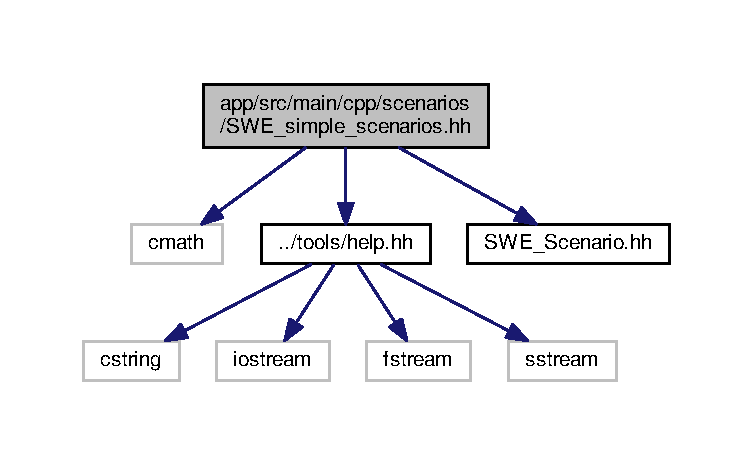
\includegraphics[width=350pt]{SWE__simple__scenarios_8hh__incl}
\end{center}
\end{figure}
\subsection*{Classes}
\begin{DoxyCompactItemize}
\item 
class \hyperlink{classSWE__RadialDamBreakScenario}{S\+W\+E\+\_\+\+Radial\+Dam\+Break\+Scenario}
\begin{DoxyCompactList}\small\item\em scenario is a test environment for the apps later wave-\/positioninig and its influence on the surrounding sea \end{DoxyCompactList}\end{DoxyCompactItemize}


\subsection{Detailed Description}
This file is part of S\+WE.

\begin{DoxyAuthor}{Author}
Michael Bader, Kaveh Rahnema, Tobias Schnabel 

Sebastian Rettenberger (rettenbs AT in.\+tum.\+de, \href{http://www5.in.tum.de/wiki/index.php/Sebastian_Rettenberger,_M.Sc}{\tt http\+://www5.\+in.\+tum.\+de/wiki/index.\+php/\+Sebastian\+\_\+\+Rettenberger,\+\_\+\+M.\+Sc}.)
\end{DoxyAuthor}
\hypertarget{help_8hh_LICENSE}{}\subsection{L\+I\+C\+E\+N\+SE}\label{help_8hh_LICENSE}
S\+WE is free software\+: you can redistribute it and/or modify it under the terms of the G\+NU General Public License as published by the Free Software Foundation, either version 3 of the License, or (at your option) any later version.

S\+WE is distributed in the hope that it will be useful, but W\+I\+T\+H\+O\+UT A\+NY W\+A\+R\+R\+A\+N\+TY; without even the implied warranty of M\+E\+R\+C\+H\+A\+N\+T\+A\+B\+I\+L\+I\+TY or F\+I\+T\+N\+E\+SS F\+OR A P\+A\+R\+T\+I\+C\+U\+L\+AR P\+U\+R\+P\+O\+SE. See the G\+NU General Public License for more details.

You should have received a copy of the G\+NU General Public License along with S\+WE. If not, see \href{http://www.gnu.org/licenses/}{\tt http\+://www.\+gnu.\+org/licenses/}.\hypertarget{help_8hh_DESCRIPTION}{}\subsection{D\+E\+S\+C\+R\+I\+P\+T\+I\+ON}\label{help_8hh_DESCRIPTION}
T\+O\+DO 
\hypertarget{help_8hh}{}\section{app/src/main/cpp/tools/help.hh File Reference}
\label{help_8hh}\index{app/src/main/cpp/tools/help.\+hh@{app/src/main/cpp/tools/help.\+hh}}
{\ttfamily \#include $<$cstring$>$}\\*
{\ttfamily \#include $<$iostream$>$}\\*
{\ttfamily \#include $<$fstream$>$}\\*
{\ttfamily \#include $<$sstream$>$}\\*
Include dependency graph for help.\+hh\+:\nopagebreak
\begin{figure}[H]
\begin{center}
\leavevmode
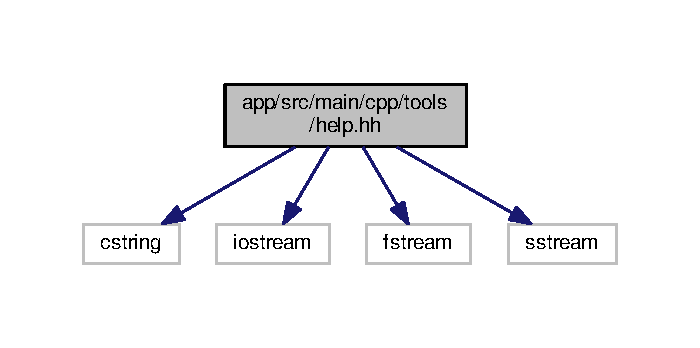
\includegraphics[width=336pt]{help_8hh__incl}
\end{center}
\end{figure}
This graph shows which files directly or indirectly include this file\+:\nopagebreak
\begin{figure}[H]
\begin{center}
\leavevmode
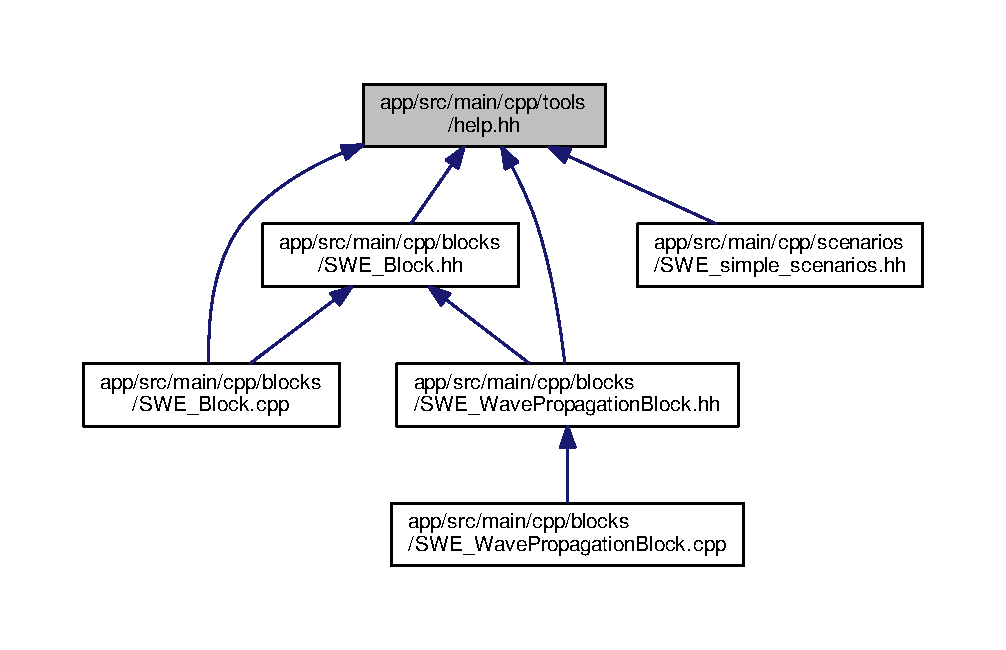
\includegraphics[width=350pt]{help_8hh__dep__incl}
\end{center}
\end{figure}
\subsection*{Classes}
\begin{DoxyCompactItemize}
\item 
class \hyperlink{classFloat1D}{Float1D}
\begin{DoxyCompactList}\small\item\em This class is part of S\+WE; It gives our representation of a one dimensional datatype for update calculations. \end{DoxyCompactList}\item 
class \hyperlink{classFloat2D}{Float2D}
\begin{DoxyCompactList}\small\item\em This class is part of S\+WE; It gives our representation of atwo dimensional datatype for update calculations. \end{DoxyCompactList}\end{DoxyCompactItemize}
\subsection*{Functions}
\begin{DoxyCompactItemize}
\item 
std\+::string \hyperlink{help_8hh_aa10dc278c6ac60f9cd49955cbe16fbcb}{generate\+File\+Name} (std\+::string base\+Name, int time\+Step)
\item 
std\+::string \hyperlink{help_8hh_a206f33ce37fa47f8635d02a1cfc9881f}{generate\+File\+Name} (std\+::string i\+\_\+base\+Name, int i\+\_\+block\+PositionX, int i\+\_\+block\+PositionY, std\+::string i\+\_\+file\+Extension=\char`\"{}.nc\char`\"{})
\item 
std\+::string \hyperlink{help_8hh_ab05bce4e4d30d0b9fb85f81668f98f79}{generate\+File\+Name} (std\+::string base\+Name, int time\+Step, int block\+\_\+X, int block\+\_\+Y, std\+::string i\+\_\+file\+Extension=\char`\"{}.vts\char`\"{})
\item 
std\+::string \hyperlink{help_8hh_a7dc37444a6b7771aefff04a38e74e086}{generate\+Base\+File\+Name} (std\+::string \&i\+\_\+base\+Name, int i\+\_\+block\+PositionX, int i\+\_\+block\+PositionY)
\item 
std\+::string \hyperlink{help_8hh_a427928180ec14bf889c55e5cc51d8e36}{generate\+Container\+File\+Name} (std\+::string base\+Name, int time\+Step)
\end{DoxyCompactItemize}


\subsection{Detailed Description}
This file is part of S\+WE.

\begin{DoxyAuthor}{Author}
Michael Bader, Kaveh Rahnema 

Sebastian Rettenberger
\end{DoxyAuthor}
\hypertarget{help_8hh_LICENSE}{}\subsection{L\+I\+C\+E\+N\+SE}\label{help_8hh_LICENSE}
S\+WE is free software\+: you can redistribute it and/or modify it under the terms of the G\+NU General Public License as published by the Free Software Foundation, either version 3 of the License, or (at your option) any later version.

S\+WE is distributed in the hope that it will be useful, but W\+I\+T\+H\+O\+UT A\+NY W\+A\+R\+R\+A\+N\+TY; without even the implied warranty of M\+E\+R\+C\+H\+A\+N\+T\+A\+B\+I\+L\+I\+TY or F\+I\+T\+N\+E\+SS F\+OR A P\+A\+R\+T\+I\+C\+U\+L\+AR P\+U\+R\+P\+O\+SE. See the G\+NU General Public License for more details.

You should have received a copy of the G\+NU General Public License along with S\+WE. If not, see \href{http://www.gnu.org/licenses/}{\tt http\+://www.\+gnu.\+org/licenses/}.\hypertarget{help_8hh_DESCRIPTION}{}\subsection{D\+E\+S\+C\+R\+I\+P\+T\+I\+ON}\label{help_8hh_DESCRIPTION}
T\+O\+DO 

\subsection{Function Documentation}
\index{help.\+hh@{help.\+hh}!generate\+Base\+File\+Name@{generate\+Base\+File\+Name}}
\index{generate\+Base\+File\+Name@{generate\+Base\+File\+Name}!help.\+hh@{help.\+hh}}
\subsubsection[{\texorpdfstring{generate\+Base\+File\+Name(std\+::string \&i\+\_\+base\+Name, int i\+\_\+block\+Position\+X, int i\+\_\+block\+Position\+Y)}{generateBaseFileName(std::string &i_baseName, int i_blockPositionX, int i_blockPositionY)}}]{\setlength{\rightskip}{0pt plus 5cm}std\+::string generate\+Base\+File\+Name (
\begin{DoxyParamCaption}
\item[{std\+::string \&}]{i\+\_\+base\+Name, }
\item[{int}]{i\+\_\+block\+PositionX, }
\item[{int}]{i\+\_\+block\+PositionY}
\end{DoxyParamCaption}
)\hspace{0.3cm}{\ttfamily [inline]}}\hypertarget{help_8hh_a7dc37444a6b7771aefff04a38e74e086}{}\label{help_8hh_a7dc37444a6b7771aefff04a38e74e086}
Generates an output file name for a multiple \hyperlink{classSWE__Block}{S\+W\+E\+\_\+\+Block} version based on the ordering of the blocks.


\begin{DoxyParams}{Parameters}
{\em i\+\_\+base\+Name} & base name of the output. \\
\hline
{\em i\+\_\+block\+PositionX} & position of the \hyperlink{classSWE__Block}{S\+W\+E\+\_\+\+Block} in x-\/direction. \\
\hline
{\em i\+\_\+block\+PositionY} & position of the \hyperlink{classSWE__Block}{S\+W\+E\+\_\+\+Block} in y-\/direction.\\
\hline
\end{DoxyParams}
\begin{DoxyReturn}{Returns}
the output filename {\bfseries without} timestep information and file extension 
\end{DoxyReturn}


Definition at line 253 of file help.\+hh.

\index{help.\+hh@{help.\+hh}!generate\+Container\+File\+Name@{generate\+Container\+File\+Name}}
\index{generate\+Container\+File\+Name@{generate\+Container\+File\+Name}!help.\+hh@{help.\+hh}}
\subsubsection[{\texorpdfstring{generate\+Container\+File\+Name(std\+::string base\+Name, int time\+Step)}{generateContainerFileName(std::string baseName, int timeStep)}}]{\setlength{\rightskip}{0pt plus 5cm}std\+::string generate\+Container\+File\+Name (
\begin{DoxyParamCaption}
\item[{std\+::string}]{base\+Name, }
\item[{int}]{time\+Step}
\end{DoxyParamCaption}
)\hspace{0.3cm}{\ttfamily [inline]}}\hypertarget{help_8hh_a427928180ec14bf889c55e5cc51d8e36}{}\label{help_8hh_a427928180ec14bf889c55e5cc51d8e36}
generate output filename for the Para\+View-\/\+Container-\/\+File (to visualize multiple S\+W\+E\+\_\+\+Blocks per checkpoint) 

Definition at line 265 of file help.\+hh.

\index{help.\+hh@{help.\+hh}!generate\+File\+Name@{generate\+File\+Name}}
\index{generate\+File\+Name@{generate\+File\+Name}!help.\+hh@{help.\+hh}}
\subsubsection[{\texorpdfstring{generate\+File\+Name(std\+::string base\+Name, int time\+Step)}{generateFileName(std::string baseName, int timeStep)}}]{\setlength{\rightskip}{0pt plus 5cm}std\+::string generate\+File\+Name (
\begin{DoxyParamCaption}
\item[{std\+::string}]{base\+Name, }
\item[{int}]{time\+Step}
\end{DoxyParamCaption}
)\hspace{0.3cm}{\ttfamily [inline]}}\hypertarget{help_8hh_aa10dc278c6ac60f9cd49955cbe16fbcb}{}\label{help_8hh_aa10dc278c6ac60f9cd49955cbe16fbcb}
generate output filenames for the single-\/\+S\+W\+E\+\_\+\+Block version (for serial and Open\+M\+P-\/parallelised versions that use only a single \hyperlink{classSWE__Block}{S\+W\+E\+\_\+\+Block} -\/ one output file is generated per checkpoint)

\begin{DoxyRefDesc}{Deprecated}
\item[\hyperlink{deprecated__deprecated000001}{Deprecated}]\end{DoxyRefDesc}


Definition at line 200 of file help.\+hh.

\index{help.\+hh@{help.\+hh}!generate\+File\+Name@{generate\+File\+Name}}
\index{generate\+File\+Name@{generate\+File\+Name}!help.\+hh@{help.\+hh}}
\subsubsection[{\texorpdfstring{generate\+File\+Name(std\+::string i\+\_\+base\+Name, int i\+\_\+block\+Position\+X, int i\+\_\+block\+Position\+Y, std\+::string i\+\_\+file\+Extension="".\+nc"")}{generateFileName(std::string i_baseName, int i_blockPositionX, int i_blockPositionY, std::string i_fileExtension=".nc")}}]{\setlength{\rightskip}{0pt plus 5cm}std\+::string generate\+File\+Name (
\begin{DoxyParamCaption}
\item[{std\+::string}]{i\+\_\+base\+Name, }
\item[{int}]{i\+\_\+block\+PositionX, }
\item[{int}]{i\+\_\+block\+PositionY, }
\item[{std\+::string}]{i\+\_\+file\+Extension = {\ttfamily \char`\"{}.nc\char`\"{}}}
\end{DoxyParamCaption}
)\hspace{0.3cm}{\ttfamily [inline]}}\hypertarget{help_8hh_a206f33ce37fa47f8635d02a1cfc9881f}{}\label{help_8hh_a206f33ce37fa47f8635d02a1cfc9881f}
Generates an output file name for a multiple \hyperlink{classSWE__Block}{S\+W\+E\+\_\+\+Block} version based on the ordering of the blocks.


\begin{DoxyParams}{Parameters}
{\em i\+\_\+base\+Name} & base name of the output. \\
\hline
{\em i\+\_\+block\+PositionX} & position of the \hyperlink{classSWE__Block}{S\+W\+E\+\_\+\+Block} in x-\/direction. \\
\hline
{\em i\+\_\+block\+PositionY} & position of the \hyperlink{classSWE__Block}{S\+W\+E\+\_\+\+Block} in y-\/direction. \\
\hline
{\em i\+\_\+file\+Extension} & file extension of the output file. \\
\hline
\end{DoxyParams}
\begin{DoxyReturn}{Returns}

\end{DoxyReturn}
\begin{DoxyRefDesc}{Deprecated}
\item[\hyperlink{deprecated__deprecated000002}{Deprecated}]\end{DoxyRefDesc}


Definition at line 218 of file help.\+hh.

\index{help.\+hh@{help.\+hh}!generate\+File\+Name@{generate\+File\+Name}}
\index{generate\+File\+Name@{generate\+File\+Name}!help.\+hh@{help.\+hh}}
\subsubsection[{\texorpdfstring{generate\+File\+Name(std\+::string base\+Name, int time\+Step, int block\+\_\+\+X, int block\+\_\+\+Y, std\+::string i\+\_\+file\+Extension="".\+vts"")}{generateFileName(std::string baseName, int timeStep, int block_X, int block_Y, std::string i_fileExtension=".vts")}}]{\setlength{\rightskip}{0pt plus 5cm}std\+::string generate\+File\+Name (
\begin{DoxyParamCaption}
\item[{std\+::string}]{base\+Name, }
\item[{int}]{time\+Step, }
\item[{int}]{block\+\_\+X, }
\item[{int}]{block\+\_\+Y, }
\item[{std\+::string}]{i\+\_\+file\+Extension = {\ttfamily \char`\"{}.vts\char`\"{}}}
\end{DoxyParamCaption}
)\hspace{0.3cm}{\ttfamily [inline]}}\hypertarget{help_8hh_ab05bce4e4d30d0b9fb85f81668f98f79}{}\label{help_8hh_ab05bce4e4d30d0b9fb85f81668f98f79}
generate output filename for the multiple-\/\+S\+W\+E\+\_\+\+Block version (for serial and parallel (Open\+MP and M\+PI) versions that use multiple S\+W\+E\+\_\+\+Blocks -\/ for each block, one output file is generated per checkpoint)

\begin{DoxyRefDesc}{Deprecated}
\item[\hyperlink{deprecated__deprecated000003}{Deprecated}]\end{DoxyRefDesc}


Definition at line 236 of file help.\+hh.


\hypertarget{DocMain_8cpp}{}\section{app/src/main/\+Doc\+Main.cpp File Reference}
\label{DocMain_8cpp}\index{app/src/main/\+Doc\+Main.\+cpp@{app/src/main/\+Doc\+Main.\+cpp}}
\subsection*{Functions}
\begin{DoxyCompactItemize}
\item 
int \hyperlink{DocMain_8cpp_ae66f6b31b5ad750f1fe042a706a4e3d4}{main} ()
\end{DoxyCompactItemize}


\subsection{Function Documentation}
\index{Doc\+Main.\+cpp@{Doc\+Main.\+cpp}!main@{main}}
\index{main@{main}!Doc\+Main.\+cpp@{Doc\+Main.\+cpp}}
\subsubsection[{\texorpdfstring{main()}{main()}}]{\setlength{\rightskip}{0pt plus 5cm}int main (
\begin{DoxyParamCaption}
{}
\end{DoxyParamCaption}
)}\hypertarget{DocMain_8cpp_ae66f6b31b5ad750f1fe042a706a4e3d4}{}\label{DocMain_8cpp_ae66f6b31b5ad750f1fe042a706a4e3d4}


Definition at line 39 of file Doc\+Main.\+cpp.


\hypertarget{CPPSimulator_8java}{}\section{app/src/main/java/\+Solver/\+C\+P\+P\+Simulator.java File Reference}
\label{CPPSimulator_8java}\index{app/src/main/java/\+Solver/\+C\+P\+P\+Simulator.\+java@{app/src/main/java/\+Solver/\+C\+P\+P\+Simulator.\+java}}
\subsection*{Classes}
\begin{DoxyCompactItemize}
\item 
class \hyperlink{classSolver_1_1CPPSimulator}{Solver.\+C\+P\+P\+Simulator}
\begin{DoxyCompactList}\small\item\em This class interfaces with the S\+W\+E-\/\+Code(c++);. \end{DoxyCompactList}\end{DoxyCompactItemize}
\subsection*{Packages}
\begin{DoxyCompactItemize}
\item 
package \hyperlink{namespaceSolver}{Solver}
\begin{DoxyCompactList}\small\item\em a The \hyperlink{namespaceSolver}{Solver} entails all classes dedicated to the mathematical backend of our implementation \end{DoxyCompactList}\end{DoxyCompactItemize}

\hypertarget{Helper_8java}{}\section{app/src/main/java/\+Solver/\+Helper.java File Reference}
\label{Helper_8java}\index{app/src/main/java/\+Solver/\+Helper.\+java@{app/src/main/java/\+Solver/\+Helper.\+java}}
\subsection*{Classes}
\begin{DoxyCompactItemize}
\item 
class \hyperlink{classSolver_1_1Helper}{Solver.\+Helper}
\begin{DoxyCompactList}\small\item\em This class contains a helper method that maps a number of the x domain onto the y domain via linearisation;. \end{DoxyCompactList}\end{DoxyCompactItemize}
\subsection*{Packages}
\begin{DoxyCompactItemize}
\item 
package \hyperlink{namespaceSolver}{Solver}
\begin{DoxyCompactList}\small\item\em a The \hyperlink{namespaceSolver}{Solver} entails all classes dedicated to the mathematical backend of our implementation \end{DoxyCompactList}\end{DoxyCompactItemize}

\hypertarget{SimulationRunner_8java}{}\section{app/src/main/java/\+Solver/\+Simulation\+Runner.java File Reference}
\label{SimulationRunner_8java}\index{app/src/main/java/\+Solver/\+Simulation\+Runner.\+java@{app/src/main/java/\+Solver/\+Simulation\+Runner.\+java}}
\subsection*{Classes}
\begin{DoxyCompactItemize}
\item 
class \hyperlink{classSolver_1_1SimulationRunner}{Solver.\+Simulation\+Runner}
\begin{DoxyCompactList}\small\item\em This class handles the Threading of the Simulation. \end{DoxyCompactList}\end{DoxyCompactItemize}
\subsection*{Packages}
\begin{DoxyCompactItemize}
\item 
package \hyperlink{namespaceSolver}{Solver}
\begin{DoxyCompactList}\small\item\em a The \hyperlink{namespaceSolver}{Solver} entails all classes dedicated to the mathematical backend of our implementation \end{DoxyCompactList}\end{DoxyCompactItemize}

%--- End generated contents ---

% Index
\backmatter
\newpage
\phantomsection
\clearemptydoublepage
\addcontentsline{toc}{chapter}{Index}
\printindex

\end{document}
